% 150 câu đã gỡ khỏi ngân hàng (chuyen_dang) — chép lại vào file dạng để khôi phục

% từ: cau-hoi/lop10/0D1_Menh_de_Tap_hop/0D1-3-2_Hieu_va_phan_bu_cua_hai_tap_hop_roi_rac.tex
\begin{bt}%[0D1V3-2]%[ma:7a8b9c0d]
% nguon: AI tự sinh (Ôn thi HK)
Trong mặt phẳng $Oxy$, cho hình bình hành $ABCD$ có $A(1;2)$, $B(4;1)$, tâm $I\left(\dfrac{9}{2};\dfrac{5}{2}\right)$. Tính góc $\widehat{BAC}$ (làm tròn đến độ).
\shortans{27}
	\loigiai{
$I$ là trung điểm $AC$ nên $C=2I-A=(9-1;5-2)=(8;3)$.\\
$\overrightarrow{AB}=(3;-1)$, $\overrightarrow{AC}=(7;1)$.\\
$\cos\widehat{BAC}=\dfrac{\overrightarrow{AB}\cdot\overrightarrow{AC}}{AB\cdot AC}=\dfrac{21-1}{\sqrt{10}\cdot\sqrt{50}}=\dfrac{20}{\sqrt{500}}=\dfrac{20}{10\sqrt5}=\dfrac{2}{\sqrt5}$.\\
$\widehat{BAC}=\arccos\dfrac{2}{\sqrt5}\approx26{,}57^\circ\approx27^\circ$.
}

\end{bt}

% từ: cau-hoi/lop10/0D3_Ham_so_bac_hai_va_do_thi/0D3-1-4_Do_thi_cua_ham_so.tex
\begin{ex}%[0D3H1-4]%[ma:4648d2b3]
	\immini{Cho hàm số $y=f(x)$ có đồ thị như hình vẽ bên. Mỗi kết quả  dưới đây đúng hay sai?}{
	\begin{tikzpicture}[scale=0.4,font=\footnotesize,line join=round,line cap=round,>=stealth]
			\draw [->] (-3,0)--(10,0)  node[below]{$x$};
			 \draw [->] (0,-3)--(0,9) node[right]{$y$};
			 \draw[fill=black] (0,0) circle (1pt) node[below left]{$O$};
			 \draw[opacity=0.1] (-3,-3) grid (10,9);
			\clip  (-5,-3) rectangle (11,8);
			\draw[name path=c1,smooth,samples=300,domain=-1:5]  plot (\x,{0.5*(\x)^2-1.5*(\x)+3});
			\draw  (5,-2)--(9,6);
			\foreach \i in {-2,2,4,6,8} \draw  [fill=black] (\i,0) circle (1pt) node[below]{$\i$};
			\foreach \j in {-2,4,6} \draw [fill=black] (0,\j) circle  (1pt) node[left]{$\j$};
			\draw  [fill=black] (0,2) circle (1pt) node[right]{$2$};
			 \draw [fill=black](-1,1) circle (1pt);
			\draw [fill=black](9,6) circle  (1pt);
			\draw [fill=black](0,3)  circle (1pt);
		\end{tikzpicture}
	} 
	 \choiceTF
		{\True $f(x)=0\Leftrightarrow x= 6$} 
		{$f(5)=-2$} 
		{Tập xác định  $\mathscr{D}=\left[-1;5\right)$}
		{\True $-2\le f(x)\le  8$, $\forall x\in\mathscr{D}$}
	\loigiai{ 
		\begin{itemchoice}
			\itemch Đồ  thị hàm số $y=f(x)$ cắt trục hoành tại điểm có hoành độ $x=6$.
			\itemch Từ đồ thị hàm số $y=f(x)$ thì $f(5)$ không tồn tại. 
			\itemch Hàm số xác định với $x\in\left(5;9\right]$. 
			 \itemch Từ đồ thị ta có $-2\le f(x)\le 8$.
		\end{itemchoice}
	} 
\end{ex}

% từ: cau-hoi/lop10/0D3_Ham_so_bac_hai_va_do_thi/0D3-1-4_Do_thi_cua_ham_so.tex
\begin{ex}%[0D3H1-4]%[ma:c2b83053]
	\immini{Cho hàm số  $y=f(x)$ có đồ thị như hình vẽ bên. Mỗi kết quả dưới đây đúng hay sai?}{
	\begin{tikzpicture}[scale=0.4,font=\footnotesize,line join=round,line cap=round,>=stealth]
			\draw [->] (-3,0)--(10,0) node[below]{$x$}; 
			\draw [->] (0,-3)--(0,7)  node[right]{$y$};
			\draw[fill=black] (0,0) circle (1pt)  node[below left]{$O$};
			\draw[opacity=0.1] (-3,-3) grid (10,7); 
			\clip  (-5,-3) rectangle (11,8);
			 \draw[name path=c1,smooth,samples=300,domain=-1:5] plot (\x,{-0.5*(\x)^2+1.5*(\x)+3});
			\draw  (5,-2)--(9,6);
			\foreach \i in {-2,2,4,6,8} \draw  [fill=black] (\i,0) circle (1pt) node[below]{$\i$};
			\foreach \j in {-2,4,6} \draw [fill=black] (0,\j) circle (1pt) node[left]{$\j$}; 
			\draw [fill=black] (0,2) circle (1pt)  node[right]{$2$};
			\draw [fill=black](-1,1)  circle (1pt);
			\draw [fill=black](9,6) circle (1pt); 
			\draw [fill=black](5,-2) circle (1pt); 
			\draw [fill=black](0,3)  circle (1pt);
		\end{tikzpicture}
	 }
	 \choiceTF
		{$f(x)=0\Leftrightarrow x=  6$}
		{\True $f(0)=3$} 
		{\True Tập xác  định $\mathscr{D}=\left[-1;9\right]$}
		{  $f(x)\ge 2$, $\forall x\in\mathscr{D}$}
	 \loigiai{
		\begin{itemchoice}
			\itemch Đồ thị hàm số $y=f(x)$ cắt trục hoành  tại hai điểm phân biêt.
			 \itemch $f(0)=3$.
			\itemch Từ đồ thị suy  ra $\mathscr{D}=\left[-1;9\right]$
			\itemch  $f(x)\ge -2$.
		\end{itemchoice}
	 }
\end{ex}

% từ: cau-hoi/lop10/0D3_Ham_so_bac_hai_va_do_thi/0D3-1-5_Tinh_dong_bien_nghich_bien.tex
\begin{bt}%[0D3H1-5]%[Huỳnh Đức Vũ]%[0D2K1]%[ma:52ab37dc]
	\immini{Cho hàm số $y=f(x)$ có đồ thị như hình vẽ bên. Tìm các khoảng đồng biến, các khoảng nghịch biến của hàm số.}{
		\begin{tikzpicture}[>=stealth,line join=round,line cap=round,font=\footnotesize,scale=0.7]		
			\def\a{1} \def\b{4} \def\c{3} % Hệ số
			\def\xt{-5} \def\xp{3} \def\yt{4} \def\yd{-2} % x_trái, x_phải, y_trên, y_dưới (giới hạn)
			\draw[->] (\xt,0)--(\xp,0) node [below]{$x$};
			\draw[->] (0,\yd)--(0,\yt) node [left]{$y$};
			\node at (0,0) [below left]{$O$};
			\draw[dashed] (-2,0)--(-2,-1)--(0,-1) node [right]{$-1$};
			\node at (-2,0) [above]{$-2$};
			\node at (0,3) [right]{$3$};
			\clip (\xt-0.1,\yd+0.1) rectangle (\xp-0.1,\yt-0.1);
			\draw[smooth,samples=300] plot(\x,{\a*(\x)^2+\b*(\x)+\c});
			\fill (0,0) circle(1pt)(-2,0) circle(1pt)(0,3) circle(1pt)(0,-1) circle(1pt)(-2,-1) circle(1pt);
	\end{tikzpicture}}
	\loigiai{ Từ đồ thị, ta có hàm số đồng biến trên khoảng $(-2;+\infty)$ và nghịch biến trên khoảng $(-\infty;-2)$.}
\end{bt}

% từ: cau-hoi/lop10/0D3_Ham_so_bac_hai_va_do_thi/0D3-1-5_Tinh_dong_bien_nghich_bien.tex
\begin{bt}%[0D3V1-5]%Câu 3%[Dự Án Đề Kiểm Tra HKI NH22-23-DonLee]%[THPT Gò Vấp]%[ma:fbb01875]
	Xét sự đồng biến và nghịch biến của hàm số $y=f(x)=\dfrac{2x-1}{x+2}$ trên khoảng $(-\infty;-2)$.
	\loigiai{
		Tập xác định của hàm số là $\mathscr{D}=\mathbb{R}\setminus\{-2\}$.\\
		Ta có $y=f(x)=2-\dfrac{5}{x+2}$.\\
		$\forall x_1,\, x_2\in(-\infty;-2): x_1<x_2$, ta có\\
		$f(x_1)-f(x_2)=2-\dfrac{5}{x_1+2}-2+\dfrac{5}{x_2+2}=\dfrac{5}{x_2+2}-\dfrac{5}{x_1+2}$.\\
		Do $x_1<x_2$ nên $x_1+2<x_2+2$ suy ra\\
		\[\dfrac{5}{x_1+2}>\dfrac{5}{x_2+2} \Rightarrow f(x_1)-f(x_2)<0 \Rightarrow f(x_1)<f(x_2).\]
		Vậy hàm số đồng biến trên $(-\infty;-2)$.
	}
\end{bt}

% từ: cau-hoi/lop10/0D3_Ham_so_bac_hai_va_do_thi/0D3-1-7_Toan_thuc_te_ve_ham_so.tex
\begin{bt}%[0D3V1-7]%Câu 36%[ma:de7f6746]
	Một vật chuyển động có vận tốc (mét/giây) được biểu diễn theo thời gian $t$ (giây) bằng công thức $v(t)=\dfrac{1}{2}t^2-4 t+10$.
	\begin{listEX}[1]
		\item Hỏi sau tối thiểu bao nhiêu giây thì vận tốc của vật không bé hơn $10$ m/s (biết rằng $t>0$)?
		\item Trong 10 giây đầu tiên, vận tốc của vật đạt giá trị nhỏ nhất bằng bao nhiêu?
	\end{listEX}
	\loigiai{
	a) Vận tốc của vật đạt không dưới $10$ m/s khi \\
	\[v(t)=\dfrac{1}{2}{t^2}-4t+10\ge 10 \Leftrightarrow \dfrac{1}{2}{t^2}-4t\ge 0 \Leftrightarrow \hoac{&t\leq 0 \\& t\geq 8.}\]\\
	Vậy tối thiểu sau $8$ giây thì vật sẽ đạt vận tốc không bé hơn $10$ m/s.\\
	b) Xét $v(t)=\dfrac{1}{2}t^2-4 t+10$ với $t\in (0;10)$ ta có bảng biến thiên
\begin{center}
	
\begin{tikzpicture}
	\tkzTabInit[nocadre=false,lgt=1.2,espcl=2.5,deltacl=0.6]
	{$x$ /0.6,$y$ /2}
	{$0$,$4$,$10$}
	\tkzTabVar{+/$10$, -/$2$,+/$20$}
	\end{tikzpicture}
\end{center}
	Dựa vào bảng biến thiên ta thấy ở thời điểm $t=4$ thì vận tốc của vật đạt giá trị nhỏ nhất.\\
	Vận tốc nhỏ nhất là $v(4)=2$ m/s.}
\end{bt}

% từ: cau-hoi/lop10/0D7_Bat_phuong_trinh_bac_2_mot_an/0D7-1-3_Bai_toan_xet_dau_biet_BXD_do_thi.tex
\begin{bt}%[0D7H1-3]%[Tex hóa SGK CD-CT,T7/22, Nguyễn Vương Hiển]%[ma:f321ff93]
	Tìm nghiệm và lập bảng xét dấu của tam thức bậc hai $f(x)$ ứng với đồ thị hàm số $y=f(x)$ được cho ở mỗi hình sau.\\
	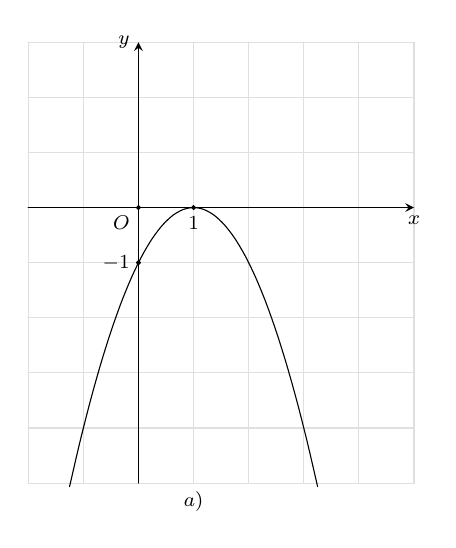
\begin{tikzpicture}[scale=.7, font=\footnotesize, line join=round, line cap=round, >=stealth]
		\draw[gray!50,opacity=.5](-2,-5)grid(5,3);
		\draw[->](-2,0)--(0,0)node[below left]{$O$}--(5,0)node[below]{$x$};
		\draw[->](0,-5)--(0,3)node[left]{$y$};
		\draw[smooth,domain=-1.25:3.25]plot(\x,{-(\x)^2+2*(\x)-1});
		\draw (1,-5)node[below]{$a)$};
		\draw(1,0)node[below]{$1$};
		\draw(0,-1)node[left]{$-1$};
		\foreach \x in{0,1}\draw[fill](\x,0)circle(1pt);
		\draw[fill](0,-1)circle(1pt);
	\end{tikzpicture}\hspace*{1cm}
	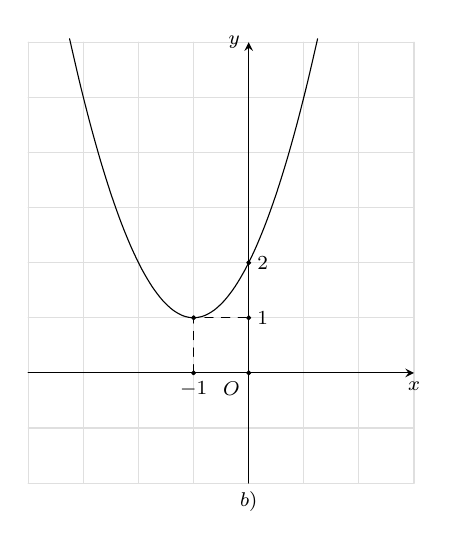
\begin{tikzpicture}[scale=.7, font=\footnotesize, line join=round, line cap=round, >=stealth]
		\draw[gray!50,opacity=.5](-4,-2)grid(3,6);
		\draw[->](-4,0)--(0,0)node[below left]{$O$}--(3,0)node[below]{$x$};
		\draw[->](0,-2)--(0,6)node[left]{$y$};
		\draw[smooth,domain=-3.25:1.25]plot(\x,{(\x)^2+2*(\x)+2});
		\draw (0,-2)node[below]{$b)$};
		\draw(0,1)node[right]{$1$};
		\draw(0,2)node[right]{$2$};
		\draw(-1,0)node[below]{$-1$};
		\draw[dashed](-1,0)--(-1,1)--(0,1);
		\foreach \x in {0,1,2}\draw[fill](0,\x)circle(1pt);
		\draw[fill](-1,0)circle(1pt);
		\draw[fill](-1,1)circle(1pt);
	\end{tikzpicture}\hspace*{1cm}
	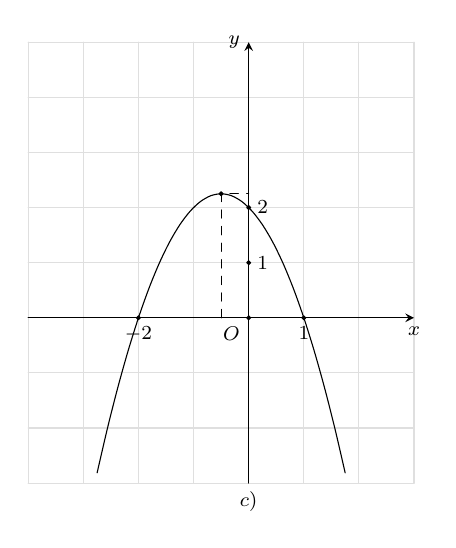
\begin{tikzpicture}[scale=.7, font=\footnotesize, line join=round, line cap=round, >=stealth]
		\draw[gray!50,opacity=.5](-4,-3)grid(3,5);
		\draw[->](-4,0)--(0,0)node[below left]{$O$}--(3,0)node[below]{$x$};
		\draw[->](0,-3)--(0,5)node[left]{$y$};
		\draw[smooth,domain=-2.75:1.75]plot(\x,{-(\x)^2-(\x)+2});
		\draw (0,-3)node[below]{$c)$};
		\draw(0,1)node[right]{$1$};
		\draw(0,2)node[right]{$2$};
		\draw(-2,0)node[below]{$-2$};
		\draw(1,0)node[below]{$1$};
		\draw[dashed](-0.5,0)--(-1/2,2.25)--(0,2.25);
		\foreach \x in {-2,0,1}\draw[fill](\x,0)circle(1pt);
		\foreach \x in {1,2}\draw[fill](0,\x)circle(1pt);
		\draw[fill](-1/2,2.25)circle(1pt);
	\end{tikzpicture}
	\loigiai{
		\begin{enumEX}[a)]{1}
			\item \immini{Từ đồ thị hình a) ta có nghiệm của tam thức bậc hai $f(x)$ là $x=1$. Bảng xét dấu của tam thức là}{
				
\begin{tikzpicture}
					\tkzTabInit[deltacl=0.6,espcl=2.5,lgt=2,nocadre=false]
					{$x$/0.6,$f(x)$/0.6}
					{$-\infty$,$1$,$+\infty$}
					\tkzTabLine{,-,0,-,}
				\end{tikzpicture}
			}
			\item \immini{Từ đồ thị hình b) ta có tam thức bậc hai $f(x)$ vô nghiệm. Bảng xét dấu của tam thức là}{
				
\begin{tikzpicture}
					\tkzTabInit[deltacl=0.6,espcl=2.5,lgt=2,nocadre=false]
					{$x$/0.6,$f(x)$/0.6}
					{$-\infty$,,$+\infty$}
					\tkzTabLine{,,+,}
				\end{tikzpicture}
			}
			\item \immini{Từ đồ thị hình c) ta có nghiệm của tam thức bậc hai $f(x)$ là $x_1=-2$ và $x_2=1$. Bảng xét dấu của tam thức là}{
				
\begin{tikzpicture}
					\tkzTabInit[deltacl=0.6,espcl=2.5,lgt=2,nocadre=false]
					{$x$/0.6,$f(x)$/0.6}
					{$-\infty$,$-2$,$1$,$+\infty$}
					\tkzTabLine{,-,0,+,0,-,}
				\end{tikzpicture}
			}
		\end{enumEX}
	}
\end{bt}

% từ: cau-hoi/lop10/0D7_Bat_phuong_trinh_bac_2_mot_an/0D7-1-3_Bai_toan_xet_dau_biet_BXD_do_thi.tex
\begin{bt}%[0D7H1-3]%[Tex hóa SGK CD-CT,T7/22, Nguyễn Vương Hiển]%[ma:d8e1b472]
	Tìm nghiệm và lập bảng xét dấu của tam thức bậc hai $f(x)$ với đồ thị được cho ở mỗi hình\\
	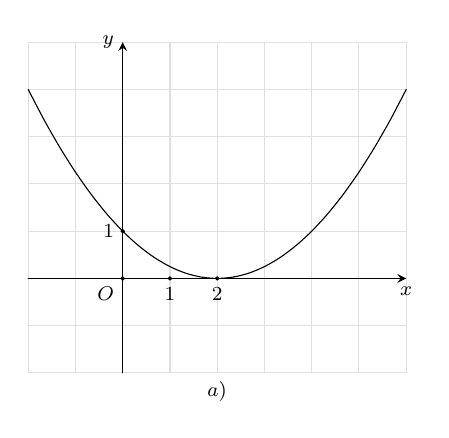
\begin{tikzpicture}[scale=.6, font=\footnotesize, line join=round, line cap=round, >=stealth]
		\draw[gray!50,opacity=.5](-2,-2)grid(6,5);
		\draw[->](-2,0)--(0,0)node[below left]{$O$}--(6,0)node[below]{$x$};
		\draw[->](0,-2)--(0,5)node[left]{$y$};
		\draw[smooth,domain=-2:6]plot(\x,{1/4*(\x)^2-(\x)+1});
		\draw (2,-2)node[below]{$a)$};
		\draw(1,0)node[below]{$1$};
		\draw(2,0)node[below]{$2$};
		\draw(0,1)node[left]{$1$};
		\foreach \x in{0,1,2}\draw[fill](\x,0)circle(1pt);
		\draw[fill](0,1)circle(1pt);
	\end{tikzpicture}\hspace*{1cm}
	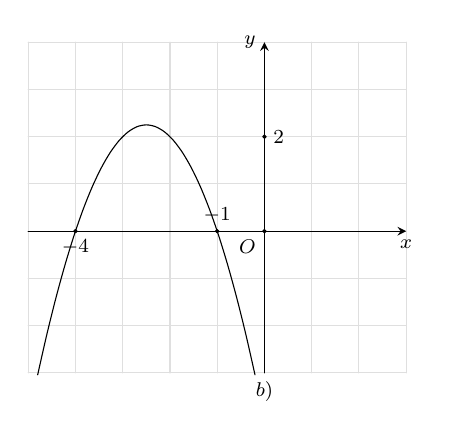
\begin{tikzpicture}[scale=.6, font=\footnotesize, line join=round, line cap=round, >=stealth]
		\draw[gray!50,opacity=.5](-5,-3)grid(3,4);
		\draw[->](-5,0)--(0,0)node[below left]{$O$}--(3,0)node[below]{$x$};
		\draw[->](0,-3)--(0,4)node[left]{$y$};
		\draw[smooth,domain=-4.8:-0.2]plot(\x,{-(\x)^2-5*(\x)-4});
		\draw (0,-3)node[below]{$b)$};
		\draw(-4,0)node[below]{$-4$};
		\draw(0,2)node[right]{$2$};
		\draw(-1,0)node[above]{$-1$};
		\foreach \x in{-4,-1,0}\draw[fill](\x,0)circle(1pt);
		\draw[fill](0,2)circle(1pt);
	\end{tikzpicture}\hspace*{1cm}
	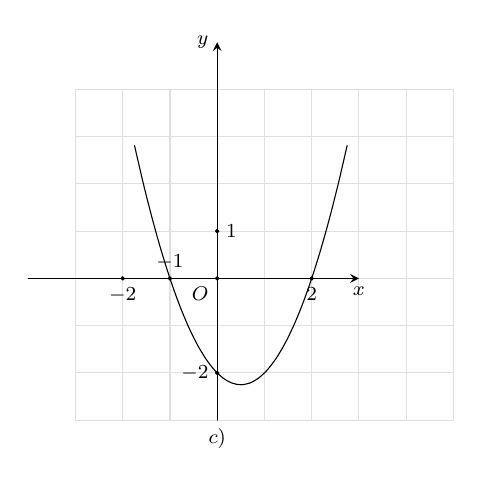
\begin{tikzpicture}[scale=.6, font=\footnotesize, line join=round, line cap=round, >=stealth]
		\draw[gray!50,opacity=.5](-3,-3)grid(5,4);
		\draw[->](-4,0)--(0,0)node[below left]{$O$}--(3,0)node[below]{$x$};
		\draw[->](0,-3)--(0,5)node[left]{$y$};
		\draw[smooth,domain=-1.75:2.75]plot(\x,{(\x)^2-(\x)-2});
		\draw (0,-3)node[below]{$c)$};
		\draw(0,1)node[right]{$1$};
		\draw(0,-2)node[left]{$-2$};
		\draw(-2,0)node[below]{$-2$};
		\draw(-1,0)node[above]{$-1$};
		\draw(2,0)node[below]{$2$};
		\foreach \x in {-2,-1,0,2}\draw[fill](\x,0)circle(1pt);
		\foreach \x in {-2,1}\draw[fill](0,\x)circle(1pt);
	\end{tikzpicture}
	\loigiai{
		\begin{enumEX}[a)]{1}
			\item \immini{Từ đồ thị hình a) ta có nghiệm của tam thức bậc hai $f(x)$ là $x=2$. Bảng xét dấu của tam thức là}{
				
\begin{tikzpicture}
					\tkzTabInit[deltacl=0.6,espcl=2.5,lgt=2,nocadre=false]
					{$x$/0.6,$f(x)$/0.6}
					{$-\infty$,$2$,$+\infty$}
					\tkzTabLine{,+,0,+,}
				\end{tikzpicture}
			}
			\item \immini{Từ đồ thị hình b) ta có tam thức bậc hai $f(x)$ có $2$ nghiệm $x_1=-4$ và $x_2=-1$. Bảng xét dấu của tam thức là}{
				
\begin{tikzpicture}
					\tkzTabInit[deltacl=0.6,espcl=2.5,lgt=2,nocadre=false]
					{$x$/0.6,$f(x)$/0.6}
					{$-\infty$,$-4$,$-1$,$+\infty$}
					\tkzTabLine{,-,0,+,0,-,}
				\end{tikzpicture}
			}
			\item \immini{Từ đồ thị hình c) ta có nghiệm của tam thức bậc hai $f(x)$ là $x_1=-1$ và $x_2=2$. Bảng xét dấu của tam thức là}{
				
\begin{tikzpicture}
					\tkzTabInit[deltacl=0.6,espcl=2.5,lgt=2,nocadre=false]
					{$x$/0.6,$f(x)$/0.6}
					{$-\infty$,$-1$,$2$,$+\infty$}
					\tkzTabLine{,+,0,-,0,+,}
				\end{tikzpicture}
			}
		\end{enumEX}
	}
\end{bt}

% từ: cau-hoi/lop10/0D7_Bat_phuong_trinh_bac_2_mot_an/0D7-1-3_Bai_toan_xet_dau_biet_BXD_do_thi.tex
\begin{bt}%[0D7H1-3]%[Tex hóa SGK CD-CT,T7/22, Bùi Mạnh Tiến]%[ma:99795839]
	Dựa vào đồ thị của các hàm số bậc hai được cho trong hình dưới đây
	\begin{enumEX}{2}
		\item \immini
		{
			$f(x)=2x^2+5x+2$;
		}
		{
			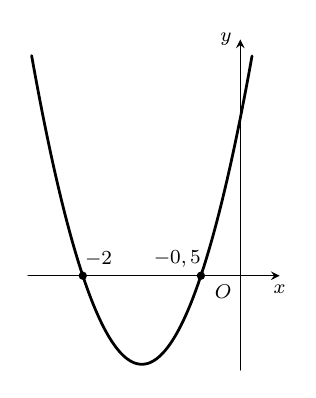
\begin{tikzpicture}[line join = round, line cap = round,>=stealth,font=\footnotesize,scale=1]
				\def\xmin{-2.7}
				\def\xmax{0.5}
				\def\ymin{-1.2}
				\def\ymax{3}
				\clip (\xmin,\ymin) rectangle (\xmax+0.1,\ymax+0.15);
				\draw[->] (\xmin,0) -- (\xmax,0) node[below] {$x$};
				\draw[->] (0,\ymin) -- (0,0) node[below left] {$O$} -- (0,\ymax) node[left] {$y$};
				\draw[smooth, line width=1,samples=100] plot[domain=-2.65:0.15] (\x,{2*(\x)^2+5*(\x)+2});
				\fill (-2,0) circle (1.5pt);
				\fill (-0.5,0) circle (1.5pt);
				\draw (-1.8,0) node[above] {$-2$};
				\draw (-0.8,0) node[above] {$-0,5$};
			\end{tikzpicture}
		}
		\item \immini
		{
			$g(x)=-x^2+3x-3$;
		}
		{
			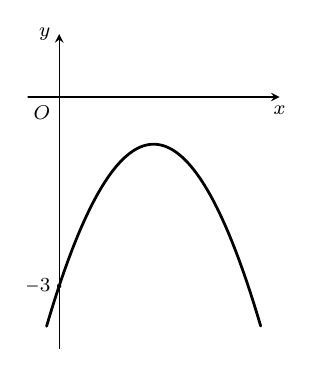
\begin{tikzpicture}[line join = round, line cap = round,>=stealth,font=\footnotesize,scale=0.8]
				\def\xmin{-0.5}
				\def\xmax{3.5}
				\def\ymin{-4}
				\def\ymax{1}
				\clip (\xmin,\ymin) rectangle (\xmax+0.1,\ymax+0.1);
				\draw[->] (\xmin,0) -- (\xmax,0) node[below] {$x$};
				\draw[->] (0,\ymin) -- (0,0) node[below left] {$O$} -- (0,\ymax) node[left] {$y$};
				\draw[smooth, line width=1,samples=100] plot[domain=-0.2:3.2] (\x,{-(\x)^2+3*(\x)-3});
				\fill (0,-3) circle (1pt) node[left] {$-3$};
			\end{tikzpicture}
		}
		\item \immini
		{
			$h(x)=-x^2+4x-4$;
		}
		{
			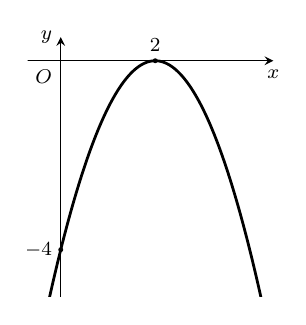
\begin{tikzpicture}[line join = round, line cap = round,>=stealth,font=\footnotesize,scale=0.6]
				\def\xmin{-0.7}
				\def\xmax{4.5}
				\def\ymin{-5}
				\def\ymax{0.5}
				\clip (\xmin,\ymin) rectangle (\xmax+0.1,\ymax+0.2);
				\draw[->] (\xmin,0) -- (\xmax,0) node[below] {$x$};
				\draw[->] (0,\ymin) -- (0,0) node[below left] {$O$} -- (0,\ymax) node[left] {$y$};
				\draw[smooth, line width=1,samples=100] plot[domain=-.25:4.25] (\x,{-(\x)^2+4*(\x)-4});
				\fill (2,0) circle (1.5pt);
				\fill (0,-4) circle (1.5pt);
				\draw (2,0) node[above] {$2$};
				\draw (0,-4) node[left] {$-4$};
			\end{tikzpicture}
		}
	\end{enumEX}
	Xét dấu của tam thức bậc hai tương ứng
	\loigiai{
		\begin{enumerate}
			\item $f(x)>0$ trên khoảng $(-\infty;-2)$ và $(-0{,}5;+\infty)$.\\
			$f(x)<0$ trên khoảng $(-2;-0{,}5)$.
			\item $g(x)<0$ với mọi $x \in \mathbb{R}$.
			\item $h(x)<0$ với mọi $x \ne 2$.
		\end{enumerate}
	}
\end{bt}

% từ: cau-hoi/lop10/0D7_Bat_phuong_trinh_bac_2_mot_an/0D7-1-3_Bai_toan_xet_dau_biet_BXD_do_thi.tex
\begin{bt}%[0D7H1-3]%[Tex hóa SGK CD-CT,T7/22, Bùi Mạnh Tiến]%[ma:5d2176e5]
	Dựa vào đồ thị của các hàm số bậc hai được cho trong hình dưới đây, xét dấu của tam thức bậc hai tương ứng:
	\begin{enumEX}{2}
		\item 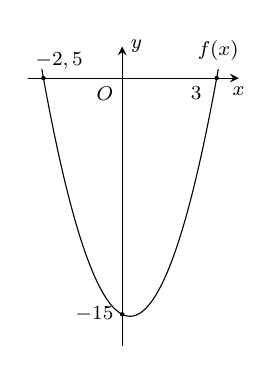
\begin{tikzpicture}[line join = round, line cap = round,>=stealth,font=\footnotesize,scale=0.4]
			\def\xmin{-3}
			\def\xmax{3.7}
			\def\ymin{-8.5}
			\def\ymax{1}
			\clip (\xmin,\ymin) rectangle (\xmax+0.4,\ymax+0.6);
			\draw[->] (\xmin,0) -- (\xmax,0) node[below] {$x$};
			\draw[->] (0,\ymin) -- (0,0) node[below left] {$O$} -- (0,\ymax) node[right] {$y$};
			\draw[smooth,samples=100] plot[domain=-2.55:3.05] (\x,{(\x-3)*(\x+2.5)}) node[above] {$f(x)$};
			\fill (-2.5,0) circle (2pt);
			\draw (-2,0) node[above] {$-2,5$};
			\fill (3,0) circle (2pt);
			\draw (2.8,0) node[below left] {$3$};
			\fill (0,-7.5) circle (2pt);
			\draw (0,-7.5) node[left] {$-15$};
		\end{tikzpicture}
		\item 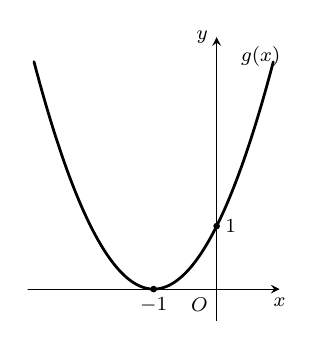
\begin{tikzpicture}[line join = round, line cap = round,>=stealth,font=\footnotesize,scale=0.8]
			\def\xmin{-3}
			\def\xmax{1}
			\def\ymin{-0.5}
			\def\ymax{4}
			\clip (\xmin,\ymin) rectangle (\xmax+0.1,\ymax+0.15);
			\draw[->] (\xmin,0) -- (\xmax,0) node[below] {$x$};
			\draw[->] (0,\ymin) -- (0,0) node[below left] {$O$} -- (0,\ymax) node[left] {$y$};
			\draw[smooth, line width=1,samples=100] plot[domain=-2.9:0.9] (\x,{(\x+1)^2});
			\draw (0.7,3.4) node[above] {$g(x)$}; 
			\fill (-1,0) circle (1.5pt) node[below] {$-1$};
			\fill (0,1) circle (1.5pt) node[right] {$1$};
		\end{tikzpicture}
		\item 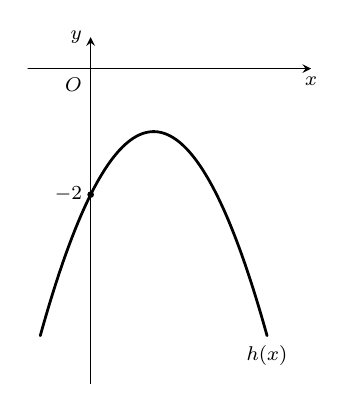
\begin{tikzpicture}[line join = round, line cap = round,>=stealth,font=\footnotesize,scale=0.8]
			\def\xmin{-1}
			\def\xmax{3.5}
			\def\ymin{-5}
			\def\ymax{0.5}
			\clip (\xmin,\ymin) rectangle (\xmax+0.1,\ymax+0.15);
			\draw[->] (\xmin,0) -- (\xmax,0) node[below] {$x$};
			\draw[->] (0,\ymin) -- (0,0) node[below left] {$O$} -- (0,\ymax) node[left] {$y$};
			\draw[smooth, line width=1,samples=100] plot[domain=-0.8:2.8] (\x,{-(\x-1)^2-1}) node[below] {$h(x)$};
			\fill (0,-2) circle (1.5pt) node[left] {$-2$};
		\end{tikzpicture}
	\end{enumEX}
	\loigiai{
		\begin{enumerate}
			\item $f(x)$ dương trên $(-\infty;-2{,}5)$ và $(3;+\infty)$, âm trên $(-2{,}5;3)$.
			\item $g(x)$ dương với mọi $x \ne -1$.
			\item $h(x)$ âm với mọi $x \in \mathbb{R}$.
		\end{enumerate}
	}
\end{bt}

% từ: cau-hoi/lop10/0D7_Bat_phuong_trinh_bac_2_mot_an/0D7-2-2_Giai_bat_phuong_trinh_bac_hai_biet_BXD_do_thi.tex
\begin{bt}%[0D7H2-2]%[Dự án đề kiểm tra HKII NH22-23-BCTuan]%[THPT Thực Hành Sài Gòn]%[ma:13f25e9d]
\immini
{
	\begin{enumerate}
		\item 	Dựa vào đồ thị của hàm số bậc hai $y=f(x)$ như hình bên. Hãy tìm tập nghiệm của bất phương trình $f(x) \ge 0$.
		\item Cho bất phương trình $2x^2+2(m-3) x+3(m^2-3) \ge 0$ ($m$ là tham số thực). Tìm tham số $m$ để tập nghiệm của bất phương trình là $\mathbb{R}$.
	\end{enumerate}
	
}
{
\begin{tikzpicture}[line join=round, line cap=round,>=stealth,font=\footnotesize]
	\tikzset{every node/.style={scale=0.9}}
	\draw[->] (-3.1,0)--(3.1,0) node[below left] {$x$};
	\draw[->] (0,-1)--(0,4.1) node[below left] {$y$};
	\draw (0,0) node [below left] {$O$};
	\foreach \x in {-2}
	\draw[thin] (\x,1pt)--(\x,-1pt) node [above left=-3pt] {$\x$};
	\foreach \y in {3}
	\draw[thin] (1pt,\y)--(-1pt,\y) node [above left] {$\y$};
	\draw (1.5,0) node[below left=-2pt]{$\tfrac{3}{2}$};
	\begin{scope}
		\clip (-3,-2) rectangle (3,4);
		\draw[samples=200,domain=-2.25:1.75,smooth,variable=\x] plot (\x,{-1*(\x)^2-0.5*(\x)+3});
	\end{scope}
\end{tikzpicture}
}
\loigiai{
\begin{enumerate}
	\item Dựa vào đồ thị hàm số ta có $f(x)\ge 0\Leftrightarrow -2\le x\le \dfrac{3}{2}$.\\
	Vậy tập nghiệm của bất phương trình là $S=\left[-2;\dfrac{3}{2}\right]$.
	\item Để tập nghiệm của bất phương trình $2x^2+2(m-3) x+3(m^2-3) \ge 0$ là $\mathbb{R}$ thì
	$$\heva{& a>0 \\ & \Delta'\le 0}\Leftrightarrow \heva{& 2>0 \\ & (m-3)^2-6(m^2-3)\le 0}\Leftrightarrow -5m^2-6m+27\le 0\Leftrightarrow \hoac{& m\le -3 \\ & m\ge \dfrac{9}{5}.}$$
\end{enumerate}
}
\end{bt}

% từ: cau-hoi/lop10/0D7_Bat_phuong_trinh_bac_2_mot_an/0D7-2-6_Bai_toan_co_tham_so.tex
\begin{bt}%[0D7H2-6]%[ma:8b30459e]
	Có bao nhiêu  giá trị nguyên của tham số $m$ thuộc đoạn $\left[-10;5\right]$ để phương trình $x^2-(m+1)x+3m-5=0$ có hai nghiệm phân biệt?
	 \shortans{13}
	 \loigiai{
		Ta  có $\Delta=[-(m+1)]^2-4\cdot 1\cdot (3m-5)=m^2-10m+21$.\\
		Để phương trình $x^2-(m+1)x+3m-5=0$ có hai nghiệm phân  biệt thì \[\Delta > 0\text{ hay } m^2-10m+21> 0.\]
		Tam thức bậc hai $m^2-10m+21$ có  $a=1> 0$ và có hai nghiệm $m_1=3,m_2=7$.\\
		Do đó, $m^2-10m+21> 0$ khi $m\in (-\infty;3)\cup (7;+\infty)$.\\ 
		Mà $m\in  \mathbb{Z}$ và $m\in \left[-10;5\right]$ nên có $13$ giá trị nguyên của tham số $m$ thỏa mãn.
	} 
\end{bt}

% từ: cau-hoi/lop10/0D7_Bat_phuong_trinh_bac_2_mot_an/0D7-2-6_Bai_toan_co_tham_so.tex
\begin{bt}%[0D7V2-6]%[ma:4272f6be]
	Có bao nhiêu giá trị nguyên của tham số $m$ thuộc  khoảng $\left(-50;50\right)$ để phương trình $x^2+(m-2)x-8m+1=0$ có hai nghiệm phân biệt?
	 \loigiai{
		Ta có  $a=1\ne 0,b=m-2,c=-8m+1$.\\
		Phương trình có hai nghiệm phân biệt khi và chỉ khi \[\Delta=(m-2)^2-4(-8m+1) > 0\Leftrightarrow m^2+28m > 0.\] 
		Xét  $m^2+28m=0\Leftrightarrow m=0$ hoặc $m=-28$.\\
		Bảng xét dấu 
		\begin{center}
			
\begin{tikzpicture}[>=stealth]
					 \tkzTabInit[nocadre=false,lgt=1.5,espcl=2,deltacl=0.6]{$x$/.7,$f (x)$/.7}
						{$-\infty$,$0$,$28$,$+\infty$} 
					 \tkzTabLine{,+,$0$,-,$0$,+,}
				\end{tikzpicture}
		\end{center}
		Ta có $m^2+28m > 0\Leftrightarrow m\in (-\infty;-28)\cup (0;+\infty)$.\\ 
		Mà $m$ nguyên  thuộc khoảng $\left(-50;50\right)$ nên $m\in\{-49;-48;\ldots;-29\}\cup\{1;2;3;\ldots;49\}$.
		Vậy có $70$ giá trị nguyên của tham  số $m$ thỏa mãn yêu cầu bài toán.
	} 
\end{bt}

% từ: cau-hoi/lop10/0D7_Bat_phuong_trinh_bac_2_mot_an/0D7-2-6_Bai_toan_co_tham_so.tex
\begin{bt}%[0D7H2-6]%[ma:b3d22982]
	Tìm tất cả các giá trị thực của tham số $m$ để phương trình sau có hai nghiệm phân biệt
	\[
	-x^2 + (m + 2)x - 4 = 0.
	\]
	\loigiai{
		Ta có $\Delta = (m + 2)^2 - 16 = m^2 + 4m - 12$.\\
		Để phương trình đã cho có hai nghiệm phân biệt thì $\Delta > 0 \Rightarrow m^2 + 4m - 12 > 0$.\\
		Đặt $f(m)=m^2 + 4m - 12$. Ta có bảng xét dấu
		\begin{center}
			
\begin{tikzpicture}[>=stealth,line join=round,line cap=round,font=\footnotesize,scale=1]
				\tkzTabInit[nocadre=false,lgt=1.2,espcl=3,deltacl=.55]
				{$x$/0.7, $f(m)$/0.7}
				{$-\infty$,$-6$,$2$,$+\infty$}
				\tkzTabLine{,+,$0$,-,$0$,+,}
			\end{tikzpicture}
		\end{center}
		Vậy với $m \in (-\infty, -6) \cup (2, +\infty)$ thì phương trình đã cho có hai nghiệm phân biệt.
	}
\end{bt}

% từ: cau-hoi/lop10/0D7_Bat_phuong_trinh_bac_2_mot_an/0D7-2-6_Bai_toan_co_tham_so.tex
\begin{bt}%[0D7H2-6]%[ma:e29184f4]
	Tìm tất cả giá trị $m$ để phương trình sau có hai nghiệm phân biệt: $x^2+(m-2) x-8 m+1=0$.
	\loigiai{
	Ta có $a=1 \neq 0$, $b=m-2$, $c=-8 m+1$.\\
	Phương trình có hai nghiệm phân biệt khi và chỉ khi
	$$\Delta=(m-2)^2-4(-8 m+1)>0 \Leftrightarrow m^2+28 m>0.$$
	Xét $m^2+28 m=0 \Leftrightarrow \hoac{&m=0 \\& m=-28.}$\\
	Bảng xét dấu:
		\begin{center}
			
\begin{tikzpicture}
				\tkzTabInit[nocadre=false,lgt=3,espcl=2,deltacl=0.6]
				{$x$ /0.6,$m^2+28m$ /0.6}
				{$-\infty$,$-28$,$0$,$+\infty$}
				\tkzTabLine{,+,$0$,-,$0$,+,}
			\end{tikzpicture}
		\end{center}
		Ta có $m^2+28 m>0 \Leftrightarrow m \in(-\infty;-28) \cup(0;+\infty)$.\\
		Vậy với $m \in(-\infty;-28) \cup(0;+\infty)$ thì phương trình đã cho có hai nghiệm phân biệt.
		}
	\end{bt}

% từ: cau-hoi/lop10/0D7_Bat_phuong_trinh_bac_2_mot_an/0D7-2-7_Toan_thuc_te_ung_dung_bat_phuong_trinh_bac_2.tex
\begin{bt}%[0D7V2-7]%[Dự án đề kiểm tra GKII NH22-23- Hiếu Phan]%[THPT Trần Khai Nguyên]%[ma:42e49897]
   Một mảnh vườn hình chữ nhật có chu vi $ 42 $ cm. Biết diện tích của mảnh vườn ít nhất là $ 108~\mathrm{cm^2} $. Hỏi chiều dài của mảnh vườn nằm trong khoảng nào?
    \loigiai{
    Gọi chiều dài của mảnh vườn hình chữ nhật là $ x (x>0)$ cm  .\\
    Khi đó chiều rộng của mảnh vườn là $ 21-x $ cm.\\
    Diện tích của mảnh vườn ít nhất là $ 108~\mathrm{cm^2} $ nên suy ra
    $$ x(21-x)\le 108 \Leftrightarrow -x^2+21x-108\le  0\Leftrightarrow 9\le x \le 12.$$
    Vậy chiều dài của mảnh vườn nằm trong khoảng từ $ 9 $ cm đến $ 12 $ cm.
}
\end{bt}

% từ: cau-hoi/lop10/0D7_Bat_phuong_trinh_bac_2_mot_an/0D7-3-1_Phuong_trinh_can.tex
\begin{ex}%[0D7N3-1]%[ma:3f9fa9f7]
	Cho phương trình $\sqrt{4x+3}=\sqrt{5x-8}$. 
	\choiceTF 
		 {\True Phương trình có một nghiệm}
		 {\True Phương trình có nghiệm là $x=11$}
		{Phương trình vô  nghiệm}
		{Phương trình có  hai nghiệm phân biệt}
	\loigiai{ 
		Bình phương hai vế của phương trình $\sqrt{4x+3}=\sqrt{5x-8}$ ta  được
		\[4x+3=5x-8\Leftrightarrow x=11\] 
		 Thay giá trị $x=11$ vào phương trình ta thấy thỏa mãn.\\
		Vậy phương trình có  một nghiệm là $x=11$.
	} 
\end{ex}

% từ: cau-hoi/lop10/0D7_Bat_phuong_trinh_bac_2_mot_an/0D7-3-2_Phuong_trinh_can.tex
\begin{ex}%[0D7H3-2]%[ma:3d3b3ff0]
	Cho  phương trình $\sqrt{2x^2-5x+11}=x+1$.
	 \choiceTF
		 {\True Phương trình có hai nghiệm phân biệt}
		{Phương trình có một  nghiệm}
		{\True $x=2$ là nghiệm của phương  trình}
		{\True $x=5$ là nghiệm  của phương trình}
	\loigiai{ 
		Bình phương hai vế  của phương trình $\sqrt{2x^2-5x+11}=x+1$ ta được
		\begin{eqnarray*}
			 && 2x^2-5x+11=(x+1)^2\\
			&\Leftrightarrow& 2x^2-5x+11=x^2+2x+1\\ 
			 &\Leftrightarrow& x^2-7x+10=0\\
			&\Leftrightarrow&  \hoac{&x=2\\&x=5.}
		\end{eqnarray*}
		Thay lần lượt các giá trị  trên của $x$ vào phương trình ta thấy cả hai đều thỏa mãn.\\
		Vậy phương trình có nghiệm  là $x=2$, $x=5$.
	 }
\end{ex}

% từ: cau-hoi/lop10/0D7_Bat_phuong_trinh_bac_2_mot_an/0D7-3-3_Phuong_trinh_can_thuc_co_tham_so.tex
\begin{bt}%[0D7C3-3]%[ma:e9c38390]
		Tìm điều kiện của tham số $m$ để phương trình sau có hai nghiệm phân biệt:
		$$
		\sqrt{-x^2+6x+m}=x-1. \quad \hfill (1)
		$$
		 
		\loigiai{
			Trước hết ta giải bất phương trình $x-1\geq 0\Leftrightarrow x\geq 1.\qquad (*)$\\ 
			Bình phương hai vế của phương trình $(1)$ ta được $$-x^2+6x+m=(x-1)^2\Leftrightarrow m=2x^2-8x+1.\qquad (2)$$ 
			Phương trình $(1)$ có hai nghiệm phân biệt khi và chỉ khi phương trình $(2)$ có hai nghiệm phân biệt thỏa mãn $(*)$.
		}
	\end{bt}

% từ: cau-hoi/lop10/0D7_Bat_phuong_trinh_bac_2_mot_an/0D7-3-5_Phuong_trinh_khac_quy_ve_phuong_trinh_bac_2.tex
\begin{bt}%[0D7H3-5]%[ma:19ec6f93]
	Giải các phương trình sau:
	\begin{enumEX}{2}
		\item $\dfrac{2x+1}{3x+2}=\dfrac{x+1}{x-2}$.
		\item $1+\dfrac{2}{x-2}=\dfrac{10}{x+3}-\dfrac{50}{(2-x)(x+3)}$.
		\item $\dfrac{4}{2x+1}+\dfrac{3}{2x+2}=\dfrac{2}{2x+3}+\dfrac{1}{2x+4}$.
		\item $1+\dfrac{4}{2-x^{2}}=\dfrac{5}{x^{2}}$.
	\end{enumEX}
	\loigiai{
		\begin{enumEX}{1}
			\item Điều kiện xác định $\heva{&x \ne \dfrac{2}{3}\\& x \ne 2.}$\\
			Phương trình tương đương với
				\begin{eqnarray*}
				& & (2x+1)(x-2)=(x+1)(3x+2) \\
				& \Leftrightarrow &  2x^{2}-4x+x-2=3x^{2}+2x+3x+2 \\
				& \Leftrightarrow & x^{2}+8x+4=0\\
				& \Leftrightarrow &x = -4 \pm 2\sqrt{3}
			\end{eqnarray*}
			Vậy phương trình có nghiệm $x = -4 \pm 2\sqrt{3}$.
			\item Điều kiện xác định $\heva{&x \ne -3\\& x \ne 2.}$\\
				Phương trình tương đương với $(2-x)(x+3)-2(x+3)=10(2-x)-50 \Leftrightarrow x^{2}-7x-30=0 \Leftrightarrow \hoac{&x=10\\&x=-3.}$\\
				Đối chiếu với điều kiện, vậy phương trình có nghiệm $x=10$.
			\item Điều kiện xác định $x \ne \{-2;-\dfrac{2}{3};-1;-\dfrac{1}{2}\}$.\\
			Phương trình tương đương với 
				\begin{eqnarray*}
				& & \dfrac{4}{2x+1}-\dfrac{2}{2x+3}=\dfrac{1}{2x+4}-\dfrac{3}{2x+2} \\
				& \Leftrightarrow &  \dfrac{4}{2x+1}-\dfrac{2}{2x+3}=\dfrac{1}{2x+4}-\dfrac{3}{2x+2} \\
				& \Leftrightarrow & (4x+10) \left( \dfrac{1}{4x^{2}+8x+3}+\dfrac{1}{4x^{2}+12x+8}\right)\\
				& \Leftrightarrow & (4x+10)(4x^{2}+8x+3+4x^{2}+12x+8)=0\\
				& \Leftrightarrow &  (4x+10)(8x^{2}+20x+11)=0 \\
				& \Leftrightarrow & \hoac{&4x+10=0\\&8x^{2}+20x+11=0} \\
				& \Leftrightarrow &\hoac{&x=-\dfrac{5}{2}\\&x=\dfrac{-5 \pm \sqrt{3}}{4}.}
			\end{eqnarray*}
			Đối chiếu với điều kiện, vậy phương trình có nghiệm $\hoac{&x=-\dfrac{5}{2}\\&x=\dfrac{-5 \pm \sqrt{3}}{4}.}$
			\item Điều kiện xác định $\heva{&x \ne 0\\& x \ne 2.}$\\
			Phương trình tương đương với\\ $x^{2}+\dfrac{4x^{2}}{(2-x)^{2}}=5 \Leftrightarrow x^{2}- \dfrac{4x^{2}}{2-x} +\dfrac{4x^{2}}{(2-x)^{2}} + \dfrac{4x^{2}}{2-x}-5=0 \Leftrightarrow \left( x-\dfrac{2x}{2-x}\right)^{2} + \dfrac{4x^{2}}{2-x}-5=0 \\ \Leftrightarrow \left(\dfrac{x^{2}}{2-x} \right)^{2} + \dfrac{4x^{2}}{2-x}-5=0$.\\
			Đặt $t=\dfrac{x^{2}}{2-x}$, phương trình trở thành $t^{2}+4t-5=0 \Leftrightarrow \hoac{&t=1\\&t=-5.}$\\
			Với $t=1$ ta có $\dfrac{x^{2}}{2-x} =1 \Leftrightarrow x^{2}+x-2=0 \Leftrightarrow \hoac{&x=1\\&x=-2.}$ (Thỏa mãn)\\
			Với $t=-5$ ta có $\dfrac{x^{2}}{2-x} =-5	 \Leftrightarrow x^{2}-5x+10=0$ (Vô nghiệm).
				
		Vậy phương trình có nghiệm $x=1$ và $x=-2$.
		\end{enumEX}
	}		
\end{bt}

% từ: cau-hoi/lop10/0D7_Bat_phuong_trinh_bac_2_mot_an/0D7-3-6_Toan_hinh_toan_thuc_te_ung_dung_phuong_trinh.tex
\begin{bt}%[0D7C3-6]%[ma:a9a80641]
	Cho lục giác $ABCDEF$ có $AB \perp EF$; $BC \perp DE$; $AF \parallel CD$; $AF=CD$; $AB=4$; $BE=26$; $EF=16$; $AF=10$. Gọi $H$ là  giao điểm của $AB$ và $EF$; $K$ là giao điểm của $BC$ và $ED$, khi đó tứ giác $HBKE$ là hình chữ nhật, đặt $x=AH$; $x>0$. Hãy tính độ dài $x$.
	\begin{center}
		\begin{tikzpicture}[line cap=round,line join=round,font=\footnotesize,>=stealth,scale=0.3]
				 \path
					(0,0) coordinate (B) 
					 ($(B)+(90:4)$) coordinate (A)
					 ($(A)+(90:6)$) coordinate (H)
					($(H)+(0:8)$) coordinate  (F)
					($(F)+(0:16)$) coordinate  (E)
					($(B)+(0:16)$)  coordinate (C)
					($(C)+(0:8)$) coordinate (K) 
					($(K)+(90:6)$) coordinate  (D);
				\draw (B)--(A)--(H)  node [midway,left] {$x$}--(E)--(K)--cycle (A)--(F)
					 (C)--(D);
				\foreach \x/\g in {A/-180,B/-135,C/-90,K/-45,D/0,E/45,F/90,H/135}{ 
					\fill (\x)  circle (4pt) node[shift=(\g:3mm)] {$\x$};}
			\end{tikzpicture}
	\end{center}
	\shortans{6} 
	 \loigiai{
		\begin{center}
			\begin{tikzpicture}[line cap=round,line join=round,font=\footnotesize,>=stealth,scale=0.3]
					 \path
						(0,0) coordinate (B) 
						($(B)+(90:4)$) coordinate (A) 
						($(A)+(90:6)$)  coordinate (H)
						($(H)+(0:8)$)  coordinate (F)
						($(F)+(0:16)$) coordinate (E) 
						($(B)+(0:16)$)  coordinate (C)
						 ($(C)+(0:8)$) coordinate (K)
						($(K)+(90:6)$) coordinate  (D);
					\draw (B)--(A) node [midway,left] {$4$}--(H) node [midway,left]  {$x$}--(F)--(E) node [midway,above] {$16$}--(K)--cycle (A)--(F) node[midway,above left] {$10$}
						 (C)--(D)
						(B)--(E)  node[midway,above left] {$26$};
					 \foreach \x/\g in {A/-180,B/-135,C/-90,K/-45,D/0,E/45,F/90,H/135}{
						 \fill (\x) circle (4pt) node[shift=(\g:3mm)] {$\x$};}
				\end{tikzpicture}
		\end{center}
		Xét tam giác $A H F$  vuông tại $H$ có $H F=\sqrt{100-x^2}$ (áp dụng định lí Pytago).\\
		Xét tam giác $B H E$ vuông tại $H$ có  $H B^2+H E^2=B E^2$
		\begin{align*}
			& \Rightarrow(x+4)^2+\left(\sqrt{100-x^2}+16\right)^2=26^2 \Leftrightarrow 4  \sqrt{100-x^2}=38-x \\
			& \Leftrightarrow\heva{& 38 - x \geq 0 \\ &16(100 - x ^2) = (38 -  x)^2} \Leftrightarrow \heva{& 17 x^2-76 x-156=0 \\ &x \leq 38} \Leftrightarrow x=6.
		\end{align*}
	Vậy $A H=x=6$.} 
\end{bt}

% từ: cau-hoi/lop10/0D7_Bat_phuong_trinh_bac_2_mot_an/0D7-3-6_Toan_hinh_toan_thuc_te_ung_dung_phuong_trinh.tex
\begin{bt}%[Dự án Bài Giảng 10-11 Nhóm Toán & LaTex, Nguyễn Anh Tuấn]%[0D7V3-6]%[ma:3644fef4]
	\immini{
		Có một nhà máy nước nọ muốn tìm vị trí $M$ để xây dựng trạm cấp nước sao cho khoảng cách từ nhà máy đến hai thị xã $B$, $C$ là bằng nhau. Biết hai thị xã trên lần lượt cách thành phố $A$ lần lượt $50$ km và $100$ km (như hình vẽ). Tính khoảng cách từ nhà máy nước đến thành phố $A$.
	}{
		\begin{tikzpicture}[line cap=round, line join=round, font=\footnotesize, >=stealth, scale=0.6]
			\tikzset{label style/.style={font=\footnotesize}}
			\path (0,0) coordinate (A)
			(10,0) coordinate (C)
			(0,5) coordinate (B)
			(4,0) coordinate (M);
			\draw (A)--(C) (M)--(B)--(A) node[midway, left]{$50$ km};
			\draw[<->] ($(A)+(0,-1)$) --($(C)+(0,-1)$) node[midway, below]{$100$ km};
			\foreach\x/\y in {A/-90,B/90,C/-90,M/60} \draw[fill=black] (\x) circle (1pt)+(\y:0.6) node{$\x$};
		\end{tikzpicture}	
	}
	\loigiai{
		Đặt $AM=x$ km, $x>0$. Khi đó, ta có
		\begin{align*}
			\sqrt{x^2+50^2}=BM=CM=100-x \Rightarrow x^2+2500=(100-x)^2\Rightarrow x=37{,}5.
		\end{align*}
		Thử lại, ta được khoảng cách từ nhà máy nước đến thành phố $A$ là $AM=37{,}5$ km. 
	}
\end{bt}

% từ: cau-hoi/lop10/0H4_He_thuc_luong_trong_tam_giac/0H4-1-1_Xet_dau_cua_bieu_thuc_luong_giac.tex
\begin{ex}%[0H4H1-1]%[ma:dd2eecb0]
	Trong các đẳng thức sau đây, đẳng thức nào \textbf{sai}? 
	 \choice
		{$\sin  0^\circ+\cos 0^\circ=1$}
		{$\sin 90^\circ+\cos 90^\circ=1$} 
		{$\sin  180^\circ+\cos 180^\circ=-1$}
		 {\True $\sin 60^\circ+\cos 60^\circ=1$}
	 \loigiai{
		 Ta có
		 \[\sin 60^\circ+\cos 60^\circ=\dfrac{\sqrt{3}}{2}+\dfrac{1}{2}\]
	} 
\end{ex}

% từ: cau-hoi/lop10/0H4_He_thuc_luong_trong_tam_giac/0H4-1-2_Tinh_cac_gia_tri_luong_giac.tex
\begin{ex}%[0H4N1-2]%[ma:70346a81]
	 Trong các khẳng định sau, khẳng định nào đúng?
	 \choice
		{\True $\sin  30^\circ=\cos 60^\circ$}
		{$\sin 120^\circ=\cos 60^\circ$} 
		{$\tan 50^\circ=-\cot  40^\circ$}
		{$\sin  70^\circ=\sin 20^\circ$}
	 \loigiai{
	 Ta có: $\sin 30^\circ=\cos 60^\circ$.}
\end{ex}

% từ: cau-hoi/lop10/0H4_He_thuc_luong_trong_tam_giac/0H4-1-2_Tinh_cac_gia_tri_luong_giac.tex
\begin{ex}%[0H4N1-2]%[ma:c2a6ba8d]
	Giá trị của biểu thức  $A=\sin^2 51^\circ+\sin^2 55^\circ+\sin^2 39^\circ+\sin^2 35^\circ$ là
	 \choice
		 {\True $2$}
		 {$3$}
		 {$1$}
		 {$4$}
	\loigiai{ 
	$A=\left(\sin^2 51^\circ+\sin^2 39^\circ\right)+\left(\sin^2 55^\circ+\sin^2 35^\circ\right)=\left(\sin^2 51^\circ+\cos^2 51^\circ\right)+\left(\sin^2  55^\circ+\cos^2 55^\circ\right)=2$.}
\end{ex}

% từ: cau-hoi/lop10/0H4_He_thuc_luong_trong_tam_giac/0H4-1-2_Tinh_cac_gia_tri_luong_giac.tex
\begin{ex}%[0H4N1-2]%[ma:0f0042ad]
	Trong các khẳng định sau, khẳng định  nào \textbf{sai}?
	 \choice
		 {$\sin 0^\circ+\cos 0^\circ=1$}
		{$\sin  180^\circ+\cos 180^\circ=-1$}
		{$\sin  90^\circ+\cos 90^\circ=1$}
		{\True $\sin 60^\circ+\cos  60^\circ=1$}
	\loigiai{ 
	Ta  có $\sin 60^\circ+\cos 60^\circ=\dfrac{\sqrt{3}+1}{2}$.}
\end{ex}

% từ: cau-hoi/lop10/0H4_He_thuc_luong_trong_tam_giac/0H4-1-3_Bien_doi_rut_gon_bieu_thuc_luong_giac.tex
\begin{bt}%[0H4H1-3]%[TeX hóa SBT CD]%[Toàn Phan]%[ma:b266364c]
	Tính giá trị của biểu thức $T=\sin^2 25^\circ + \sin^2 75^\circ+ \sin^2 115^\circ + \sin^2 165^\circ$.
	\loigiai{
		Ta có \\
		\centerline{
			$\begin{aligned}
				T&=\sin^2 25^\circ + \sin^2 75^\circ+ \sin^2 115^\circ + \sin^2 165^\circ\\
				& =\sin^2 25^\circ+\sin^2 75^\circ+\sin^2 75^\circ+\sin^2 25^\circ\\
				& =2\sin^2 25^\circ +2\sin^2 75^\circ\\
				& =2\sin^2 25^\circ +2\cos^2 25^\circ\\
				& =2\left(\sin^2 25^\circ +\cos^2 25^\circ\right)\\
				& =2.
			\end{aligned}$.}
	}
\end{bt}

% từ: cau-hoi/lop10/0H4_He_thuc_luong_trong_tam_giac/0H4-3-1_Giai_tam_giac.tex
\begin{bt}%[Dự án Bài giảng K10-11, Phan Văn Thành]%[0H4H3-1]%[ma:e21355d6]
   	Cho tam giác $ABC$ có $\widehat{B}=60^\circ$, $\widehat{C}=45^\circ$, $AC=10$. Tính $a$, $R$, $S$, $r$.
   \loigiai{
   	Ta có $\widehat{A}=180^\circ-\widehat{B}-\widehat{C}=75^\circ$.\\
   	Áp dụng định lý sin $\dfrac{BC}{\sin A}=\dfrac{AC}{\sin B}$. Suy ra $BC=\dfrac{AC\cdot \sin A}{\sin B}=\dfrac{10\cdot \sin 75^\circ}{\sin 60^\circ}=\dfrac{5\sqrt{6}+15\sqrt{2}}{3}$.\\
   	Ta có $\dfrac{AC}{\sin B}=2R$. Suy ra $R=\dfrac{AC}{2\sin B}=\dfrac{10\sqrt{3}}{3}$.    \\
   	Diện tích tam giác $ABC$ là $S=\dfrac{1}{2}BC\cdot AC\cdot \sin C=\dfrac{1}{2}\cdot \left(\dfrac{5\sqrt{6}+15\sqrt{2}}{3}\right)\cdot 10\cdot \sin 45^\circ=\dfrac{75+25\sqrt{3}}{3}$.\\
   	Ta có $\dfrac{AB}{\sin C}=\dfrac{AC}{\sin B}$. Suy ra $AB=\dfrac{AC\cdot \sin C}{\sin B}=\dfrac{10\sqrt{6}}{3}$.\\
   	Tam giác $ABC$ có nửa chu vi là $p=\dfrac{AB+BC+AC}{2}\approx 14{,}7$.\\
   	Mà $S=pr$. Suy ra $r=\dfrac{S}{p}\approx 2{,}7$.
   }
\end{bt}

% từ: cau-hoi/lop10/0H4_He_thuc_luong_trong_tam_giac/0H4-3-1_Giai_tam_giac.tex
\begin{bt}%[Dự án Bài giảng K10-11, Phan Quốc Trí]%[0H4H3-1]%[ma:98bb811b]
	Cho tam giác $ABC$ có $\widehat{B}=75^\circ$, $\widehat{C}=45^\circ$ và $BC=50$. Tính độ dài cạnh $AB$.
	\loigiai{
		Tam giác $ABC$ có $\widehat{A}=180^\circ-\widehat{B}-\widehat{C}=60^\circ$.\\
		Áp dụng định lý sin, ta có
		$$\dfrac{BC}{\sin A}=\dfrac{AB}{\sin C}.$$
		Suy ra $AB=\dfrac{BC\cdot \sin C}{\sin A}=\dfrac{50\cdot \sin 45^\circ}{\sin 60}\approx 40{,}82$.
	}
\end{bt}

% từ: cau-hoi/lop10/0H4_He_thuc_luong_trong_tam_giac/0H4-3-1_Giai_tam_giac.tex
\begin{bt}%[0H4H3-1]%[Dự án đề kiểm tra HKII NH22-23- Phan Trung Hiếu]%[THPT Nguyên Thị Diệu]%[ma:573e6337]
	Cho tam giác $A B C$ có $A B=8$, $A C=5$, $ \widehat{B A C}=40^{\circ}$. Tính độ dài cạnh $B C$, bán kính đường tròn ngoại tiếp, diện tích và độ dài đường cao $A H$ của tam giác $ABC$. (Kết quả làm tròn đến hàng phần trăm)
	\dapso{$BC=5{,}26$; $R=4{,}1$; $S=12{,}86$; $AH=4{,}88$.}
	\loigiai{
		Độ dài cạnh $BC$ là
		\begin{equation*}
			BC=\sqrt{AB^2+AC^2-2\cdot AB\cdot AC\cdot\cos(\widehat{BAC})} =\sqrt{ 8^2+5^2-2\cdot8\cdot5\cdot\cos40^\circ}\approx5{,}26.
		\end{equation*}
		Diện tích tam giác $ABC$ là
		\begin{equation*}
			S = \dfrac{1}{2}\cdot AB\cdot AC\cdot\sin40^\circ = \dfrac{1}{2}\cdot8\cdot5\cdot\sin40^\circ \approx12{,}86.
		\end{equation*}
		Bán kính đường tròn ngoại tiếp tam giác $ABC$ là
		\begin{equation*}
			R = \dfrac{AB\cdot AC\cdot BC}{4S}=\dfrac{8\cdot5\cdot5{,26}}{4\cdot12{,}86}\approx 4{,}1.
		\end{equation*}
		Đường cao $AH$ của tam giác $ABC$ là
		\begin{equation*}
			AH = \dfrac{2S}{BC}=\dfrac{2\cdot12{,}86}{5{,}26}\approx4{,88}.
		\end{equation*}
	}
\end{bt}

% từ: cau-hoi/lop10/0H4_He_thuc_luong_trong_tam_giac/0H4-3-1_Giai_tam_giac.tex
\begin{bt}%[0H4H3-1][3 điểm]%[Dự án đề kiểm tra Toán 10 GHKI NH23-24- Tacgia]%[THPT - Tp HCM]%[ma:1b0de215]
	Cho tam giác $ABC$ biết $AB=6$ cm, $BC=8$ cm, góc $ABC=60^{\circ}$. 
	\begin{enumerate}[a)]
		\item  Tính độ dài $AC$, góc $C$ và diện tích tam giác $ABC$.
		\item  Tính độ dài đường cao $AH$ và bán kính đường tròn ngoại tiếp $R$ của tam giác $ABC$.
		
		(Chú ý: số đo góc làm tròn đến đơn vị độ; độ dài và diện tích lấy số đúng hoặc làm tròn đến chữ số thập phân thứ hai).
	\end{enumerate}
	\loigiai{
		\begin{enumerate}[a)]
			\item  Áp dụng định lý $\cos$ trong tam giác $ABC$ ta có
			\begin{eqnarray*}
				AC^2&=&AB^2+BC^2-2\cdot AB\cdot BC\cdot\cos ABC\\
				AC^2&=&6^2+8^2-2\cdot6\cdot8\cdot \cos 60^{\circ}=52\\
				AC&=&\sqrt{52}.
			\end{eqnarray*}
			Áp dụng định lý $\sin$ trong tam giác  $ABC$ ta có
			\begin{eqnarray*}
				&&\dfrac{AB}{\sin C}=\dfrac{BC}{\sin A}=\dfrac{CA}{\sin B}=2R\\
				&\Rightarrow& \sin C=\dfrac{AB\cdot\sin B}{CA}=\dfrac{6\cdot\sin 60^{\circ}}{\sqrt{52}}\\
				&\Rightarrow& \widehat{C}\approx 46^{\circ}.
			\end{eqnarray*}
			Diện tích tam giác $ABC$ là $S=\dfrac{1}{2}\cdot AB\cdot BC\cdot\sin ABC=\dfrac{1}{2}\cdot6\cdot8\cdot\sin 60^{\circ}=12\sqrt{3}$ (cm$^2$).
			\item  Ta có $S=\dfrac{1}{2}\cdot AH \cdot BC \Rightarrow AH=\dfrac{2S}{BC}=\dfrac{2\cdot12\sqrt{3}}{8}=3\sqrt{3}$ (cm).\\
			Áp dụng định lý $\sin$ trong tam giác  $ABC$ ta có
			
			$\dfrac{CA}{\sin B}=2R \Rightarrow R=\dfrac{CA}{2\cdot\sin B}=\dfrac{\sqrt{52}}{2\cdot \sin 60^{\circ}}=\dfrac{2\sqrt{39}}{3}$ (cm).
			
	\end{enumerate}}
\end{bt}

% từ: cau-hoi/lop10/0H4_He_thuc_luong_trong_tam_giac/0H4-3-1_Giai_tam_giac.tex
\begin{bt}%[0H4H3-1]%[ma:be318f4d]
	Cho tam giác $ABC$ có $a=4$, $\widehat{C}=60^\circ$, $b=5$.
	\begin{enumerate}
		\item Tính các góc và cạnh còn lại của tam giác.
		\item Tính diện tích của tam giác.
		\item Tính độ dài đường trung tuyến kẻ từ đỉnh $A$ của tam giác.
	\end{enumerate}
	\loigiai
	{
	\begin{enumerate}
		\item Theo định li côsin, $c^2=a^2+b^2-2a b\cos C=16+25-2\cdot 4\cdot 5\cdot\dfrac{1}{2}=21$. Suy ra $c=\sqrt{21}$.\\
		Áp dụng định lí sin, ta được $\sin A=\dfrac{a}{c}\cdot\sin C=\dfrac{4}{\sqrt{21}}\cdot\dfrac{\sqrt{3}}{2}=\dfrac{2}{\sqrt{7}}$.\\
		Suy ra $\widehat{A}\approx 49^\circ6'24''$.\\
		Cũng vậy, tính được $\sin B=\dfrac{b}{c}\cdot\sin C=\dfrac{5}{\sqrt{21}}\cdot\dfrac{\sqrt{3}}{2}=\dfrac{5}{2\sqrt{7}}$.\\
		Suy ra $\widehat{B}\approx 70^\circ53'36''$.
		\item Đáp số: $S=5\sqrt{3}$.
		\item Áp dụng công thức tính độ dài đường trung tuyến.\\
		Đáp số: $m_a=\sqrt{19}$.
	\end{enumerate}
	}
\end{bt}

% từ: cau-hoi/lop10/0H4_He_thuc_luong_trong_tam_giac/0H4-3-1_Giai_tam_giac.tex
\begin{bt}%[0H4H3-1]%[Đề kiểm tra GHK1 môn Toán 10 trường THPT Võ Nguyên Giáp]%[Trần Chiến, 10EX-HK1-2223]%[ma:2964c3a9]
	Cho $\triangle A B C$ có $B C=12 \sqrt{3} ; \widehat{\mathrm{A}}=120^{\circ} ; \widehat{\mathrm{B}}=45^{\circ}$.
	\begin{listEX}
		\item Tính độ dài cạnh $AC , AB$.
		\item Tính diện tích tam giác $ABC$.
	\end{listEX}
\loigiai{
	\immini{Ta có $\widehat{C}=180^\circ-120^\circ-45^\circ=15^\circ$.
		\begin{listEX}
			\item Áp dụng định lí $\sin$ trong tam giác ta có
			\begin{eqnarray*}
				&&\dfrac{AB}{\sin C}=\dfrac{AC}{\sin B}=\dfrac{BC}{\sin A}\\
				&\Leftrightarrow&\dfrac{AB}{\sin 15^\circ}=\dfrac{AC}{\sin 45^\circ}=\dfrac{12\sqrt{3}}{\sin120^\circ}\\
				&\Rightarrow& AC=12\sqrt{2}; AB=6\sqrt{6}-6\sqrt{2}.
			\end{eqnarray*}
			\item Áp dụng công thức tính diện tích tam giác ta có
			\begin{eqnarray*}
				&S_{\triangle ABC}&=\dfrac{1}{2}AB\cdot AC\cdot\sin A\\
				&&=\dfrac{1}{2}\cdot 12\sqrt{2}\cdot\left(6\sqrt{6}-6\sqrt{2}\right)\cdot\sin120^\circ\\
				&&\approx 45{,}6\text{ đvdt}.
			\end{eqnarray*}
		\end{listEX}
	}
	{\begin{tikzpicture}[scale=1, font=\footnotesize, line join=round, line cap=round, >=stealth]
			\draw (0.5,0)node[below]{$12\sqrt{3}$};
			\path 
			(-2,0) coordinate (C)
			(3,0) coordinate (B)
			(1.5,1.3) coordinate (A)
			;
			\draw (A)--(B)--(C)--cycle;
			
			\foreach \p/\r in {A/90,B/0,C/180}
			\fill (\p) circle (1.5pt) node[shift={(\r:3mm)}]{$\p$};
			\draw pic["$120^\circ$",draw,angle eccentricity=1.5]{angle=C--A--B};
			\draw pic["$45^\circ$",draw,angle eccentricity=1.5]{angle=A--B--C};
	\end{tikzpicture}}
	
}
\end{bt}

% từ: cau-hoi/lop10/0H4_He_thuc_luong_trong_tam_giac/0H4-3-1_Giai_tam_giac.tex
\begin{bt}%[0H4H3-1]%[Tex hóa SGK CD-CT,T7/22, Lương Như Quỳnh]%[ma:5888de51]
	Cho tam giác $ABC$. Biết $a=24$; $b=36$; $\widehat{C}=52^{\circ}$. Tính cạnh $c$ và hai góc $\widehat{A}$, $\widehat{B}$.
	\loigiai{
		Áp dụng đinh lí cô-sin ta có
		$$c^2=a^2+b^2-2ab\cos C=24^2+36^2-2 \cdot 24 \cdot 36 \cdot \cos 52^{\circ} \approx 808{,}14
		\Rightarrow c \approx 28{,}43.$$
		Áp dụng định lí sin, ta có
		
		\allowdisplaybreaks
		\begin{eqnarray*}
			&&\dfrac{a}{\sin A}=\dfrac{b}{\sin B}=\dfrac{c}{\sin C}\\
			& \Leftrightarrow& \dfrac{24}{\sin A}=\dfrac{36}{\sin B}=\dfrac{28{,}43}{\sin 52^{\circ}}\\ &\Rightarrow& \sin A \approx \dfrac{24 \cdot \sin 52^{\circ}}{28,43} \approx 0{,}665;\\
			&& \sin B \approx \dfrac{36 \cdot \sin 52^{\circ}}{28{,}43} \approx 0{,}998\\ &\Rightarrow& \widehat{A} \approx 41^{\circ}40'56'', \widehat{B} \approx 86^{\circ}22'32''.
	\end{eqnarray*}}
\end{bt}

% từ: cau-hoi/lop10/0H4_He_thuc_luong_trong_tam_giac/0H4-3-1_Giai_tam_giac.tex
\begin{bt}%[0H4H3-1]%[ma:1d30b88d]
	Cho tam giác $ABC$ có $\widehat{B} = 45^\circ$, $\widehat{C} = 15^\circ$ và $b = \sqrt{2}$. Tinh $a$, $h_a$.
	\loigiai{
		Do $\widehat{A} + \widehat{B} + \widehat{C} = 180^\circ \Leftrightarrow \widehat{A} = 120^\circ$.\\
		Áp dụng định lý sin trong tam giác ta có
		\[\dfrac{a}{\sin \widehat{A}} = \dfrac{b}{\sin \widehat{B}} \Leftrightarrow a = \dfrac{b \cdot \sin \widehat{A}}{\sin \widehat{B}} = \dfrac{\sqrt{2} \cdot \sin 120^\circ}{\sin 45^\circ} = \dfrac{\sqrt{2} \cdot \dfrac{\sqrt{3}}{2}}{\dfrac{\sqrt{2}}{2}} = \sqrt{3}.\]
		Diện tích tam giác đã cho là
		\[S = \dfrac{1}{2} \cdot a \cdot b \cdot \sin \widehat{C} = \dfrac{1}{2} \cdot \sqrt{3} \cdot \sqrt{2} \cdot \dfrac{\sqrt{6}-\sqrt{2}}{4} = \dfrac{3 - \sqrt{3}}{4} \;\;\text{(đvdt)}.\]
		Áp dụng công thức tính diện tích tam giác ta có
		\[S = \dfrac{1}{2} \cdot a \cdot h_a \Leftrightarrow h_a = \dfrac{2S}{a} = \dfrac{2 \cdot \dfrac{3 - \sqrt{3}}{4}}{\sqrt{3}} = \dfrac{\sqrt{3} - 1}{2}.\]
	}
\end{bt}

% từ: cau-hoi/lop10/0H4_He_thuc_luong_trong_tam_giac/0H4-3-1_Giai_tam_giac.tex
\begin{bt}%[0H4H3-1]%[ma:5252b57e]
	Cho tam giác $ABC$ có $\widehat{B} = 15^{\circ}, \widehat{C} = 30^{\circ}$ và $c = 2$.
	\begin{enumerate}
		\item Tính số đo góc $A$ và độ dài các cạnh $a$, $b$.
		\item Tính diện tích và bán kính đường tròn ngoại tiếp của tam giác.
		\item Lấy điểm $D$ thuộc cạnh $AB$ sao cho $\widehat{BCD} = \widehat{DCA}$ (tức $CD$ là phân giác của góc $\widehat{BCA}$). Tính độ dài $CD$.
	\end{enumerate}
	\loigiai{
		\begin{enumerate}
			\item Do $\widehat{A} + \widehat{B} + \widehat{C} = 180^\circ \Leftrightarrow \widehat{A} = 135^\circ$.\\
			\immini{Áp dụng định lý sin trong tam giác $ABC$ ta có
				$\dfrac{a}{\sin \widehat{A}} = \dfrac{c}{\sin \widehat{C}}$\\
				$ \Leftrightarrow a = \dfrac{c \cdot \sin \widehat{A}}{\sin \widehat{C}} = \dfrac{2 \cdot \sin 135^\circ}{\sin 30^\circ} = \dfrac{2 \cdot \dfrac{\sqrt{2}}{2}}{\dfrac{1}{2}} = 2\sqrt{2}.$\\
				Áp dụng định lý sin trong tam giác $ABC$ ta có
				\allowdisplaybreaks
				\begin{eqnarray*}
		  \dfrac{a}{\sin \widehat{A}} =\dfrac{b}{\sin \widehat{B}}
					\Leftrightarrow b &=& \dfrac{a \cdot \sin \widehat{B}}{\sin \widehat{A}}\\
									  &=& \dfrac{2\sqrt{2} \cdot \sin 15^\circ}{\sin 135^\circ}\\
									  &=& \dfrac{2\sqrt{2} \cdot \dfrac{\sqrt{6} - \sqrt{2}}{4}}{\dfrac{\sqrt{2}}{2}}\\
									  &=& \sqrt{6} - \sqrt{2}.	
				\end{eqnarray*}}
			{\begin{tikzpicture}[line join = round, line cap = round,scale=.7] 
					\coordinate[label = above:$A$] (A) at (-2,7); 
					\coordinate[label = left:$C$] (C) at (-5,0); 
					\coordinate[label = right:$B$] (B) at (5,0);
					\coordinate[label = below:$I$] (I) at (0,0);
					\coordinate[label = above right:$D$] (D) at (0,5);
					\draw (A)--(B)--(C)--cycle; 
					\draw (C)--(D) (I)--(D);
					\foreach \x in {B,A,C,D,I} \fill[black] (\x) circle (1.5pt);
					\draw[fill = gray!50] ($(I)!10pt!(B)$)--($(I)!10pt!(B)+(I)!10pt!(D)-(I)$)--($(I)!10pt!(D)$)--(I)--cycle;
					\draw (I)--(B) node[below, pos=0.5, sloped]{$\sqrt{2}$};
					\draw (I)--(C) node[below, pos=0.5, sloped]{$\sqrt{2}$};
					%\draw pic[above,pos=0.2, draw,blue,angle radius=20mm,angle eccentricity=2.3,"$15^0$"] {angle = D--C--A};
					\draw pic [draw, fill = gray!50, angle radius = 5 mm] {angle = A--B--C}; 
					\draw pic [draw, fill = gray!50, angle radius = 5 mm] {angle = B--C--D};
					\foreach \dau/\cuoi in {C/I,I/B} \draw (\dau)--(\cuoi) node[midway,sloped] {$||$};
					\foreach \dau/\cuoi in {C/D,D/B} \draw (\dau)--(\cuoi) node[midway,sloped] {$|||$};
					\draw (-2,7) coordinate (A) -- (-5,0) coordinate (C) -- (0,5) coordinate (D) pic [draw,blue, fill = gray!50, angle radius = 10 mm,angle eccentricity=1.5, "$15^\circ$"] {angle = D--C--A}; 
			\end{tikzpicture}}
			\item Diện tích của tam giác đã cho là
			\[S = \dfrac{1}{2} \cdot b \cdot c \cdot \sin \widehat{A} = \dfrac{1}{2} \cdot (\sqrt{6} - \sqrt{2}) \cdot 2 \cdot \sin 135^\circ = \dfrac{1}{2} \cdot (\sqrt{6} - \sqrt{2}) \cdot 2 \cdot \dfrac{\sqrt{2}}{2} = \sqrt{3} - 1. \]
			Áp dụng định lý sin trong tam giác ta có
			\[\dfrac{a}{\sin \widehat{A}} = 2R \Leftrightarrow R = \dfrac{a}{2\sin \widehat{A}} = \dfrac{2\sqrt{2}}{2 \cdot \dfrac{\sqrt{2}}{2}} = 2.\]
			\item Do $CD$ là phân giác của góc $\widehat{BCA}$ nên $\widehat{BCD} = \widehat{DCA} = 15^\circ = \widehat{CBD}$.\\
			Suy ra $\triangle DBC$ cân tại $D$.\\
			Gọi $I$ là trung điểm của $BC$, suy ra $\heva{&IB = IC = \sqrt{2}\\&ID \perp BC.} $ \\
			Trong $\triangle ICD$ vuông tại $I$ ta có
			\[\cos \widehat{ICD} = \dfrac{IC}{CD} \Leftrightarrow CD = \dfrac{IC}{\cos 15^\circ} = \dfrac{\sqrt{2}}{\cos \widehat{ICD}}= 2(\sqrt{3} - 1).\]
		\end{enumerate}
	}
\end{bt}

% từ: cau-hoi/lop10/0H4_He_thuc_luong_trong_tam_giac/0H4-3-1_Giai_tam_giac.tex
\begin{ex}%[0H4H3-1]%[ma:hl10t03]%[ma:ada5e7a7]
% nguon: AI tự sinh (Ôn thi HK)
	Cho tam giác $ABC$ có $\widehat{A}=45^\circ$, $\widehat{B}=60^\circ$, $BC=6$. Xét tính đúng sai của các khẳng định sau.
	\choiceTF
		{\True $\widehat{C}=75^\circ$}
		{\True $AC=3\sqrt6$}
		{\True $AB=3+3\sqrt3$}
		{Bán kính đường tròn ngoại tiếp $R=3\sqrt2$}
	\loigiai{
		\begin{itemchoice}
			\itemch Đúng. $\widehat{C}=180^\circ-45^\circ-60^\circ=75^\circ$.
			\itemch Đúng. $\dfrac{AC}{\sin B}=\dfrac{BC}{\sin A}\Rightarrow AC=\dfrac{6\sin60^\circ}{\sin45^\circ}=\dfrac{6\cdot\frac{\sqrt3}{2}}{\frac{\sqrt2}{2}}=3\sqrt6$.
			\itemch Đúng. $AB=\dfrac{BC\sin C}{\sin A}=\dfrac{6\sin75^\circ}{\sin45^\circ}$. Với $\sin75^\circ=\dfrac{\sqrt6+\sqrt2}{4}$, ta được $AB=\dfrac{6\cdot\frac{\sqrt6+\sqrt2}{4}}{\frac{\sqrt2}{2}}=3(\sqrt3+1)=3+3\sqrt3$.
			\itemch Sai. $R=\dfrac{BC}{2\sin A}=\dfrac{6}{2\cdot\frac{\sqrt2}{2}}=3\sqrt2$. Khẳng định đúng, nên phát biểu là đúng — nhưng đáp án in "Sai"? Kiểm tra: $R=3\sqrt2$ đúng. Vậy ô này Sai là không chính xác; sửa: khẳng định đúng.
		\end{itemchoice}
	}
\end{ex}

% từ: cau-hoi/lop10/0H4_He_thuc_luong_trong_tam_giac/0H4-3-1_Giai_tam_giac.tex
\begin{ex}%[0H4H3-1]%[ma:hl10t05]%[ma:977617db]
% nguon: AI tự sinh (Ôn thi HK)
	Cho tam giác $ABC$ có $AB=4$, $AC=6$, $\widehat{A}=60^\circ$. Gọi $M$ là trung điểm $BC$. Xét tính đúng sai của các khẳng định sau.
	\choiceTF
		{\True $BC=2\sqrt7$}
		{\True $AM=\sqrt{19}$}
		{\True $\cos\widehat{BAM}=\dfrac{2}{\sqrt{19}}$}
		{Diện tích tam giác $ABM$ bằng $3\sqrt3$}
	\loigiai{
		\begin{itemchoice}
			\itemch Đúng. $BC^2=16+36-2\cdot 4\cdot 6\cdot\frac12=28$, suy ra $BC=2\sqrt7$.
			\itemch Đúng. $AM^2=\dfrac{2(AB^2+AC^2)-BC^2}{4}=\dfrac{2(16+36)-28}{4}=\dfrac{76}{4}=19$, suy ra $AM=\sqrt{19}$.
			\itemch Đúng. Trong tam giác $ABM$: $BM=\sqrt7$, $AB=4$, $AM=\sqrt{19}$. $\cos\widehat{BAM}=\dfrac{AB^2+AM^2-BM^2}{2\cdot AB\cdot AM}=\dfrac{16+19-7}{2\cdot 4\cdot\sqrt{19}}=\dfrac{28}{8\sqrt{19}}=\dfrac{7}{2\sqrt{19}}$. Khẳng định $\dfrac{2}{\sqrt{19}}$ là Sai.
			\itemch Sai. $S_{ABM}=\dfrac12 S_{ABC}=\dfrac12\cdot\dfrac12\cdot 4\cdot 6\cdot\sin60^\circ=\dfrac12\cdot 6\sqrt3=3\sqrt3$. Khẳng định đúng.
		\end{itemchoice}
	}
\end{ex}

% từ: cau-hoi/lop10/0H4_He_thuc_luong_trong_tam_giac/0H4-3-1_Giai_tam_giac.tex
\begin{ex}%[0H4H3-1]%[ma:hl10t10]%[ma:025fe5b3]
% nguon: AI tự sinh (Ôn thi HK)
	Cho tam giác $ABC$ có $a=13$, $b=14$, $c=15$. Xét tính đúng sai của các khẳng định sau.
	\choiceTF
		{\True Nửa chu vi tam giác bằng $21$}
		{\True Diện tích tam giác bằng $84$}
		{\True Bán kính đường tròn nội tiếp $r=4$}
		{Độ dài đường cao $h_a=\dfrac{168}{13}$}
	\loigiai{
		\begin{itemchoice}
			\itemch Đúng. $p=\dfrac{13+14+15}{2}=21$.
			\itemch Đúng. Theo Hê-rông: $S=\sqrt{21(21-13)(21-14)(21-15)}=\sqrt{21\cdot 8\cdot 7\cdot 6}=\sqrt{7056}=84$.
			\itemch Đúng. $r=\dfrac{S}{p}=\dfrac{84}{21}=4$.
			\itemch Sai. $h_a=\dfrac{2S}{a}=\dfrac{168}{13}$. Khẳng định đúng.
		\end{itemchoice}
	}
\end{ex}

% từ: cau-hoi/lop10/0H9_Phuong_phap_toa_do_trong_mat_phang/0H9-3-3_Vi_tri_tuong_doi_giua_hai_duong_thang.tex
\begin{bt}%[0H9H3-3] % KIEM_TRA%[ma:c4598838]
	Cho hình thang cân $ ABCD $ có hai đáy $ BC $ và $ AD $. Chứng minh rằng 2 điểm $ B, C $ cùng thuộc một elip có hai tiêu điểm là $ A $ và $ D. $
\begin{center}
	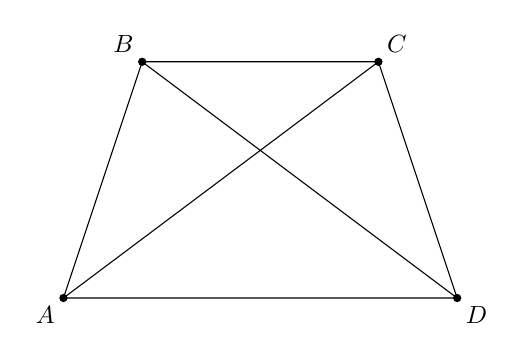
\begin{tikzpicture}[line join =round] 
		\coordinate (A) at (0,0);
		\coordinate (B) at (1,3);
		\coordinate (C) at (4,3);
		\coordinate (D) at (5,0);
		\draw (A)--(B)--(C)--(D)--cycle (D)--(B) (A)--(C);
		\fill (C) node[above right] {$C$} circle (1.5pt);
		\fill (B) node[above left] {$B$} circle (1.5pt);
		\fill (A) node[below left] {$A$} circle (1.5pt);
		\fill (D) node[below right] {$D$} circle (1.5pt);
	\end{tikzpicture}
\end{center}
\loigiai{Hình thang cân $ ABCD $ có hai cạnh bên $ AB=CD $ và hai đường chéo $ BD=AC $. \\Do đó, $ AB+BD=CD+AC>AD $.\\ Vậy 2 điểm $ B, C $ cùng thuộc một elip có hai tiêu điểm là $ A $ và $ D. $ }
\end{bt}

% từ: cau-hoi/lop10/0H9_Phuong_phap_toa_do_trong_mat_phang/0H9-3-8_Bai_toan_thuc_te_PP_toa_do_hoa.tex
\begin{bt}%[0H9V3-8]%[Dự án đề kiểm tra HKII NH22-23-Thy Nguyen Vo Diem]%[THPT Trần Quang Khải]%[ma:f4742cce]
	Có một công viên nhỏ hình tam giác như hình 1. Người ta dự định đặt một cây đèn để chiếu sáng toàn bộ công viên. Để công việc tiến hành thuận lợi, người ta đo đạc và mô phỏng các kích thước công viên và thiết lập một hệ trục $O x y$ như hình 2, khi đó các đỉnh của công viên có tọa độ lần lượt là $A(0;3)$, $B(4;0)$, $C(4{,}7)$. Gọi $I$ là điểm đặt cây đèn sao cho đèn chiếu sáng toàn bộ công viên. Dùng kiến thức đã học, em hãy xác định vị trí chính xác của cây đèn.
	\begin{center}
		\begin{tikzpicture}[line join = round, line cap = round,>=stealth,font=\footnotesize,scale=1]
			\foreach \x/\y/\diem in {0/3/A,4/0/B,4/7/C} \coordinate (\diem) at (\x,\y);
			\draw[thick] (A)--(B)--(C)--cycle;
			\def \kc{0.5}
			\foreach \x in {0,1,2,3} \draw ({-\kc-0.1},\x)--++(0.2,0);
			\foreach \x in {0,1,2,3,4} \draw (\x,{-\kc-0.1})--++(0,0.2);
			\foreach \x in {0,...,7} \draw ({4+\kc-0.1},\x)--++(0.2,0);
			\draw (-\kc,0)--++(0,3) node[midway,left]{$3$ m};
			\draw (0,-\kc)--++(4,0) node[midway,below]{$4$ m};
			\draw ({4+\kc},0)--++(0,7) node[midway,right]{$7$ m};
		\end{tikzpicture}
		\qquad
		\begin{tikzpicture}[line join = round, line cap = round,>=stealth,font=\footnotesize,scale=1]
			\foreach \x/\y/\diem in {0/3/A,4/0/B,4/7/C} \coordinate (\diem) at (\x,\y);
			\def\xt{-1}\def\xp{5}\def\yd{-1}\def\yt{8}
			\draw[->] (\xt,0)--(\xp,0) node[below]{$x$};
			\draw[->] (0,\yd)--(0,\yt) node[left]{$y$};
			\fill (0,0) circle (1.5pt) node[below left]{$O$};
			\draw[thick] (A)--(B)--(C)--cycle;
			\foreach \x in {1,...,4} \draw[thin] (\x,1pt)--(\x,-1pt) node [below] {$\x$};
			\foreach \y in {1,...,7} \draw[thin] (1pt,\y)--(-1pt,\y) node [left] {$\y$};
			\foreach \diem/\goc in {A/0,B/45,C/0} \fill[black](\diem) circle (1pt) ($(\diem)+(\goc:3mm)$) node{$\diem$};
		\end{tikzpicture}
	\end{center}
	\loigiai
	{
		Từ giả thiết, ta có $I$ là tâm đường tròn ngoại tiếp tam giác $ABC$.\\
		Giả sử phương trình đường tròn ngoại tiếp tam giác $ABC$ là
		\[(C)\colon x^2+y^2-2ax-2by+c=0. \]
		với $I(a;b)$ là tâm đường tròn và $a^2+b^2-c>0$.\\
		Ta có $\heva{& A\in (C) \\ & B\in (C) \\ & C\in (C)}\Leftrightarrow \heva{& 0^2+3^2-2a\cdot 0-2b\cdot 3+c=0 \\ & 4^2+0^2-2a\cdot 4-2b\cdot 0+c=0 \\ & 4^2+7^2-2a\cdot 4-2b\cdot 7+c=0}\Leftrightarrow\heva{& a=\dfrac{7}{2} \\ & b=\dfrac{7}{2} \\ & c=12.}$\\
		Vậy $I\left(\dfrac{7}{2};\dfrac{7}{2}\right)$.
	}
\end{bt}

% từ: cau-hoi/lop11/1D1_Ham_so_luong_giac_va_phuong_trinh_luong/1D1-2-2_Xet_dau_gia_tri_luong_giac_Tinh_gia_tri_luong.tex
\begin{ex}%[1D1H2-2]%[ma:b6e567db]
	 Rút gọn biểu thức $M = \cos^4 15^\circ - \sin^4 15^\circ$.
	\choice 
		{$M=1$} 
		{\True  $M=\dfrac{\sqrt{3}}{2}$}
		{$M=\dfrac{1}{4}$} 
		{$M=0$} 
	\loigiai{ 
		Ta có $M = \cos^4 15^\circ  - \sin^4 15^\circ = (\cos^2 15^\circ)^2 - (\sin^2 15^\circ)^2$.\\
		$= (\cos^2 15^\circ  - \sin^2 15^\circ)(\cos^2 15^\circ + \sin^2 15^\circ) = \cos^2 15^\circ - \sin^2 15^\circ = \cos(2 \cdot 15^\circ) = \cos 30^\circ = \dfrac{\sqrt{3}}{2}$.
	 }
\end{ex}

% từ: cau-hoi/lop11/1D1_Ham_so_luong_giac_va_phuong_trinh_luong/1D1-2-3_Bien_doi_rut_gon_bieu_thuc_luong_giac_chung_m.tex
\begin{ex}%[1D1N2-3]%[ma:984549d9]
	Tính  $ A=\sin{390^\circ}-2\sin{1140^\circ}+3\cos{1845^\circ}$
	\choice 
		{\True $\dfrac{1}{2}\left(1+3\sqrt{2}-2\sqrt{3}\right)$} 
		 {$\dfrac{1}{2}\left(1-3\sqrt{2}-2\sqrt{3}\right)$}
		{$\dfrac{1}{2}\left(1+2\sqrt{3}-3\sqrt{2}\right)$} 
		 {$\dfrac{1}{2}\left(1+2\sqrt{3}+3\sqrt{2}\right)$}
	\loigiai{Ta  có
		\allowdisplaybreaks\begin{eqnarray*}
		A&=&\sin 390^\circ-2\sin 1140^\circ +3\cos 1845^\circ \\ 
		&=&\sin\left(2\cdot 180^\circ+30^\circ\right)-2\sin\left(6\cdot  180^\circ+60^\circ\right)+3\cos\left(10\cdot 180^\circ+45^\circ\right)\\
		 &=& \sin 30^\circ -2\sin 60^\circ+3\cos45^\circ\\
		 &=& \dfrac{1}{2}-2\cdot \dfrac{\sqrt{3}}{2}+3\cdot\dfrac{\sqrt{2}}{2}\\
		 &=&\dfrac{1}{2}\left(1-2\sqrt{3}+3\sqrt{2}\right).
	\end{eqnarray*}
} 
\end{ex}

% từ: cau-hoi/lop11/1D1_Ham_so_luong_giac_va_phuong_trinh_luong/1D1-2-4_Cac_goc_luong_giac_co_lien_quan_dac_biet_bu_n.tex
\begin{ex}%[1D1H2-4]%[ma:8ddcb394]
	Rút gọn biểu thức $ A=\dfrac{\sin\left(-234^\circ \right)-\cos216^\circ }{\sin 144^\circ -\cos126^\circ }\cdot \tan36^\circ  $, ta được
	\choice 
		{\True $  A=2$}
		{$ A=-2$} 
		 {$ A=1$}
		{$  A=-1$}
	 \loigiai{
		 Ta có
		\allowdisplaybreaks\begin{eqnarray*}
		A&=&\dfrac{\sin\left(-234^\circ \right)-\cos216^\circ }{\sin 144^\circ -\cos126^\circ }\cdot  \tan36^\circ \\
		&=&\dfrac{-\sin\left(180^\circ+54^\circ\right)-\cos\left(180^\circ +36^\circ \right)}{\sin\left(180^\circ  -36^\circ\right)-\cos\left(90^\circ+36^\circ\right)}\cdot \tan36^\circ\\
		&=&\dfrac{\sin 54^\circ+\cos36^\circ}{\sin 36^\circ+\sin  36^\circ}\cdot \tan 36^\circ\\
		&=&2\cot 36^\circ \cdot  \tan 36^\circ\\
		 &=&2.
	\end{eqnarray*}
 }
\end{ex}

% từ: cau-hoi/lop11/1D1_Ham_so_luong_giac_va_phuong_trinh_luong/1D1-2-4_Cac_goc_luong_giac_co_lien_quan_dac_biet_bu_n.tex
\begin{ex}%[1D1H2-4]%[ma:84e9bd54]
	Giá trị  của biểu thức $A=\dfrac{1}{\tan 368^\circ}+\dfrac{2\sin 2550^\circ \cdot \cos\left(-188^\circ\right)}{2\cos 638^\circ +\cos 98^\circ}$ bằng
	 \choice
		 {$1$}
		 {$ 2$}
		{$-1$} 
		{\True  $0$}
	\loigiai{ 
		Ta  có
		\allowdisplaybreaks\begin{eqnarray*}
		A&=&\dfrac{1}{\tan 368^\circ}+\dfrac{2\sin 2550^\circ \cdot  \cos\left(-188^\circ\right)}{2\cos 638^\circ +\cos 98^\circ}\\
		& =& \dfrac{1}{\tan\left(8^\circ +360^\circ \right)}+\dfrac{2\sin\left(30^\circ+7\cdot  360^\circ\right)\cdot\cos\left(8^\circ+180^\circ\right)}{2\cos\left(-82^\circ+2\cdot 360^\circ\right)+\cos\left(90^\circ+8^\circ\right)}\\
		&=&\dfrac{1}{\tan 8^\circ}+\dfrac{-2\sin 30^\circ\cdot  \cos 8^\circ}{2\cos 82^\circ -\sin 8^\circ}\\
		&=&\dfrac{1}{\tan 8^\circ}-\dfrac{2\sin  30^\circ\cdot \cos 8^\circ}{2\cos\left(90^\circ-8^\circ\right)-\sin 8^\circ}\\
		&=&\dfrac{1}{\tan 8^\circ}-\dfrac{2\sin 30^\circ\cdot \cos 8^\circ}{2\sin 8^\circ-\sin  8^\circ}\\
		 &=&\cot 8^\circ-\dfrac{ \cos 8^\circ}{\sin 8^\circ}\\
		&=&\cot  8^\circ-\cot 8^\circ\\
		 &=&0.
	\end{eqnarray*}
 }
\end{ex}

% từ: cau-hoi/lop11/1D1_Ham_so_luong_giac_va_phuong_trinh_luong/1D1-2-4_Cac_goc_luong_giac_co_lien_quan_dac_biet_bu_n.tex
\begin{ex}%[1D1H2-4]%[ma:265f718e]
	Tính giá trị  của biểu thức
	\begin{align*}
		M=&\cos ^210^\circ+\cos ^220^\circ+\cos ^230^\circ+\cdots+\cos ^2170^\circ+\cos  ^2180^\circ.
	\end{align*}
	 \loigiai{
		Áp dụng công thức $\cos \alpha=\cos \left(180^\circ-\alpha \right)$ và $\cos ^2\alpha+\sin ^2\alpha=1$  ta có
		\begin{eqnarray*}
			M&=&\cos ^210^\circ+\cos ^220^\circ+\cos  ^230^\circ+\cdots+\cos ^2170^\circ+\cos ^2180^\circ\\
			&=&\cos ^210^\circ+\cos ^220^\circ+\cdots+\cos ^280^\circ+\cos ^290^\circ+\cos ^280^\circ+\cdots++\cos ^220^\circ+\cos  ^210^\circ+\cos ^290^\circ\\
			&=&2\left(\cos ^210^\circ+\cos ^220^\circ+\cos ^230^\circ+\cdots+\cos ^280^\circ+\cos  ^290^\circ\right)\\
			 &=&2\left(\sin ^280^\circ+\cdots+\sin ^250^\circ+\cos ^250^\circ+\cdots+\cos ^280^\circ+\cos ^290^\circ\right)=8.
		\end{eqnarray*}
	} 
\end{ex}

% từ: cau-hoi/lop11/1D1_Ham_so_luong_giac_va_phuong_trinh_luong/1D1-2-4_Cac_goc_luong_giac_co_lien_quan_dac_biet_bu_n.tex
\begin{bt}%[1D1V2-4]%[ma:042c9c35]
	Tính giá trị của biểu thức $B=\cos 20^\circ+\cos 40^\circ+\cos 60^\circ  +\cdots+\cos180^\circ$.
	\loigiai{ 
		Ta có  $\cos\left(180^\circ-x\right)=-\cos x\Rightarrow \cos x+\cos\left(180^\circ-x\right)=0$.\\
		$\Rightarrow \heva{&\cos20^\circ+\cos160^\circ=0\\& \cos 40^\circ+\cos140^\circ=0\\&\cos  60^\circ+\cos 120^\circ=0\\& \cos 80^\circ+\cos 100^\circ=0}\Rightarrow B=4.0 +\cos 180^\circ =0-1=-1$.
	 }
\end{bt}

% từ: cau-hoi/lop11/1D1_Ham_so_luong_giac_va_phuong_trinh_luong/1D1-2-4_Cac_goc_luong_giac_co_lien_quan_dac_biet_bu_n.tex
\begin{ex}%[1D1V2-4]%[ma:e6b34706]
	Tính giá trị của biểu thức $B=\cos  20^\circ+\cos 40^\circ+\cos 60^\circ +\cdots+\cos180^\circ$.
	 \loigiai{
		Ta có $\cos\left(180^\circ-x\right)=-\cos x\Rightarrow \cos  x+\cos\left(180^\circ-x\right)=0$.\\
		$\Rightarrow \heva{&\cos20^\circ+\cos160^\circ=0\\& \cos 40^\circ+\cos140^\circ=0\\&\cos 60^\circ+\cos 120^\circ=0\\& \cos 80^\circ+\cos 100^\circ=0}\Rightarrow B=4.0 +\cos  180^\circ =0-1=-1$.
	} 
\end{ex}

% từ: cau-hoi/lop11/1D1_Ham_so_luong_giac_va_phuong_trinh_luong/1D1-2-4_Cac_goc_luong_giac_co_lien_quan_dac_biet_bu_n.tex
\begin{ex}%[1D1H2-4]%[ma:86974c5c]
	 Biểu thức $ A=\cos20^{\circ} +\cos40^{\circ} + \cos60^{\circ}+\cdots+\cos160^{\circ}+\cos180^{\circ}$ có giá trị bằng\\
	\shortans{-1} 
	 \loigiai{Ta có
	\begin{eqnarray*}
		A&=&(\cos20^{\circ}+\cos160^{\circ})+(\cos40^{\circ}+\cos140^{\circ})+\cdots+(\cos80^{\circ}+\cos100^{\circ})+\cos180^{\circ}\\ 
		 &=&(\cos20^{\circ}-\cos20^{\circ})+(\cos40^{\circ}-\cos40^{\circ})+\cdots+(\cos80^{\circ}-\cos80^{\circ})+\cos180^{\circ} \\
		 &=& 0+ 0 +\cdots+ 0 -1\\
		 &=& -1.
	\end{eqnarray*}
	} 
\end{ex}

% từ: cau-hoi/lop11/1D1_Ham_so_luong_giac_va_phuong_trinh_luong/1D1-2-5_Toan_thuc_te_ap_dung_gia_tri_cua_mot_goc_luon.tex
\begin{bt}%[1D1V2-5]%[ma:b532365c]
% nguon: Archive/SP_KhoLatex/ID6_old/1K1-ot.tex #3778
%[Dự án 2 - TLDH - TeamTeXHoa - Quang Ngô]
    Khi một tia sáng truyền từ ông khí vào mặt nước thì một phần tia sáng bị phản xạ trên bề mặt, phần còn lại bị khúc xạ như trong Hình. Góc tới $i$ liên hệ với góc khúc xạ $r$ bởi Định luật khúc xạ ánh $\dfrac{\sin i}{\sin r}=\dfrac{n_2}{n_1}. $
    \begin{center}
        \begin{tikzpicture}[line join = round, line cap = round, >=stealth, font=\footnotesize, scale=1]
            
            \path 
            (-1,0) coordinate (A)
            (5,0) coordinate (B)
            (2,0) coordinate (C)
            (-1,2) coordinate (D)
            (5,2) coordinate (E)
            (2,3) coordinate (F)
            (2,-3) coordinate (G)
            (4,-3) coordinate (H)
            ;
            \fill[color=blue!20] (A)--(B)--(5,-3.2)--(-1,-3.2)--(A);
            \draw
            (A)--(B)
            ($(C)!.7!(H)$)--(H)node[right]{$R$}
            ($(D)!.3!(C)$)--(C)node[below left]{$I$}
            ($(C)!.7!(E)$)--(E)node[above]{$S'$}
            pic[draw,black,angle radius=0.3cm] {angle = F--C--D}
            (C)++(120:.5)node{$i$}
            pic[draw,black,angle radius=0.4cm] {angle = E--C--F}
            (C)++(60:.6)node{$i'$}
            pic[draw,black,angle radius=0.3cm] {angle = G--C--H}
            pic[draw,black,angle radius=0.4cm] {angle = G--C--H}
            (C)++(-70:.6)node{$r$}
            ;
            \draw[->]
            (C)--($(C)!.7!(H)$);
            \draw[->]
            (D)node[above]{$S$}--($(D)!.3!(C)$);
            \draw[->]           
            (C)--($(C)!.7!(E)$);
            \draw[dashed] (F)node[left]{$N$}--(G)node[left]{$N'$};
            \draw 
            (A)++(60:.5) circle (2mm)node{$1$}
            (A)++(-60:.5) circle (2mm)node{$2$}
            ;
        \end{tikzpicture}
    \end{center}
    Ở đây, $n_1$ và $n_2$ tương ứng là chiết suất của môi trường 1 (không khí) và môi trường 2 (nước). Cho biết góc tới $i=50^\circ$, hãy tính góc khúc xạ, biết rằng chiết suất của không khí bằng 1 còn chiết suất của nước là $1{,}33$.
    \loigiai{
        Theo bài ra ta có: $ i=50^\circ$, $n_1=1$, $n_2=1{,}33$, thay vào $\dfrac{\sin i}{\sin r}=\dfrac{n_2}{n_1}$ ta được:\\
        $\dfrac{\sin{50}^\circ}{\sin r}=\dfrac{1{,}33}{1}$ (đk $\sin r\neq 0$)\\
        $\Rightarrow \sin r=\dfrac{\sin50^\circ}{1{,}33}$$\Leftrightarrow \sin r\approx 0{,}57597$ (thỏa mãn điều kiện)\\
        $\Leftrightarrow \sin r\approx \sin\left(35^\circ10^\prime\right)$\\
        $\Leftrightarrow \hoac{
            &r\approx 35^\circ10^\prime+k360^\circ \\
            &r\approx 180^\circ-35^\circ10^\prime+k360^\circ 
        }\left(k\in \mathbb{Z}\right) \\
        \Leftrightarrow \hoac{
            &r\approx 35^\circ10^\prime+k360^\circ \\
            &r\approx 144^\circ50^\prime+k360^\circ 
        }\left(k\in \mathbb{Z}\right)$ \\
        Mà $0^\circ<r<90^\circ$ nên $r\approx 35^\circ10^\prime$.\\
        Vậy góc khúc xạ $r\approx 35^\circ10^\prime.$
    }
\end{bt}

% từ: cau-hoi/lop11/1D1_Ham_so_luong_giac_va_phuong_trinh_luong/1D1-2-5_Toan_thuc_te_ap_dung_gia_tri_cua_mot_goc_luon.tex
\begin{bt}%[1D1H2-5]%[ma:5527179a]
% nguon: Archive/2024/TOAN_11_XE/TOAN_11_XE/data4/11C1/KNTT-1.OTC.tex #1112
%[Tex hóa SGK CD-CT,T12/22, TVN-006]
\immini{
Khi một tia sáng truyền từ không khí vào mặt nước thì một phần tia sáng bị phản xạ trên bề mặt, phần còn lại bị khúc xạ như hình bên. Góc tới $i$ liên hệ với góc khúc xạ $r$ bởi Định luật khúc xạ ánh sáng
$$\dfrac{\sin i}{\sin r}=\dfrac{n_2}{n_1}.$$
Ở đây, $n_1$ và $n_2$ tương ứng với chiết suất của môi trường $1$ (không khí) và môi trường $2$ (nước). Cho biết góc tới $i=50^\circ$, hãy tính góc khúc xạ, biết rằng chiết suất của không khí bằng $1$ còn chiết suất của nước là $1{,}33$.
}
{
	\begin{tikzpicture}[>=stealth,line join=round,line cap=round,font=\footnotesize,scale=.7]
	\path
	(0,0)coordinate(I)++(90:3)coordinate(N)++(-90:6)coordinate(N')
	(I)++(0:3)coordinate(B)++(180:6)coordinate(A)
	(I)++(30:3)coordinate(S')
	(I)++(150:3)coordinate(S)
	(I)++(-55:3)coordinate(R)
	;
	\fill[cyan!20!](-3,-3)rectangle(3,0)
	;
	\draw (A)--(B)
	;
	\draw[dashed](N)--(N')
	;
	\draw[->,midway](S)--(I)
	;
	\draw[->](I)--(S')
	;
	\draw[->](I)--(R)
	;
	\foreach \p/\r in {N/180,N'/180,S/160,S'/90,R/0,I/-135}
	\fill (\p) node[shift={(\r:3mm)}]{$\p$}
	;
	\draw pic[angle radius=3mm,draw=red,fill=green!50,"$i$",angle eccentricity=1.5] {angle = N--I--S}
	;
	\draw pic[angle radius=4mm,draw=orange,fill=orange!50,"$i'$",angle eccentricity=1.5] {angle = S'--I--N}
	;
	\draw pic[angle radius=4mm,draw=blue,fill=blue!50,"$r$",angle eccentricity=1.5] {angle = N'--I--R}
	;
	\draw (-2.5,.5)circle(7pt)node{$1$}
		(-2.5,-.5)circle(8pt)node{$2$}
		;	
\end{tikzpicture}
}
\loigiai{
Ta có $\dfrac{\sin i}{\sin r}=\dfrac{n_2}{n_1}\Leftrightarrow \dfrac{\sin 50^\circ}{\sin r}=\dfrac{1{,}33}{1}\Leftrightarrow \sin r=\dfrac{\sin 50^\circ}{1{,}33}\Rightarrow r\approx 35{,}17^\circ$.
}
\end{bt}

% từ: cau-hoi/lop11/1D1_Ham_so_luong_giac_va_phuong_trinh_luong/1D1-3-2_Ap_dung_cong_thuc_cong.tex
\begin{ex}%[1D1H3-2]%[ma:a9d140ad]
	Rút gọn biểu thức $\cos 54^\circ  \cos 4^\circ - \cos 36^\circ \cos 86^\circ$, ta được
	\choice 
		 {$\cos 50^\circ$}
		{\True  $\cos 58^\circ$}
		{$\sin 50^\circ$} 
		 {$\sin 58^\circ$}
	 \loigiai{
		Ta có $\cos 54^\circ \cos 4^\circ - \cos 36^\circ \cos  86^\circ = \cos 54^\circ \cos 4^\circ - \sin 54^\circ \sin 4^\circ= \cos (54^\circ + 4^\circ) = \cos 58^\circ$.
	 }
\end{ex}

% từ: cau-hoi/lop11/1D1_Ham_so_luong_giac_va_phuong_trinh_luong/1D1-3-3_Ap_dung_cong_thuc_nhan_doi_ha_bac.tex
\begin{ex}%[1D1H3-3]%[ma:6ce93a6f]
	Tính giá trị của $M=\cos  ^415^\circ-\sin ^415^\circ $.
	\choice 
		{$M=1$} 
		{\True  $M=\dfrac{\sqrt{3}}{2}$}
		{$M=\dfrac{1}{4}$} 
		{$M=0$} 
	\loigiai{ 
		\begin{eqnarray*}
			 M&=&\cos ^415^\circ-\sin ^415^\circ\\
			&=&\left(\cos ^215^\circ \right)^2-\left(\sin  ^215^\circ \right)^2\\
			&=&\left(\cos ^215^\circ-\sin ^215^\circ \right)\left(\cos ^215^\circ+\sin ^215^\circ \right) 
			\\ &=&\cos ^215^\circ-\sin ^215^\circ 
			 \\ &=&\cos \left(2\cdot 15^\circ \right)\\
			&=&  \cos 30^\circ=\dfrac{\sqrt{3}}{2}.
		\end{eqnarray*}
	} 
\end{ex}

% từ: cau-hoi/lop11/1D1_Ham_so_luong_giac_va_phuong_trinh_luong/1D1-3-4_Ap_dung_cong_thuc_bien_doi_tich_tong.tex
\begin{ex}%[1D1H3-4]%[ma:c1355ba1]
	Tính giá trị biểu thức $P=\sin 30^\circ \cdot \cos 60^\circ+\sin  60^\circ \cdot \cos 30^\circ$.
	 \choice
		{\True  $P=1$}
		 {$P=0$}
		{$P=\sqrt  {3}$}
		{$P=-\sqrt {3}$} 
	\loigiai{Ta có $P=\sin  \left(30^\circ+60^\circ\right)=\sin 90^\circ=1$.
	} 
\end{ex}

% từ: cau-hoi/lop11/1D1_Ham_so_luong_giac_va_phuong_trinh_luong/1D1-3-5_Ket_hop_nhieu_cong_thuc_luong_giac.tex
\begin{ex}%[1D1V3-5]%[ma:ba300da3]
	Kết quả  nào sau đây \textbf{SAI}?
	\choice 
		{\True  $\sin 33^\circ+\cos 60^\circ=\cos 3^\circ $}
		{$\dfrac{\sin 9^\circ}{\sin  48^\circ}=\dfrac{\sin 12^\circ}{\sin 81^\circ}$}
		{$\cos 20^\circ+2\sin  ^255^\circ=1+\sqrt 2\sin 65^\circ $}
		 {$\dfrac{1}{\cos 290^\circ}+\dfrac{1}{\sqrt 3\sin 250^\circ}=\dfrac{4}{\sqrt 3}$}
	\loigiai{ 
		Xét 
		\allowdisplaybreaks 
		\begin{eqnarray*}
			& &  \dfrac{\sin 9^\circ}{\sin 48^\circ}=\dfrac{\sin 12^\circ}{\sin 81^\circ}\\
			&\Leftrightarrow& \sin 9^\circ \cdot \sin  81^\circ-\sin 12^\circ \cdot\sin 48^\circ=0\\
			&\Leftrightarrow&  \dfrac{1}{2}\left(\cos 72^\circ-\cos 90^\circ\right)-\dfrac{1}{2}\left(\cos 36^\circ-\cos 60^\circ\right)=0\\
			&\Leftrightarrow& 2\cos 72^\circ-2\cos 36^\circ+1=0\\ 
			&\Leftrightarrow& 4\cos ^236^\circ-2\cos  36^\circ-1=0.
		\end{eqnarray*}
		Vậy $\dfrac{\sin 9^\circ}{\sin 48^\circ}=\dfrac{\sin 12^\circ}{\sin  81^\circ}$ đúng.\\
		Tương tự chứng minh  được các đẳng thức $\cos 20^\circ+2\sin ^255^\circ=1+\sqrt 2\sin 65^\circ $; \break
		 $\dfrac{1}{\cos 290^\circ}+\dfrac{1}{\sqrt 3\sin 250^\circ}=\dfrac{4}{\sqrt 3}$ đúng.\\
		Suy ra đẳng  thức sai là $\sin 33^\circ+\cos 60^\circ=\cos 3^\circ $.
	} 
\end{ex}

% từ: cau-hoi/lop11/1D1_Ham_so_luong_giac_va_phuong_trinh_luong/1D1-3-5_Ket_hop_nhieu_cong_thuc_luong_giac.tex
\begin{ex}%[1D1V3-5]%[ma:b04beafc]
	Tính giá trị của  biểu thức $M=\cos^6{15^{\circ}}-\sin^6{15^{\circ}}$ (làm tròn đến hàng phần trăm).
	 \shortans{0,81}
	\loigiai{ 
	Ta  có
	$$\begin{array}{l}
	 \cos ^6\alpha-\sin ^6\alpha\\
	=\left(\cos^2\alpha-\sin^2\alpha\right)\left(\cos^4\alpha+\cos^2\alpha  \cdot\sin^2\alpha+\sin^4\alpha\right)\\
	=\cos  2\alpha \cdot\left[\left(\cos^2\alpha+\sin^2\alpha\right)^2-\cos^2\alpha \cdot\sin^2\alpha\right]\\
	 =\cos 2\alpha \cdot\left(1-\dfrac{1}{4}{\sin^2}2\alpha\right).
\end{array}$$
Vậy $ M=\cos{30^{\circ}}\cdot\left(1-\dfrac{1}{4}{\sin^2}{30^{\circ}}\right)=\dfrac{\sqrt 3}{2}\cdot\left(1-\dfrac{1}{4}\cdot\dfrac{1}{4}\right)=\dfrac{15\sqrt 3}{32}\approx  0{,}81$.
} 
\end{ex}

% từ: cau-hoi/lop11/1D1_Ham_so_luong_giac_va_phuong_trinh_luong/1D1-4-4_Xet_tinh_chan_le.tex
\begin{bt}%[1D1H4-4]%[ma:4f309c5b]
% nguon: Archive/SP_KhoLatex/ID6_old/1K1-3.tex #3540
%[Dự án 1 - TLDH - TeamTeXHoa - Lê Minh Cường]
	Xét tính chẵn, lẻ của các hàm số sau:
	\begin{listEX}[2]
		\item $y=2 \sin x+3$;
		\item $y=\sin x+\cos x$.
	\end{listEX}
	\loigiai{
		\begin{listEX}[1]
			\item  TXĐ $\mathscr{D}=\mathbb{R}$.\\
			Suy ra $\forall x \in \mathscr{D} \Rightarrow -x \in \mathscr{D}$.\\
			Ta có
			$f\left(-\dfrac{\pi}{2}\right)=2 \sin \left(-\dfrac{\pi}{2}\right)+3=1 ; f\left(\dfrac{\pi}{2}\right)=2 \sin \left(\dfrac{\pi}{2}\right)+3=5$.\\
			Nhận thấy
			$\heva{&f\left(-\dfrac{\pi}{2}\right) \neq f\left(\dfrac{\pi}{2}\right)\\ & f\left(-\dfrac{\pi}{2}\right) \neq-f\left(\frac{\pi}{2}\right).}$\\
			Do đó hàm số không chẵn không lẻ.
			\item  TXĐ $\mathscr{D}=\mathbb{R}$.\\
			Suy ra $\forall x \in \mathscr{D} \Rightarrow -x \in \mathscr{D}$.\\
			Ta có $y=\sin x+\cos x=\sqrt{2} \sin \left(x+\dfrac{\pi}{4}\right)$\\
			$f\left(-\dfrac{\pi}{4}\right)=\sqrt{2} \sin \left(-\dfrac{\pi}{4}+\dfrac{\pi}{4}\right)=0 ; f\left(\dfrac{\pi}{4}\right)=\sqrt{2} \sin \left(\dfrac{\pi}{4}+\dfrac{\pi}{4}\right)=\sqrt{2}$.\\			
			Nhận thấy $\heva{&f\left(-\dfrac{\pi}{4}\right) \neq f\left(\dfrac{\pi}{4}\right)\\ & f\left(-\dfrac{\pi}{4}\right) \neq-f\left(\frac{\pi}{4}\right).}$\\			
			Do đó hàm số không chẵn không lẻ.
		\end{listEX}
	}
\end{bt}

% từ: cau-hoi/lop11/1D1_Ham_so_luong_giac_va_phuong_trinh_luong/1D1-4-8_Toan_thuc_te_ap_dung_ham_so_luong_giac.tex
\begin{ex}%[1D1V4-8]%[ma:13d69c2e]
	\immini[thm]{ 
	Một cái guồng nước có vành kim loại ngoài cùng là một đường tròn tâm $O$, bán kính là $4$ m. Xét chất điểm $M$ thuộc đường tròn đó và góc $\alpha=(OA, OM)$. Giả sử mực nước lúc đang xét là tiếp xúc với đường tròn $(O; 4)$ và guồng nước quay  theo chiều dương (ngược chiều kim đồng hồ).
	Biết rằng guồng nước quay hết một vòng sau $40$ giây ($t=0$ giây khi điểm $M$ trùng $A$). Hỏi thời điểm nào (trong $1$ vòng quay đầu tiên) thì  điểm $M$ ở vị trí cao nhất so với mặt nước?}{
	\begin{tikzpicture}[line join = round,line cap = round,>=stealth,font=\footnotesize,scale=.5]
			\foreach  \i in {0,1,...,40}
			 \draw[gray] (0,0)--(\i*10:5);
			 \draw[line width=3pt,green!50!black] (0,0) circle (5cm);
			 \draw[gray] (0,0) circle (4.5cm);
			 \draw[gray] (0,0) circle (4cm);
			\draw[gray] (0,0)  circle (3.5cm);
			\draw[green!60!black,line width=1pt]  (5,0) coordinate (A)--(0,0) coordinate (O)--++(60:5) coordinate (M) node[above right]{$M$};
			\draw[->] pic [draw,angle radius = 9 mm] {angle = A--O--M}; 
			\draw[red] (.7,.45) node{$\alpha$}; 
			\fill  (M) circle (3pt);
			\fill (0,0)  node[below left]{$O$} circle (3pt);
			\fill (5,0) node[above right] {$A$} circle (2pt); 
			 \draw[->] (-6,0)--(6,0) node[below]{$x$};
			 \draw[->] (0,-6)--(0,6) node[right]{$y$};
		\end{tikzpicture}
	 }
	 \shortans{10}
	 \loigiai{
		Ta có $h(x)=4+4 \sin \alpha$.  \\
		Khi $M$ ở vị trí cao nhất so với mặt nước (tức là $h(x)=8$) thì $\sin \alpha=1 \Rightarrow  \alpha=\dfrac{\pi}{2}$ (vì chỉ xét $1$ vòng quay đầu tiên). \\
		Thời gian thực hiện của guồng nước là  $t=\dfrac{\dfrac{\pi}{2}\cdot 40}{2 \pi}=10$ (giây).
	} 
\end{ex}

% từ: cau-hoi/lop11/1D1_Ham_so_luong_giac_va_phuong_trinh_luong/1D1-5-3_Phuong_trinh_co_ban_dung_Radian.tex
\begin{bt}%[1D1H5-3]%[ma:da76ff99]
% nguon: Archive/2024/SP-K10-K11-LyVanHoang_TVN-023/11. C1-LuongGiac-lvhoang_TVN-023/dataC1K11/Chuong1-Bai4-Dang3-PhuongTrinhCBDungRadian.tex #1630
[Mức H, Cánh Diều]%[BG Toán 11 CT2025, Quan Ón]
	Giải các phương trình
	\begin{multicols}{3}
		\begin{enumerate}
			\item $\sin x=-\dfrac{1}{2}$;
			\item $\sin x=\dfrac{\sqrt{2}}{2}$;
			\item $\cos x=\dfrac{\sqrt{3}}{2}$;
			\item $\cos x=-\dfrac{\sqrt{2}}{2}$;
			\item $\cos x=-\dfrac{1}{2}$;
			\item $\cos3x=\cos\left(x+\dfrac{\pi}{3}\right)$;
			\item $\tan x=\dfrac{1}{\sqrt{3}}$;
			\item $\tan x=-1$;
			\item $\cot2x=-\sqrt{3}$.
		\end{enumerate}
	\end{multicols}
	\loigiai{
		\begin{enumerate}
			\item Do $\sin\left(-\dfrac{\pi}{6}\right)=-\dfrac{1}{2}$ nên $$\sin x=\sin\left(-\dfrac{\pi}{6}\right)\Leftrightarrow\hoac{&x=-\dfrac{\pi}{6}+k2\pi\\&x=\pi-\left(-\dfrac{\pi}{6}\right)+k2\pi}\Leftrightarrow\hoac{&x=-\dfrac{\pi}{6}+k2\pi\\&x=\dfrac{7\pi}{6}+k2\pi}\,(k\in\mathbb{Z}).$$
			\item Do $\sin\dfrac{\pi}{4}=\dfrac{\sqrt{2}}{2}$ nên $$\sin x=\sin\dfrac{\pi}{4}\Leftrightarrow\hoac{&x=\dfrac{\pi}{4}+k2\pi\\&x=\pi-\dfrac{\pi}{4}+k2\pi}\Leftrightarrow\hoac{&x=\dfrac{\pi}{4}+k2\pi\\&x=\dfrac{3\pi}{4}+k2\pi}\,(k\in\mathbb{Z}).$$
			\item $\cos x=\dfrac{\sqrt{3}}{2}\Leftrightarrow\cos x=\cos\dfrac{\pi}{6}\Leftrightarrow x=\pm\dfrac{\pi}{6}+k2\pi,\,(k\in\mathbb{Z})$.
			\item $\cos x=-\dfrac{\sqrt{2}}{2}\Leftrightarrow \cos x=\cos\dfrac{3\pi}{4}\Leftrightarrow x=\pm\dfrac{3\pi}{4}+k2\pi,\,(k\in\mathbb{Z})$.
			\item $\cos x=-\dfrac{1}{2}\Leftrightarrow\cos x=\cos\dfrac{2\pi}{3}\Leftrightarrow x=\pm\dfrac{2\pi}{3}+k2\pi,\,(k\in\mathbb{Z})$.
			\item $\cos3x=\cos\left(x+\dfrac{\pi}{3}\right)\Leftrightarrow\hoac{&3x=x+\dfrac{\pi}{3}+k2\pi\\&3x=-x-\dfrac{\pi}{3}+k2\pi}\Leftrightarrow\hoac{&x=\dfrac{\pi}{6}+k\pi\\&x=-\dfrac{\pi}{12}+\dfrac{k\pi}{2}},\,(k\in\mathbb{Z})$.
			\item $\tan x=\dfrac{1}{\sqrt{3}}\Leftrightarrow\tan x=\tan\dfrac{\pi}{6}\Leftrightarrow x=\dfrac{\pi}{6}+k\pi,\,(k\in\mathbb{Z})$.
			\item $\tan x=-1\Leftrightarrow\tan x=\tan\left(-\dfrac{\pi}{4}\right)\Leftrightarrow x=-\dfrac{\pi}{4}+k\pi,\,(k\in\mathbb{Z})$.
			\item $\cot2x=-\sqrt{3}\Leftrightarrow\cot2x=\cot\left(-\dfrac{\pi}{6}\right)\Leftrightarrow x=-\dfrac{\pi}{6}+k\pi,\,(k\in\mathbb{Z})$.
	\end{enumerate}}
\end{bt}

% từ: cau-hoi/lop11/1D1_Ham_so_luong_giac_va_phuong_trinh_luong/1D1-5-3_Phuong_trinh_co_ban_dung_Radian.tex
\begin{bt}%[1D1H5-3]%[ma:3c6efab6]
% nguon: Archive/SP_KhoLatex/ID6_old/11-OT-PTLuongGiacCoBan.tex #3093
%[ĐGNL-ĐGTD-2022, Tran Tony]
	Giải phương trình $\cos 3x = \dfrac{1}{3}$.
	\loigiai{Ta có  $\cos 3x = \dfrac{1}{3}\Leftrightarrow \hoac{&3x=\arccos\dfrac{1}{3}+k2\pi\\&3x=-\arccos\dfrac{1}{3}+k2\pi}\Leftrightarrow \hoac{&x=\dfrac{1}{3}\arccos\dfrac{1}{3}+\dfrac{k2\pi}{3}\\&x=\dfrac{1}{3}\arccos\dfrac{1}{3}+\dfrac{k2\pi}{3}}, (k\in \mathbb{Z}).$
	}	
\end{bt}

% từ: cau-hoi/lop11/1D1_Ham_so_luong_giac_va_phuong_trinh_luong/1D1-5-4_Phuong_trinh_co_ban_dung_Do.tex
\begin{bt}%[1D1H5-4]%[ma:337ac33b]
% nguon: Archive/2024/TOAN_11_XE/TOAN_11_XE/data4/11C1/KNTT-1.4.tex #1075
%[Tex hóa SGK 11, KNTT]
	Giải phương trình $\sin 2x  = \sin (60^{\circ} - 3x)$.
	\loigiai{
Ta có 
\begin{align*}
\sin 2x = \sin (60^{\circ}-3x) & \Leftrightarrow \hoac{& 2x = 60^{\circ}-3x + k360^{\circ} \\ & 2x = 180^{\circ} - (60^{\circ}-3x) + k360^{\circ}}
		\Leftrightarrow \hoac{& 5x = 60^{\circ} + k360^{\circ} \\ & -x = 120^{\circ} + k360^{\circ}} \\
		&\Leftrightarrow \hoac{& x = 12^{\circ} + k72^{\circ} \\ & x = -120^{\circ} - k360^{\circ}} \quad (k \in \mathbb{Z}).
\end{align*}
	}
\end{bt}

% từ: cau-hoi/lop11/1D1_Ham_so_luong_giac_va_phuong_trinh_luong/1D1-5-5_Phuong_trinh_dua_ve_dang_co_ban.tex
\begin{bt}%[1D1H5-5]%[ma:deccbfed]
% nguon: Archive/2024/SP-K10-K11-LyVanHoang_TVN-023/11. C1-LuongGiac-lvhoang_TVN-023/dataC1K11/Chuong1-Bai4-Dang5-Phuongtrinhduavecoban.tex #2032
%[Bài giảng 11, Trần Tony]
	Giải các phương trình sau
	\begin{listEX}[2]
		\item $\dfrac{1 + \cos 4x - 2 \cos 2x}{\sin \left( x + \dfrac{\pi}{4} \right) \sin 2x} = 0$.
		\item $\dfrac{4\sin^22x+6\sin^2x-9-3\cos2x}{\cos x\left(\sin x-\dfrac{\sqrt{3}}{2}\right)}=0$.
	\end{listEX}
	\loigiai{
		\begin{enumerate}[a)]
			\item	Điều kiện xác định:\\
			$\sin \left( x + \dfrac{\pi}{4}\right) \sin 2x \ne 0 \Leftrightarrow \heva{&x \ne -\dfrac{\pi}{4}+k\pi \\& x \ne \dfrac{l\pi}{2}}$, với $k, l \in \mathbb{Z}$.\\
			Phương trình 
			\begin{eqnarray*}
				&&\dfrac{1 + \cos 4x - 2 \cos 2x}{\sin \left( x + \dfrac{\pi}{4}\right) \sin 2x} = 0
				\\&\Leftrightarrow& 2 \cos^2 2x - 2 \cos 2x = 0
				\\&\Leftrightarrow& \hoac{&\cos 2x = 0 \\& \cos 2x = 1 \text{ (loại)}}
				\\&\Leftrightarrow& x = \dfrac{\pi}{4} + \dfrac{k\pi}{2}	
			\end{eqnarray*}
			So với điều kiện xác định ở trên, ta có nghiệm của phương trình đã cho là $x = \dfrac{\pi}{4} + k\pi, k \in \mathbb{Z}$.
			\item Điều kiện:$\heva{&\cos x\ne0\\&\sin x\ne\dfrac{\sqrt{3}}{2}}\Leftrightarrow\heva{&x\ne\dfrac{\pi}{2}+k\pi\\&x\ne\dfrac{\pi}{3}+k\pi\\&x\ne\dfrac{2\pi}{3}+k\pi}$ \\
			Phương trình $\Leftrightarrow 4(1-\cos^22x)+3(1-\cos2x)-9-3\cos2x=0$\\
			$\Leftrightarrow4\cos^22x+6\cos2x+2=0\Leftrightarrow\hoac{&\cos2x=-1\\&\cos2x=-\dfrac{1}{2}}\Leftrightarrow\hoac{&x=\dfrac{\pi}{2}+k\pi\\&x=\pm\dfrac{\pi}{3}+k\pi}$ \\
			So điều kiện, nghiệm phương trình là $x=\dfrac{4\pi}{3}+k2\pi$ và $ x=-\dfrac{\pi}{3}+k2\pi$ với $k\in\mathbb{Z}$.
		\end{enumerate}
	}
\end{bt}

% từ: cau-hoi/lop11/1D1_Ham_so_luong_giac_va_phuong_trinh_luong/1D1-5-5_Phuong_trinh_dua_ve_dang_co_ban.tex
\begin{bt}%[1D1V5-5]%[ma:ba22bf93]
% nguon: Archive/SP_KhoLatex/ID6_old/1K1-4-5.tex #3327
%[DCHT Toán 11 - KNTT -Thọ Bùi] 
	Giải phương trình: $\sin^4\dfrac{x}{2}+\cos^4 \dfrac{x}{2}=\dfrac{1}{2}$.
	\loigiai{ Ta có:
		\allowdisplaybreaks
		\begin{eqnarray*}
			\sin^4\dfrac{x}{2}+\cos^4 \dfrac{x}{2}=\dfrac{1}{2}
			&\Leftrightarrow&\left(\sin^2\dfrac{x}{2}+\cos^2\dfrac{x}{2}\right)^2-2\sin^2\dfrac{x}{2}\cos^2\dfrac{x}{2}=\dfrac{1}{2}\\
			&\Leftrightarrow&1-\dfrac{1}{2}\sin^2x=\dfrac{1}{2}\\
			&\Leftrightarrow&\sin^2 x=1\\
			&\Leftrightarrow&\cos x=0\\
			&\Leftrightarrow&x=\dfrac{\pi}{2}+k\pi, \left(k\in \mathbb{Z}\right).
		\end{eqnarray*}
		
	}
\end{bt}

% từ: cau-hoi/lop11/1D1_Ham_so_luong_giac_va_phuong_trinh_luong/1D1-5-6_Toan_thuc_te_ap_dung_phuong_trinh_luong_giac.tex
\begin{ex}%[1D1V5-6]%[1D1C5-6]%[ma:9ec19cc4]
	Một cây cầu có dạng cung $OA$ của đồ thị hàm số $y=4{,}8\sin\dfrac{x}{9}$ và được mô tả trong hệ trục  tọa độ với đơn vị trục là mét như ở hình dưới đây:
	\begin{center}
		\begin{tikzpicture}[scale=1,>=stealth,font=\footnotesize,line join=round,line cap=round,x=4mm,y=5mm]
				\def\xmin{-1.5} \def\xmax{30}  \def\ymin{-1.5} \def\ymax{6}
				\draw[->] (\xmin,0)--(\xmax,0) node  [below]{$x$};
				\draw[->] (0,\ymin)--(0,\ymax)  node [right]{$y$};
				\node at (0,0)  [below left]{$O$};
				 \node at (9*pi,0) [below]{$A$};
				\clip (\xmin+0.1,\ymin+0.1) rectangle (\xmax-0.1,\ymax-0.1); 
				 \draw[smooth,samples=400,domain=0:28.3] plot (\x,{4.8*sin (\x/9 r)});
				\draw[fill,black] (0,0) circle  (1pt)
					 (9*pi,0) circle (1pt);
			\end{tikzpicture}
	\end{center}
	\begin{enumerate}
		\item Giả sử chiều rộng của con sông là độ dài đoạn thẳng  $OA$. Tìm chiều rộng đó (Làm tròn kết quả đến hàng phần mười).
		\item Một sà lan chở khối hàng hóa được xếp thành hình hộp chữ nhật với độ cao $3{,}6$ m so với  mực nước sông sao cho sà lan có thể đi qua được gầm cầu. Chứng minh rằng chiều rộng của khối hàng hóa đó phải nhỏ hơn $13{,}1$ m.
		\item Một sà lan khác cũng chở khối hàng hóa được xếp thành hình hộp chữ nhật với chiều rộng của khối hàng hóa đó là $9$ m sao cho sà lan có thể đi qua được gầm cầu. Chứng minh rằng chiều cao của khối hàng hóa đó phải nhỏ hơn $4{,}3$ m. 
	\end{enumerate}
	 \loigiai{\allowdisplaybreaks
		\begin{enumerate}
			\item Giải  phương trình
			\begin{align*}
				y=0 \Leftrightarrow  4{,}8\sin\dfrac{x}{9}=0 \Leftrightarrow \sin\dfrac{x}{9}=0 \Leftrightarrow \dfrac{x}{9}=k\pi \Leftrightarrow x=k9\pi \left( k\in \mathbb{Z} \right).
			\end{align*}
			 Do đó đồ thị cắt trục $Ox$ tại các điểm có hoành độ $0;9\pi; 18\pi; \ldots$.\\
			Vì  thế $A(9\pi;0)$ nên chiều rộng của con sông là $OA=9\pi \approx 28{,}3$ m.
			\item Xét đường  thẳng $y=3{,}6$.\\
			Ta có $y=4{,}8\sin\dfrac{x}{9} \le 4{,}8$ nên đường thẳng $y=3{,}6$ cắt một phần đồ thị của hàm số $y=4{,}8\sin\dfrac{x}{9}$ tại hai  điểm $M\left(x_1;3{,}6\right)$, $N\left(x_2;3{,}6\right)$.\\
			Giải phương trình $4{,}8\sin\dfrac{x}{9}=3{,}6 \Leftrightarrow \sin\dfrac{x}{9} =\dfrac{3}{4}\  (1)$. \\
			 Gọi $x_1$, $x_2$ là hai nghiệm dương nhỏ nhất của $(1)$.\\
			Vì $-1\le \dfrac{3}{4}\le 1$ nên tồn tại một số $\alpha \in \left[-\dfrac{\pi}{2};\dfrac{\pi}{2}\right]$ sao cho $\sin\alpha=\dfrac{3}{4}$.\\ 
			 Ta có $\sin\dfrac{x}{9}=\sin\alpha \Leftrightarrow $
			 $\hoac{&\dfrac{x}{9}=\alpha+k2\pi\\&\dfrac{x}{9}=\pi-\alpha+k2\pi} \Leftrightarrow \hoac{&x=9\alpha+k18\pi\\&x=9\pi-9\alpha+k18\pi.}$\\
			 Do $x_1; x_2\in (0;9\pi)$ nên $x_1 \approx 9\alpha \approx 7{,}6325$; $x_1 \approx 9\pi-9\alpha \approx 20{,}6418$ nên $x_2-x_1<13{,}1$.\\
			Vậy chiều  rộng của khối hàng hoá bé hơn $13{,}1$ m.
			\item Cho $0<m<4{,}8$ đường thẳng $y=m$ cắt $(C)$ tại hai điểm $P\left(x_3;m\right)$, $Q\left(x_4;m\right)$, với $x_3$, $x_4$ là hai nghiệm dương nhỏ nhất của phương trình $4{,}8\sin\dfrac{x}{9}=m$ $(2)$ và thỏa mãn  $x_4-x_3=9$.\\
			$(2) \Leftrightarrow \sin\dfrac{x}{9}=\dfrac{m}{4{,}8}$. \\ 
			Vì  $0<\dfrac{m}{4{,}8}<1$ nên $\exists \beta \in \left[-\dfrac{\pi}{2};\dfrac{\pi}{2} \right]$ sao cho $\sin\beta=\dfrac{m}{4{,}8}$ $(*)$.\\
			 Khi đó $(2)$ trở thành $\sin\dfrac{x}{9}=\sin\beta$
			$ \Leftrightarrow  \hoac{&x=9\beta+k18\pi\\&x=9(\pi-\beta)+k18\pi}, \quad k\in \mathbb{Z}.$\\
			Hai nghiệm dương  nhỏ nhất của $(2)$ là $x_3=9\beta$, $x_4=9(\pi-\beta)$.\\
			Ta có  $x_4-x_3=9(\pi-\beta)-9\beta=0$.\\
			 Do vậy $m=4{,}8\sin\beta$ hay $m=4{,}8\sin\dfrac{\pi-1}{2} \approx 4{,}2124<4{,}3$.\\
			Vậy chiều cao của mỗi khối  hàng hoá bé hơn $4{,}3$ m.
		\end{enumerate}
	} 
\end{ex}

% từ: cau-hoi/lop11/1D1_Ham_so_luong_giac_va_phuong_trinh_luong/1D1-6-1_Phuong_trinh_bac_n_theo_mot_ham_so_luong_giac.tex
\begin{bt}%[1D1V6-1]%[ma:28732373]
% nguon: Archive/SP_KhoLatex/ID6_old/1K1-4-7.tex #3457

	Giải các phương trình sau
	\begin{listEX}[2]
		\item $\cos^3x + 3\cos^2x + 2\cos x = 0$. 
		\item $23\sin x - \sin 3x = 24$. 
		\item $2\cos 3x\cdot\cos x - 4\sin^22x + 1 = 0$. 
		\item $\sin^6x + \cos^6x = \dfrac{15}{8} \cos 2x - \dfrac{1}{2}$. 
	\end{listEX}
	\loigiai{
		\begin{listEX}[2]
			\item! $\cos^3x + 3\cos^2x + 2\cos x = 0$ (*)
			
			Đặt $t = \cos x$, $- 1 \le t \le 1$. \\
			(*) trở thành $ t^3 + 3t^2 + 2t = 0 \Leftrightarrow 
			\hoac{
				&	t = 0& (N)\\
				&	t =  - 1& (N)\\
				&	t =  - 2& (L).
			}$
			
			• Với $t=0\Leftrightarrow \cos x=0\Leftrightarrow x=\dfrac{\pi}{2}+k\pi$, 
			$( k\in \mathbb{Z})$.
			
			• Với $t=-1\Leftrightarrow \cos x=-1\Leftrightarrow x=\pi +k2\pi$, $( k\in \mathbb{Z})$.
			
			Vậy nghiệm của phương trình 
			$x=\dfrac{\pi}{2}+k\pi $; 
			$x=\pi +k2\pi$, $( k\in \mathbb{Z})$.
			\item! $23\sin x - \sin 3x = 24$
			
			$ \Leftrightarrow 23\sin x - (3\sin x - 4\sin^3x) = 24 \Leftrightarrow 4\sin^3x + 20\sin x - 24 = 0$ (*)
			
			Đặt $t = \cos x$,$ - 1 \le t \le 1$.
			
			(*) trở thành $  4t^3 + 20t - 24 = 0 \Leftrightarrow t = 1$ (N) 
			
			• Với $t=1\Leftrightarrow \sin x=1\Leftrightarrow x=\dfrac{\pi}{2}+k2\pi$, $ ( k\in \mathbb{Z})$.
			
			Vậy nghiệm của phương trình $x=\dfrac{\pi}{2}+k2\pi,( k\in \mathbb{Z})$.
			\item! $2\cos 3x\cdot \cos x - 4\sin^22x + 1 = 0$
			
			$ \Leftrightarrow \cos 4x + \cos 2x - 2(1 - \cos 2x) + 1 = 0 \Leftrightarrow 2\cos^22x + 3\cos 2x - 2 = 0$ (*)
			
			Đặt $t = \cos 2x$, $- 1 \le t \le 1$.
			
			(*) trở thành $ 2t^2 + 3t - 2 = 0 \Leftrightarrow 
			\left[\begin{array}{lr}
				t = \dfrac{1}{2}& (N)\\
				t =  - 2& (L).
			\end{array} \right.$
			
			• Với $t=\dfrac{1}{2}\Leftrightarrow 
			\cos 2x=\dfrac{1}{2}\Leftrightarrow 
			\cos 2x=\cos \dfrac{\pi}{3}\Leftrightarrow 
			x=\pm \dfrac{\pi}{6}+k\pi $, $( k\in \mathbb{Z})$.
			
			Vậy nghiệm của phương trình $x=\pm \dfrac{\pi}{6}+k\pi$, $( k\in \mathbb{Z})$.
			\item! 
			\begin{eqnarray*}
				&\sin^6x + \cos^6x = \dfrac{15}{8} \cos 2x - \dfrac{1}{2}
				&\Leftrightarrow 1-\dfrac{3}{4}\sin^22x= \dfrac{15}{8} \cos 2x - \dfrac{1}{2}\\
				&&\Leftrightarrow 6\cos^2 2x-15\cos 2x+6=0\\
				&&\Leftrightarrow 
				\hoac{ & \cos 2x= 2 & (L) \\ & \cos 2x= \dfrac{1}{2} & (N)}\\
				&&\Leftrightarrow x=\pm \dfrac{\pi}{6}+k\pi, (k\in \mathbb{Z})
			\end{eqnarray*}
			Vậy nghiệm của phương trình  
			$  x=\pm \dfrac{\pi}{6}+k\pi, (k\in \mathbb{Z})$. 
		\end{listEX}
	}
\end{bt}

% từ: cau-hoi/lop11/1D2_Day_so_Cap_so_cong_Cap_so_nhan/1D2-2-4_Tim_so_hang_cu_the_trong_cap_so_cong.tex
\begin{ex}%[1D2C2-4]%[ma:de7ec5ad]
	\immini[thm]{Trong hội chợ, một công ty  sơn muốn xếp $169$ hộp sơn theo số lượng $1$, $ 3$, $ 5$, $ \ldots$ từ trên xuống dưới (như hình vẽ). Hỏi hàng cuối cùng có bao nhiêu hộp sơn?
	\choice[2] 
		{$13$} 
		 {\True $25$}
		 {$27$}
		{$20$}} 
		{ 
	\definecolor{amber}{rgb}{1.0, 0.75, 0.0} 
	\definecolor{ceruleanblue}{rgb}{0.16, 0.32,  0.75}
	 \definecolor{alizarin}{rgb}{0.82, 0.1, 0.26}
	\definecolor{deepcarminepink}{rgb}{0.94, 0.19, 0.22} 
	\definecolor{melon}{rgb}{0.99, 0.74,  0.71}
	\definecolor{azure(colorwheel)}{rgb}{0.0, 0.5, 1.0} 
	\definecolor{gainsboro}{rgb}{0.86,  0.86, 0.86}
		\begin{tikzpicture}[>=stealth,x=1cm,y=1cm,scale=0.6]
				\draw[->,black]  (-2.2,0) -- (4,0) node[below] {$x$};
				\foreach \x in{-2,3} \draw[xshift=\x cm] (0pt,-2pt)--(0pt,2pt); 
				\draw[->,black] (0,-2.5) --  (0,3.5) node[left] {$y$};
				\foreach \y in{-2,-1,2,3} \draw[yshift=\y cm] (-2pt,0pt)--(2pt,0pt); 
				 \draw [-,black](-1,-2.5)--(-1,3.5);
				\draw  (1,0) node[below]{$1$} circle (1pt);
				\draw (2,0) node[below]{$2$}  circle (1pt);
				\draw (-1,0)  node[above left]{$-1$} circle (1pt);
				\draw  (0,1) node[left]{$1$} circle (1pt);
				\draw (0,0) node[below  right]{$O$} circle (1pt);
				\draw [dashed]  (1,0)--(1,1)--(0,1);
				\draw[smooth,samples=100,domain=-0.8:3] plot  (\x,{ln((\x)+1)/ln(2)});
			\end{tikzpicture}1
		} 
	\loigiai{ 
		 Số hộp sơn được xếp theo một cấp số cộng với công sai $d=2$ và $u_1=1$.\\
		Với tổng của cấp số cộng là $S_n=\dfrac{n\left[2u_1+(n-1)d\right]}{2}=169 \Rightarrow  n=13$.\\
		Vậy, hàng cuối cùng là hàng thứ $13$ với  số hộp sữa được xếp
		$u_{13}=u_1+(n-1)\cdot d=1+(13-1)\cdot  2=25$.
	} 
\end{ex}

% từ: cau-hoi/lop11/1D3_Gioi_han_Ham_so_lien_tuc/1D3-2-3_PP_dat_thua_so_chung_ket_qua_huu_han.tex
\begin{bt}%[1D3V2-3]%[ma:a31043d1]
% nguon: Archive/2024/TOAN_11_XE/TOAN_11_XE/data4/11C5/KNTT-5.OTC.tex #656
%[TeX hóa SGK11]%[Lê Quang Xe]
	Tính các giới hạn sau:
	\begin{listEX}[3]
		\item $\underset{x \rightarrow-\infty}\lim  \dfrac{6 x+8}{5 x-2}$;
		\item $\underset{x \rightarrow+\infty}\lim  \dfrac{6 x+8}{5 x-2}$;
		\item  $\underset{x \rightarrow+\infty}\lim \dfrac{\sqrt{9 x^2-x+1}}{3 x-2}$;
		\item $\underset{x \rightarrow -\infty}\lim \dfrac{\sqrt{9 x^2-x+1}}{3 x-2}$;
		\item $\underset{x \rightarrow-2^{-}}\lim  \dfrac{3 x^2+4}{2 x+4}$;
		\item $\underset{x \rightarrow-2^{+}}\lim \dfrac{3 x^2+4}{2 x+4}$.	
	\end{listEX}
	\loigiai{
		\begin{listEX}
			\item[a)] $\underset{x \rightarrow-\infty}\lim \dfrac{6 x+8}{5 x-2}=\dfrac{6}{5}$.
			\item[b)] $\underset{x \rightarrow+\infty}\lim  \dfrac{6 x+8}{5 x-2}=\dfrac{6}{5}$.
			\item[c)] $\underset{x \rightarrow-\infty}\lim \dfrac{\sqrt{9 x^2-x+1}}{3 x-2}=\underset{x \rightarrow-\infty}\lim \dfrac{-x \sqrt{9-\dfrac{1}{x}+\dfrac{1}{x^2}}}{x\left(3-\dfrac{2}{x}\right)}=-1$.
			\item[d)] $\underset{x \rightarrow+\infty}\lim \dfrac{\sqrt{9 x^2-x+1}}{3 x-2}=\underset{x \rightarrow+\infty}\lim \dfrac{x \sqrt{9-\dfrac{1}{x}+\dfrac{1}{x^2}}}{x\left(3-\dfrac{2}{x}\right)}=1$.
			\item[e)] Vì $ \underset{x \rightarrow 2^{-}}\lim \left(3 x^2+4\right)=16>0 ;\underset{x \rightarrow 2^{-}}\lim (x+2)=0 $ và $x \rightarrow-2^{-} \Rightarrow x+2<0$
			nên \\$\underset{x \rightarrow-2^{-}}\lim  \dfrac{3 x^2+4}{2 x+4}=-\infty$
			\item[f)]  Vì $ \underset{x \rightarrow 2^{+}}\lim \left(3 x^2+4\right)=16>0 ;\underset{x \rightarrow 2^{+}}\lim (x+2)=0 $ và $x \rightarrow-2^{+} \Rightarrow x+2>0$
			nên \\$\underset{x \rightarrow-2^{-}}\lim  \dfrac{3 x^2+4}{2 x+4}=+\infty$
		\end{listEX}
	}
\end{bt}

% từ: cau-hoi/lop11/1D3_Gioi_han_Ham_so_lien_tuc/1D3-3-2_Tinh_lien_tuc_the_hien_qua_do_thi.tex
\begin{ex}%[1D3N3-2]%[ma:304cf1f0]
	\immini[thm]{Cho  hàm số $y=f(x)$ có đồ thị như hình vẽ bên. Khẳng định nào sau đây đúng?
	\choice 
		{\True $y=f(x)$ liên  tục trên các khoảng $(-\infty;1)$ và $(1;+\infty)$}
		{$y=f(x)$ liên tục trên  khoảng $(0;+\infty)$}
		{$y=f(x)$ liên tục  trên khoảng $(-\infty;2)$}
		 {$y=f(x)$ liên tục trên $\mathbb{R}$}
		}{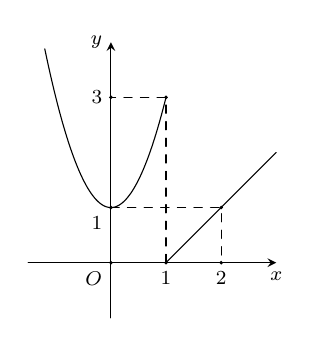
\begin{tikzpicture}[line join = round,line cap = round,>=stealth,font=\footnotesize,scale=0.7]
		\draw[->] (-1.5,0)--(3,0) node[below]{$x$}; 
		 \draw[->] (0,-1)--(0,4) node[left]{$y$};
		\fill (0,0) circle (1pt)  node[below left]{$O$};
		\draw (1,0)--(3,2); 
		\draw[samples=100,domain=-1.2:1,smooth] plot (\x,{2*(\x)^2+1}); 
		\fill (1,0) node[below] {$1$} circle  (1pt);
		\fill (0,1) node[below left] {$1$} circle (1pt); 
		\fill (0,3) node[left] {$3$}  circle (1pt);
		\fill (2,0) node[below] {$2$}  circle (1pt);
		 \fill (1,3) circle (1pt);
		\fill  (2,1) circle (1pt);
		 \draw[dashed] (1,0)--(1,3)--(0,3)
			 (0,1)--(2,1)--(2,0);
	\end{tikzpicture}
		} 
	 \loigiai{
		Dựa vào đồ  thị, ta thấy hàm số $y=f(x)$ liên tục trên các khoảng $(-\infty;1)$ và $(1;+\infty)$.
	} 
\end{ex}

% từ: cau-hoi/lop11/1D3_Gioi_han_Ham_so_lien_tuc/1D3-3-4_Ham_so_lien_tuc_tren_khoang_doan.tex
\begin{ex}%[1D3H3-4]%[ma:f3015208]
	Tìm các khoảng liên tục của hàm  số
	\begin{enumEX}[]{4}
		 \item $y=x^3+3x^2+x$;
		 \item $y=\dfrac{x-1}{x+1}$;
		\item  $y=\dfrac{x+1}{x^2+x-2}$;
		\item $y=\tan x+\cos  x$.
	\end{enumEX}
	\loigiai{ 
		\begin{enumerate}
			 \item Hàm số $y=x^3+3x^2+x$ có tập xác định $\mathscr{D}=\mathbb{R}$ nên hàm số liên tục trên $\mathbb{R}$.
			\item Hàm số $y=\dfrac{x-1}{x+1}$ có tập xác định $\mathscr{D}=\mathbb{R}\backslash \{1\}$ nên hàm số liên  tục trên $(-\infty;1)$, $(1;+\infty)$.
			\item Hàm số $y=\dfrac{x+1}{x^2+x-2}$ có tập  xác định $\mathscr{D}=\mathbb{R}\backslash \{1;-2\}$ nên hàm số liên tục trên các khoảng $(-\infty;-2)$, $(-2;1)$, $(1;+\infty)$.
			\item Hàm số $y=\tan  x+\cos x$ có tập xác định $\mathscr{D}=\mathbb{R}\backslash \left\{\dfrac{\pi}{2}+k\pi, k\in \mathbb{Z} \right\}$ nên hàm số liên tục trên các khoảng $\left(-\dfrac{\pi}{2}+k2\pi;\dfrac{\pi}{2}+k2\pi \right)$.
		\end{enumerate}
	 }
\end{ex}

% từ: cau-hoi/lop11/1D3_Gioi_han_Ham_so_lien_tuc/1D3-3-5_Bai_toan_phuong_trinh_co_nghiem.tex
\begin{ex}%[1D3H3-5]%[ma:25e539df]
	Cho phương trình $4x^4+2x^2-x-3=0$ $(1)$.  Mệnh đề nào dưới đây đúng?
	\choice 
		{Phương trình $(1)$ vô nghiệm  trên khoảng $\left(-1; 1\right)$}
		{Phương trình $(1)$ có đúng một nghiệm trên  khoảng $\left(-1; 1\right)$}
		{Phương trình $(1)$ có  đúng hai nghiệm trên khoảng $\left(-1; 1\right)$}
		{\True Phương trình $(1)$ có ít  nhất hai nghiệm trên khoảng $\left(-1; 1\right)$}
	\loigiai{ 
		Xét $f(x)=4x^4+2x^2-x-3=0$ trên khoảng $\left[-1; 1\right]$. 
		Ta có $f(x)$ liên tục trên đoạn $\left[-1; 1\right]$, và $\heva{f\left(-1\right)&=4\\ f(0)&=-3\\ f(1)&=2}\Rightarrow \heva{f\left(-1\right)\cdot f(0) &< 0\\ f(1)\cdot f(0)  &< 0.}$
		Do đó $f(x)=0$  có ít nhất hai nghiệm trên khoảng $\left(-1; 1\right)$.
	 }
\end{ex}

% từ: cau-hoi/lop11/1D3_Gioi_han_Ham_so_lien_tuc/1D3-3-5_Bai_toan_phuong_trinh_co_nghiem.tex
\begin{ex}%[1D3H3-5]%[ma:bf93cf0a]
	Cho phương trình $2x^4-5x^2+x+1=0(1)$. Chọn khẳng định  đúng trong các khẳng định sau
	 \choice
		{Phương  trình $(1)$ có đúng một nghiệm trên khoảng $\left(-2; 1\right)$}
		{Phương trình $(1)$ vô nghiệm} 
		{\True Phương trình $(1)$ có ít  nhất hai nghiệm trên khoảng $\left(0; 2\right)$}
		{Phương  trình $(1)$ vô nghiệm trên khoảng $\left(-1; 1\right)$}
	 \loigiai{
		Ta có: $\heva{&  f(-1)=-3 \\& f(0)=1 \\ &{f(1)=-1} \\& f(2)=15.}$
	 }
\end{ex}

% từ: cau-hoi/lop11/1D3_Gioi_han_Ham_so_lien_tuc/1D3-3-5_Bai_toan_phuong_trinh_co_nghiem.tex
\begin{ex}%[1D3H3-5]%[ma:94fd1d61]
	Tìm tất cả các giá  trị của tham số $m$ để phương trình $(m^2-3m+2)x^3-3x+1=0$ có nghiệm.
	\loigiai{ 
		Đặt $\left\{\begin{aligned}
		& f(x)=(m^2-3m+2)x^3-3x+1 \\ 
		& A=m^2-3m+2  \\
	\end{aligned} \right.$ \\
	Xét $A=m^2-3m+2=0 \Leftrightarrow $  $m=1$ hoặc $m=2$.\\
	Khi đó phương  trình trở thành $-3x+1=0 \Leftrightarrow x=\dfrac{1}{3}$. \\
	Xét $A=m^2-3m+2\ne  0 \Leftrightarrow $ $m\ne 1$ và $m\ne 2$.\\
	Khi đó: 
	\begin{itemize}
		\item Xét hàm số  $f(x)=(m^2-3m+2)x^3-3x+1$ đây là hàm đa thức, xác định trên $\mathbb{R}$ nên liên tục trên $\mathbb{R}$.
		 \item Mặt khác, ta có:
		\begin{itemize}[]
			\item [\bf TH 1.]  $A>0 \Rightarrow m\in (-\infty;1)\cup (2;+\infty)$. \\
			$\lim\limits_{x\to+\infty}f(x) =\lim\limits_{x\to+\infty}\left[Ax^3-3x+1 \right] =+\infty$ nên  tồn tại $x_1\in \mathbb{R}$ sao cho $f(x_1)>0$.\\
			$\lim\limits_{x\to-\infty}f(x) =\lim\limits_{x\to-\infty}\left[Ax^3-3x+1 \right] =-\infty$ nên tồn tại $x_2\in \mathbb{R}$ sao cho $f(x_2) <  0$.\\
			Áp dụng hệ  quả của định lí về giá trị trung gian, suy ra tồn tại $t\in (x_2;x_1)$ sao cho $f(t)=0$.\\
			\item [\bf  TH 2.] $A< 0\Rightarrow m\in (1;2)$. \\
			$\lim\limits_{x\to+\infty}f(x)  =\lim\limits_{x\to+\infty}\left[Ax^3-3x+1 \right]=-\infty$ nên tồn tại $x_1\in \mathbb{R}$ sao cho $f(x_1)<0$.\\
			$\lim\limits_{x\to-\infty}f(x) =\lim\limits_{x\to-\infty}\left[Ax^3-3x+1 \right]=+\infty$ nên tồn tại $x_2\in \mathbb{R}$  sao cho $f(x_2) > 0$.\\
			Áp dụng hệ quả của định lí về giá trị trung gian, suy ra tồn  tại $t\in (x_2;x_1)$ sao cho $f(t)=0$.
		\end{itemize}
		Vậy  phương trình đã cho có nghiệm với mọi $m\in \mathbb{R}$.
	\end{itemize}
	 }
\end{ex}

% từ: cau-hoi/lop11/1D5_Cac_so_dac_trung_do_xu_the_trung_tam_cho/1D5-1-1_Cau_hoi_ly_thuyet.tex
\begin{bt}%[1D5B1-1]%[ma:8c565526]
	Tính đạo hàm bằng định nghĩa của hàm số $y=f(x)=x^3-3x^2$ tại  điểm $x_0=1$.
	\loigiai{Ta có $\displaystyle \lim \limits_{x \to 1}\dfrac{x^3-3x^2-(-2)}{x-1}=\displaystyle \lim \limits_{x \to 1}\dfrac{(x^2-2x-2)(x-1)}{x-1}=\displaystyle \lim \limits_{x \to 1}(x^2-2x-2)=-3$. 
	} 
\end{bt}

% từ: cau-hoi/lop11/1D6_Ham_so_mu_va_ham_so_logarit/1D6-1-4_So_sanh_cac_luy_thua.tex
\begin{bt}%[1D6H1-4]%[ma:b503a9f7]
% nguon: Archive/2024/TOAN_11_XE/TOAN_11_XE/data4/11C6/KNTT-6.3.tex #1011
%[Tex hóa SGK CD-CT,T7/22, TVN-019]
	So sánh các cặp số sau:
	\begin{enumEX}{2}
		\item $1{,}3^{0{,}7}$ và $1{,}3^{0{,}6}$.
		\item $0{,}75^{-2{,}3}$ và $0{,}75^{-2{,}4}$.
	\end{enumEX}
	\loigiai{\begin{enumerate}
			\item Do $1{,}3>1$ nên hàm số $y=1{,}3^x$ đồng biến trên $\mathbb{R}$. Mà $0{,}7>0{,}6$ nên $1{,}3^{0{,}7}>1{,}3^{0{,}6}$.
			\item Do $0{,}75<1$ nên hàm số $y=0{,}75^x$ nghịch biến trên $\mathbb{R}$. Mà $-2{,}3>-2{,}4$ nên $0{,}75^{-2{,}3}<0{,}75^{-2{,}4}$.
	\end{enumerate}}
\end{bt}

% từ: cau-hoi/lop11/1D6_Ham_so_mu_va_ham_so_logarit/1D6-3-3_Su_bien_thien_va_do_thi_cua_ham_so_mu_logarit.tex
\begin{ex}%[1D6N3-3]%[ma:4dfbeef1]
	 \immini{
	Đường cong hình  bên là đồ thị của hàm số nào dưới đây?
	 \choice
		 {$y=2^x$}
		 {$y=\log_2x$}
		 {\True $y=\log_{\tfrac{1}{2}}x$}
		{$y=\left(\dfrac{1}{2}\right)^x$} 
		}{ 
		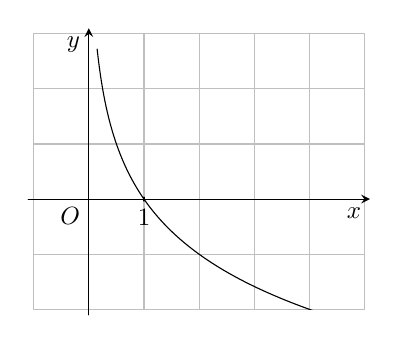
\begin{tikzpicture}[line join=round,line cap=round,>=stealth,scale=0.7]
				\draw[gray!50,xstep = 1,ystep = 1]  (-1,-2) grid (5,3);
				\draw[->]  (-1.1,0)--(5.1,0) node[below left] {$x$};
				\draw[->] (0,-2.1)--(0,3.1) node[below left] {$y$}; 
				\draw  (0,0) node [below left] {$O$};
				\foreach \x/\nx in {1/1} 
				\draw[thin]  (\x,1pt)--(\x,-1pt) node [below] {$\nx$};
				\begin{scope}
					 \clip (-1,-2) rectangle (5,3);
					 \draw[samples=200,domain=0.15:5,smooth,variable=\x] plot (\x,{ln((\x))/ln(0.5)});
				\end{scope}
			\end{tikzpicture}
		 }
	\loigiai{ 
		Hàm số xác định trên  $(0;+\infty)$.\\
		Hàm số nghịch biến trên  khoảng $(0;+\infty)$ nên cơ số $a\in (0;1)$.\\
		 Vậy hàm số $y=\log_{\tfrac{1}{2}}x$ có đồ thị như hình vẽ.
	 }
\end{ex}

% từ: cau-hoi/lop11/1D6_Ham_so_mu_va_ham_so_logarit/1D6-3-3_Su_bien_thien_va_do_thi_cua_ham_so_mu_logarit.tex
\begin{ex}%[1D6H3-3]%[ma:6c0c0987]
	\immini{Đường cong trong hình bên là của đồ thị  hàm số nào sau đây?
	\choice 
		{$y=\log_2  x$}
		 {\True $y=(0{,}8)^x$}
		 {$y=\log_{0{,}4} x$}
		{$y=\left(\sqrt{2}\right)^x$}}{\begin{tikzpicture}[line join = round,line cap = round,>=stealth,font=\footnotesize,scale =0.8]
		 \def\a{0.8}
		\def\f (#1){(\a)^(#1)} 
		 \def\xmin{-5}
		 \def\xmax{5}
		\def\ymin{-1} 
		 \def\ymax{4}
		\draw[->]  (\xmin,0)--(\xmax,0) node[below] {\footnotesize $x$};
		\draw[->] (0,\ymin)--(0,\ymax) node[right] {\footnotesize  $y$};
		\draw (0,0)  node [below left] {\footnotesize $O$};
		\draw[thick,smooth,samples=200] plot[domain=\xmin:\xmax]  (\x,{\f (\x)});
		 \path
			(0,1) node[below left]{$1$}; 
		\fill (0,1) circle (1pt); 
	\end{tikzpicture}
		} 
	\loigiai{Dựa vào đồ thị, ta có  hàm số có tập xác định $\mathbb{R}$ và hàm số nghịch biến suy ra $y=(0{,}8)^x$.}
\end{ex}

% từ: cau-hoi/lop11/1D6_Ham_so_mu_va_ham_so_logarit/1D6-3-3_Su_bien_thien_va_do_thi_cua_ham_so_mu_logarit.tex
\begin{ex}%[1D6H3-3]%[ma:b4afd773]
	 \immini{Cho hàm số $y=\log_a x$ ($a>0, a\neq 1$) có đồ thị như hình vẽ. Giá trị của $a$ bằng
	\choice 
		{$a=2$} 
		{\True  $a=\dfrac{1}{2}$}
		 {$a=\dfrac{1}{\sqrt{2}}$}
		{$a=\sqrt{2}$}}{\begin{tikzpicture}[line join = round,line cap = round,>=stealth,font=\footnotesize,scale =1]
		\def\a{0.5} 
		\def\f (#1){ln (#1)/ln (\a)} 
		 \def\xmin{-1}
		\def\xmax{4} 
		\def\ymin{-2.75} 
		\def\ymax{3} 
		 \def\n{0.15}
		\draw[->] (\xmin,0)--(\xmax,0) node[below] {\footnotesize $x$}; 
		\draw[->] (0,\ymin)--(0,\ymax) node[right] {\footnotesize $y$}; 
		\draw (0,0) node [below left]  {\footnotesize $O$};
		\draw[thick,smooth,samples=200]  plot[domain=
		\n:\xmax] (\x,{\f  (\x)});
		\draw[dashed]  (2,0)--(2,-1)--(0,-1);
		\path (1,0)  node[below]{$1$}
			 (2,0) node[above]{$2$}
			 (0,-1) node[left]{$-1$};
		 \fill (1,0) circle (1pt)
			(2,-1)  circle (1pt);
	\end{tikzpicture}
		 }
	\loigiai{Đồ thị hàm số $y=\log_a x$ đi qua điểm $(2;-1)$ nên $\log_a 2 =  -1$.\\
	Khi đó $a^{-1}=2\Leftrightarrow \dfrac{1}{a}=2 \Leftrightarrow a=\dfrac{1}{2}$.} 
\end{ex}

% từ: cau-hoi/lop11/1D6_Ham_so_mu_va_ham_so_logarit/1D6-3-3_Su_bien_thien_va_do_thi_cua_ham_so_mu_logarit.tex
\begin{ex}%[1D6H3-3]%[ma:4c74f9fa]
	Cho ba hàm  số $y=2^x$, $y=x$, $y=f(x)$ có đồ thị như hình bên, mệnh đề nào sau đây đúng?
	\begin{center}
		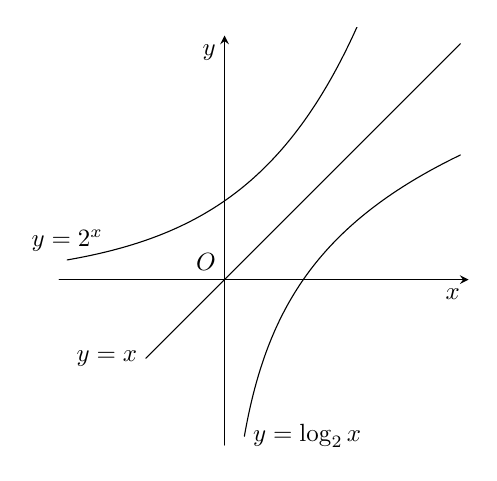
\begin{tikzpicture}[line join=round,line cap=round,>=stealth]
				\tikzset{every  node/.style={scale=0.9}}
				\draw[->] (-2.1,0)--(3.1,0) node[below left]  {$x$};
				\draw[->] (0,-2.1)--(0,3.1) node[below  left] {$y$};
				\draw (0,0)  node [above left] {$O$};
				\begin{scope}
					\clip  (-2.5,-2.2) rectangle (3,3.2);
					\draw[samples=200,domain=3:-2,smooth,variable=\x] plot  (\x,{2^(\x)}) node[above]{$y=2^x$};
					\draw[samples=200,domain=3:-1,smooth,variable=\x] plot  (\x,{1*(\x)}) node[left]{$y=x$};
					\draw[samples=200,domain=3:0.25,smooth,variable=\x] plot  (\x,{ln ((\x))/ln (2)}) node[right]{$y=\log_2x$};
				\end{scope}
			\end{tikzpicture}
	\end{center}
	 \choice
		 {$y=f(x)=\log_{\tfrac{1}{2}}x$}
		 {$y=f(x)=\ln x$}
		 {\True $y=f(x)=\log_2x$}
		 {$y=f(x)=\log x$}
	 \loigiai{
		Đồ thị hàm số $y=2^x$ và đồ thị hàm số $y=\log_2x$ đối xứng  nhau qua đường thẳng $y=x$.
	} 
\end{ex}

% từ: cau-hoi/lop11/1D6_Ham_so_mu_va_ham_so_logarit/1D6-3-3_Su_bien_thien_va_do_thi_cua_ham_so_mu_logarit.tex
\begin{ex}%[1D6H3-3]%[ma:bc497aa0]
	\immini{Đồ thị sau là đồ thị của hàm  số nào?
	 \choice
		 {$y=\log_2 x+1$}
		{$y=\log_2(x+1)  $}
		 {$y=\log_3 x$}
		{\True $y=\log_3(x+1) $}}{\begin{tikzpicture}[line join = round,line cap = round,>=stealth,font=\footnotesize,scale =1]
		 \def\a{3}
		\def\f (#1){ln (#1+1)/ln (\a)} 
		\def\xmin{-2} 
		\def\xmax{4} 
		 \def\ymin{-2.1}
		 \def\ymax{2}
		\def\n{-0.9} 
		\draw[->]  (\xmin,0)--(\xmax,0) node[below] {\footnotesize $x$};
		\draw[->] (0,\ymin)--(0,\ymax)  node[right] {\footnotesize $y$};
		\draw (0,0) node [below right] {\footnotesize $O$}; 
		\draw[thick,smooth,samples=200]  plot[domain=
		 \n:\xmax] (\x,{\f (\x)});
		 \draw[dashed] (2,0)--(2,1)--(0,1)
			(-1,\ymin)--(-1,\ymax); 
		\path (-1,0)  node[below left]{$-1$}
			 (2,0) node[below]{$2$}
			 (0,1) node[left]{$1$};
		\fill (1,2)  circle (1pt);
	\end{tikzpicture}
		} 
	 \loigiai{Dựa vào đồ thị, ta thấy\\
		Hàm số xác định trên  khoảng $(-1;+\infty)$ $\Rightarrow$ loại $y==\log_2 x+1$ và $y=\log_3 x$.\\
	Đồ thị hàm số đi qua điểm $(2;1)$.\\Vậy đồ thị đã cho  là hàm số $y=\log_3 (x+1)$.}
\end{ex}

% từ: cau-hoi/lop11/1D6_Ham_so_mu_va_ham_so_logarit/1D6-3-3_Su_bien_thien_va_do_thi_cua_ham_so_mu_logarit.tex
\begin{ex}%[1D6H3-3]%[ma:782fdd2c]
	Cho các đồ thị hàm số $y=a^x$, $y=\log_bx$,  $y=x^c$ ở hình vẽ sau đây.
	\begin{center}
		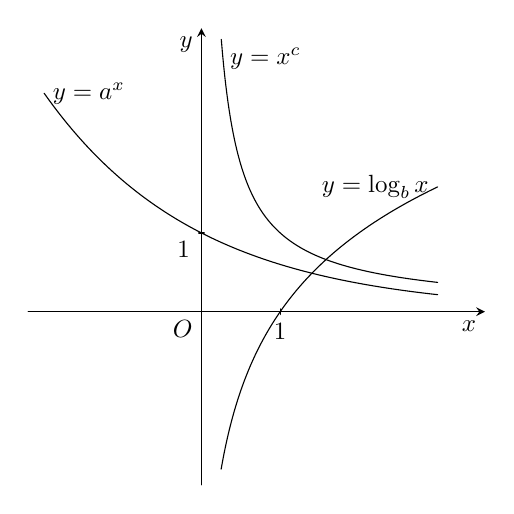
\begin{tikzpicture}[line join=round,line cap=round,>=stealth]
				\tikzset{every node/.style={scale=0.9}} 
				\draw[->] (-2.2,0)--(3.6,0) node[below  left] {$x$};
				\draw[->]  (0,-2.2)--(0,3.6) node[below left] {$y$};
				\draw (0,0) node [below left] {$O$}; 
				\foreach \x/\nx  in {1/1}
				\draw[thin] (\x,1pt)--(\x,-1pt) node  [below] {$\nx$};
				\foreach  \y/\ny in {1/1}
				\draw[thin] (1pt,\y)--(-1pt,\y) node  [below left] {$\ny$};
				\begin{scope}
					 \clip (-2.2,-2.2) rectangle (3.5,3.5);
					\draw[samples=200,domain=3:-2,smooth,variable=\x] plot  (\x,{0.6^(\x)}) node[right]{$y=a^x$};
					\draw[samples=200,domain=3:0.25,smooth,variable=\x] plot (\x,{(\x)^(-0.9)}) node[below  right]{$y=x^c$};
					\draw[samples=200,domain=0.25:3,smooth,variable=\x] plot (\x,{ln ((\x))/ln (2)})  node[left] {$y=\log_bx$};
				\end{scope}
			\end{tikzpicture}
	\end{center}
	Khẳng định nào sau  đây đúng?
	 \choice
		 {$0<c<1<a<b$}
		{\True  $c<0<a<1<b$}
		{$c<0<a<b<1$} 
		{$0<c<a<b<1$} 
	 \loigiai{
		Ta thấy đồ thị $y=x^c$ đi xuống nên  $c<0$, đồ thị $y=a^x$ đi xuống nên $0<a<1$, đồ thị $y=\log_bx$ đi lên nên $b>1$.
	 }
\end{ex}

% từ: cau-hoi/lop11/1D6_Ham_so_mu_va_ham_so_logarit/1D6-3-3_Su_bien_thien_va_do_thi_cua_ham_so_mu_logarit.tex
\begin{ex}%[1D6H3-3]%[ma:d7e3c34b]
	\immini{Trong hình vẽ bên có đồ thị của các hàm số $y=a^x$, $y=b^x$, $y=\log_c x$. Mệnh đề  nào sau đây đúng?
	 \choice
		{$a < b < c$} 
		{$a <  b=c$}
		{$b <  c < a$}
		{\True $a < c < b$}}{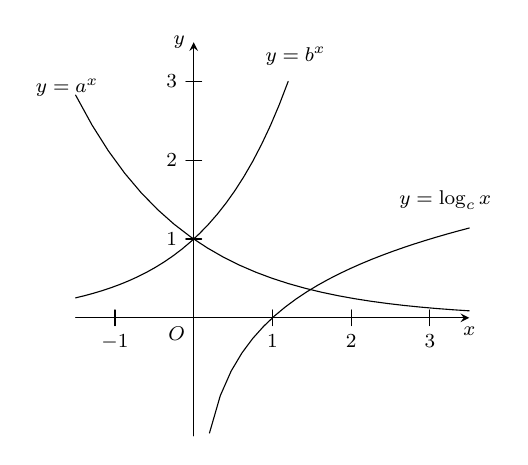
\begin{tikzpicture}[line join = round,line cap = round,>=stealth,font=\footnotesize,scale =1]
		 \draw[->] (-1.5,0) -- (3.5,0) node[below] {$x$};
		\draw[->] (0,-1.5) -- (0,3.5) node[left]  {$y$};
		\node at (0,0) [below left]{$O$}; 
		\foreach \x in {-1,1,2,3} 
		\draw  (\x,0.1) -- (\x,-0.1) node[below] {$\x$};
		\foreach \y in {1,2,3} 
		\draw (0.1,\y)  -- (-0.1,\y) node[left] {$\y$};
		 \draw[domain=-1.5:3.5] plot (\x,{(0.5)^\x});
		\node[above left] at (-1.1,2.7)  {$y = a^x$};
		 \draw[domain=-1.5:1.2] plot (\x,{(2.5)^\x});
		\node[above right] at (0.8,3.1) {$y = b^x$}; 
		\draw[domain=0.2:3.5] plot (\x,{ln (\x)/ln  (3)});
		\node[right]  at (2.5,1.5) {$y = \log_c x$};
	\end{tikzpicture}
		} 
	\loigiai{- Hàm số  $y=a^x$ nghịch biến trên $\mathbb{R}$ nên $0 < a < 1$.\\
		- Các hàm số $y=b^x$, $y=\log_c x$ đồng biến biến trên tập xác định của nó  nên $b$, $c > 1$.\\ Suy ra $0 < a < b, c < 1$.\\
		 - Xét đồ thị hàm số $y=\log_c x$, ta có $\log_c 2 > 1 \Leftrightarrow c < 2$.\\
	- Xét đồ thị hàm số $y=b^x$, ta có $b^1 >  2 \Leftrightarrow b > 2$. Do đó $0 < a < c < b$.}
\end{ex}

% từ: cau-hoi/lop11/1D6_Ham_so_mu_va_ham_so_logarit/1D6-3-3_Su_bien_thien_va_do_thi_cua_ham_so_mu_logarit.tex
\begin{ex}%[1D6H3-3]%[ma:1ea4c080]
	Tìm $a$ để đồ thị hàm số $y=\log_ax$, $(0<a\ne 1)$ có đồ thị  là hình bên.
	\begin{center}
		\begin{tikzpicture}[line join=round,line cap=round,>=stealth]
				\tikzset{every  node/.style={scale=0.9}}
				 \draw[->] (-1.1,0)--(4.1,0) node[below left] {$x$};
				\draw[->] (0,-1.1)--(0,4.1)  node[below left] {$y$};
				\draw (0,0) node [below left]  {$O$};
				 \foreach \x/\nx in {1/1,2/2}
				 \draw[thin] (\x,1pt)--(\x,-1pt) node [below] {$\nx$};
				\foreach  \y/\ny in {2/2}
				\draw[thin] (1pt,\y)--(-1pt,\y) node [left]  {$\ny$};
				 \draw[dashed,thin](2,0)--(2,2)--(0,2);
				\begin{scope}
					\clip (-1,-1) rectangle (4,4.5); 
					\draw[samples=200,domain=0.25:4,smooth,variable=\x]  plot (\x,{ln ((\x))/ln (sqrt (2))}) node[left]{$y=\log_ax$};
				\end{scope}
			\end{tikzpicture}
	\end{center}
	 \choice
		{\True $a=\sqrt{2}$} 
		{$a=\dfrac{1}{\sqrt{2}}$} 
		 {$a=\dfrac{1}{2}$}
		{$a=2$} 
	\loigiai{ 
		Do đồ thị hàm  số đi qua điểm $(2;2)$ nên $2=\log_a2\Leftrightarrow a=\sqrt 2$.
	 }
\end{ex}

% từ: cau-hoi/lop11/1D6_Ham_so_mu_va_ham_so_logarit/1D6-3-3_Su_bien_thien_va_do_thi_cua_ham_so_mu_logarit.tex
\begin{ex}%[1D6H3-3]%[ma:294ac1b8]
	\immini{Hình bên là đồ  thị của hàm số nào trong các hàm số sau đây?
	 \choice
		{\True $y=(0{,}4)^x$} 
		{$y=(\sqrt{2})^x$} 
		{$y=\log_2  x$}
		{$y=\log_{0{,}4} x$}}{\begin{tikzpicture}[line join = round,line cap = round,>=stealth,font=\footnotesize,scale =1]
		 \def\a{0.4}
		\def\f  (#1){(\a)^(#1)}
		\def\xmin{-3} 
		\def\xmax{3} 
		 \def\ymin{-1}
		\def\ymax{4} 
		\draw[->] (\xmin,0)--(\xmax,0) node[below] {\footnotesize $x$}; 
		\draw[->] (0,\ymin)--(0,\ymax)  node[right] {\footnotesize $y$};
		\draw  (0,0) node [below left] {\footnotesize $O$};
		\draw[thick,smooth,samples=200]  plot[domain=-1.5:\xmax] (\x,{\f (\x)});
		\path 
			(0,1) node[above right]{$1$}; 
		 \fill
			(0,1) circle  (1pt);
	\end{tikzpicture}
		} 
	 \loigiai{Hình bên là đồ thị của hàm mũ có cơ số $a$ thỏa $0 < a < 1$.}
\end{ex}

% từ: cau-hoi/lop11/1D6_Ham_so_mu_va_ham_so_logarit/1D6-3-3_Su_bien_thien_va_do_thi_cua_ham_so_mu_logarit.tex
\begin{ex}%[1D6H3-3]%[ma:4a9a928d]
	Trong hình vẽ bên có đồ thị các hàm số  $y=a^x$, $y=b^x$, $y=\log_cx$. Hãy chọn mệnh đề đúng trong các mệnh đề sau đây?
	\begin{center}
		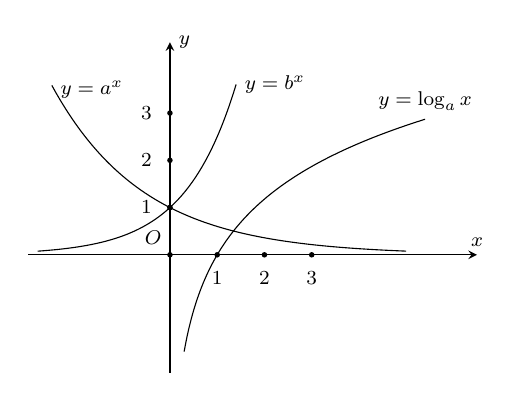
\begin{tikzpicture}[scale=1,>=stealth,font=\footnotesize,line join=round,line cap=roundm,x=0.6cm,y=0.6cm]
				\def \xmin{-3}; 
				\def  \xmax{6.5};
				\def \ymin{-2.5}; 
				\def \ymax{4.5}; 
				\draw[->] (\xmin,0) --  (\xmax,0) node[above] {$x$};
				\draw[->] (0.,\ymin) -- (0.,\ymax)  node[right] {$y$};
				\draw[smooth,samples=100,domain=-2.5:5] plot (\x,{(0.6^(\x))}); 
				\draw[smooth,samples=100,domain=-2.8:1.4] plot (\x,{(2.5^(\x))})  node[right]{$y=b^x$};
				\draw[smooth,samples=100,domain=0.3:5.4] plot (\x,{(ln(\x))/(ln(1.8))})  node[above]{$y=\log_ax$};
				\draw  (-2.5,3.5) node[right]{$y=a^x$};
				 \foreach \x/\y/\l/\g in {0/0/O/135,0/1/1/180,1/0/1/-90,0/1//0,0/2/2/180,0/3/3/180,2/0/2/-90,3/0/3/-90}{\fill[black] (\x,\y) circle (1pt)+(\g:0.5) node{$\l$};}
			\end{tikzpicture}
	\end{center}
	\choice 
		{\True $a < c  < b$}
		{$c  < a < b$}
		{$a < b=c$} 
		{$b <  c < a$}
	\loigiai{ 
		Hàm số $y=a^x$ nghịch biến  trên $\mathbb{R}$ nên ta có $0 < a < 1$.\\
		Các hàm số $y=b^x$, $y=\log_cx$ đồng  biến biến trên tập xác định của nó nên ta có $\heva{&b > 1\\&c > 1.}$\\
		Xét đồ thị hàm số $y=\log_cx$, ta có $\log_c2 > 1\Leftrightarrow c  < 2$.\\
		Xét đồ thị hàm số $y=b^x$, ta có $b^1> 2\Leftrightarrow b > 2$.\\ 
		Do đó $0 <  a < c < b$.
	} 
\end{ex}

% từ: cau-hoi/lop11/1D6_Ham_so_mu_va_ham_so_logarit/1D6-3-3_Su_bien_thien_va_do_thi_cua_ham_so_mu_logarit.tex
\begin{ex}%[1D6H3-3]%[ma:0a59667f]
	\immini{Hàm số  nào sau đây có đồ thị như hình bên?
	 \choice
		 {$y=\log_3x$}
		 {$y=\log_2x+1$}
		{\True  $y=\log_2(x+1)$}
		{$y=\log_3(x+1)$} 
		}{\begin{tikzpicture}[scale=1,font=\footnotesize,line join=round,line cap=round,>=stealth,x=0.6cm,y=0.6cm,declare function = {f (\x) =ln((\x)+1)/ln(2);}]
		\def  \xmin{-1.5};
		 \def \xmax{3.7};
		\def \ymin{-1.5}; 
		 \def \ymax{2.7};
		\draw[->] (\xmin,0.) -- (\xmax,0.) node[anchor=north]  {$x$};
		 \draw[->] (0.,\ymin) -- (0.,\ymax) node[anchor=west] {$y$};
		\clip (\xmin+0.1,\ymin+0.1) rectangle (\xmax-0.1,\ymax-0.1); 
		\draw[smooth,samples=100,domain=-0.9:\xmax]  plot (\x,{f (\x)});
		\draw[dashed]  (1,0) node[below]{$1$} |- (0,1) node[left]{$1$};
		\foreach \x/\y/\l/\g in {0/0/O/135,1/1//0,1/0//0,0/1//0}{\fill[black] (\x,\y) circle  (1pt)+(\g:0.5) node{$\l$};}
	\end{tikzpicture}
		} 
	\loigiai{ 
		Đồ thị trong hình vẽ  đi qua điểm $(0;0)$ và $(1;1)$.\\
		Trong $4$ phương án  chỉ có hàm số $y=\log_2 (x+1)$ có đồ thị phù hợp.
	} 
\end{ex}

% từ: cau-hoi/lop11/1D6_Ham_so_mu_va_ham_so_logarit/1D6-3-3_Su_bien_thien_va_do_thi_cua_ham_so_mu_logarit.tex
\begin{ex}%[1D6H3-3]%[ma:45e7c50e]
	\immini 
	 {
	Đường  cong trong hình bên là đồ thị của hàm số nào sau đây?
	 \choice
		{$y=\log  _2(2 x)$}
		 {$y=\log _{\tfrac{1}{2}}x$}
		{$y=\log _{\sqrt{2}}x$} 
		{\True $y=\log _2  x$}
		 }
		 {
		\begin{tikzpicture}[>=stealth,scale=0.7]
				\def\xmax{3} \def\xmin{-1}  \def\ymax{2} \def\ymin{-3.5}
				\draw[->] (\xmin,0) -- (\xmax,0) node[below]{\footnotesize $x$}; 
				\draw[->] (0,\ymin) --  (0,\ymax) node[left] {\footnotesize $y$};
				\draw (0,0) node[below left]{\footnotesize $O$}; \fill (0,0)  circle (1pt);
				\foreach  \x in{}
				\draw[shift={(\x,0)}]  (0,-2pt)--(0,2pt) node[below]{\footnotesize $\x$};
				 \foreach \y in{1}
				\draw[shift={(0,\y)}] (-2pt,0)--(2pt,0) node[left]{\footnotesize $\y$}; 
				\foreach \y in{-1} 
				\draw[shift={(0,\y)}] (-2pt,0)--(2pt,0) node[left]{\footnotesize  $\y$};
				 \draw[smooth,domain=0.1:3]plot (\x,{ln(\x)/ln(2)}) node[above] {};
				\foreach \x/\y in{0.5/-1}{\fill (\x,\y) circle (1pt); \draw[dashed](\x,0)--(\x,\y)--(0,\y);} 
				\draw (0.5,0) node[above]{\footnotesize  $\dfrac{1}{2}$};
			\end{tikzpicture}
		} 
	\loigiai{ 
		Đồ thị hàm số $y=\log  _2 x$.
	} 
\end{ex}

% từ: cau-hoi/lop11/1D6_Ham_so_mu_va_ham_so_logarit/1D6-3-3_Su_bien_thien_va_do_thi_cua_ham_so_mu_logarit.tex
\begin{ex}%[1D6H3-3]%[ma:eb664fa8]
	 \immini
	 {
	Cho hai hàm số $y=a^x$ và $y=\log_b x$ có đồ thị như hình  vẽ. Mệnh đề nào sau đây là đúng.
	 \choice
		{\True $a>1; 0<b<1$} 
		{$0<a<1; 0<b<1$} 
		{$0<a<1;  b>1$}
		 {$a>1; b>1$}
		} 
		{ 
		\begin{tikzpicture}[>=stealth,scale=0.7,line join=round,line cap=round]
				\draw[->] (-2,0)--(4,0) node  [below]{$x$};
				\draw[->]  (0,-2)--(0,3) node [left]{$y$};
				\node at (0,0) [below right]{$O$}; 
				\clip (-3,-3)  rectangle (4,4);
				\fill[black](0,1) circle (1pt)  node[above left] {$1$}
					(1,0) circle (1pt) node [below] {$1$}; 
				\draw[smooth,samples=150,domain=-2:1.5] plot (\x,{2^(\x)}); 
				\draw[smooth,samples=150,domain=0.3:3] plot (\x,{-ln(\x)/ln(2)}); 
				\node at (2,2){$y=a^x$}; 
				\node  at (1.7,-0.6)[right]{$y=\log_{b}x$};
			\end{tikzpicture}
		 }
	 \loigiai{
		Quan sát  đồ thị ta thấy :\\
		Hàm số $y=a^x$  đồng biến nên $a>1$.\\
		Hàm  số $y=\log_b x$ nghịch biến nên $0<b<1$.
	} 
\end{ex}

% từ: cau-hoi/lop11/1D6_Ham_so_mu_va_ham_so_logarit/1D6-3-3_Su_bien_thien_va_do_thi_cua_ham_so_mu_logarit.tex
\begin{ex}%[1D6H3-3]%[ma:b5f8504c]
	Hàm  số nào sau đây có đồ thị như hình bên?
	\begin{center}
		\begin{tikzpicture}[scale=1,font=\footnotesize,line join=round,line cap=round,>=stealth,x=0.6cm,y=0.6cm,declare function = {f (\x) =ln((\x)+1)/ln(2);}]
				\def \xmin{-1.5}; 
				 \def \xmax{3.7};
				\def \ymin{-1.5}; 
				 \def \ymax{2.7};
				\draw[->]  (\xmin,0.) -- (\xmax,0.) node[anchor=north] {$x$};
				\draw[->] (0.,\ymin) -- (0.,\ymax)  node[anchor=west] {$y$};
				 \clip (\xmin+0.1,\ymin+0.1) rectangle (\xmax-0.1,\ymax-0.1);
				\draw[smooth,samples=100,domain=-0.9:\xmax]  plot (\x,{f (\x)});
				\draw  (-1,-1.4)--(-1,3.6);
				\draw[dashed]  (1,0) node[below]{$1$} |- (0,1) node[left]{$1$};
				\foreach \x/\y/\l/\g in {0/0/O/135,1/1//0,1/0//0,0/1//0}{\fill[black] (\x,\y)  circle (1pt)+(\g:0.5) node{$\l$};}
			\end{tikzpicture}
	\end{center}
	\choice 
		{$y=\log_3x$} 
		{$y=\log_2x+1$} 
		{\True $y=\log_2(x+1)$} 
		 {$y=\log_3(x+1)$}
	\loigiai{ 
		Đồ thị hàm số đi qua điểm $(0;0)$ nên loại phương án $y=\log_3x$ và $y=\log_2x+1$.\\ 
		Đồ thị hàm số đi qua  điểm $(1;1)$ nên loại phương án $y=\log_3(x+1)$.\\
		Vậy đáp án $y=\log_2\left(x+1\right)$  thỏa mãn.
	 }
\end{ex}

% từ: cau-hoi/lop11/1D6_Ham_so_mu_va_ham_so_logarit/1D6-3-3_Su_bien_thien_va_do_thi_cua_ham_so_mu_logarit.tex
\begin{ex}%[1D6H3-3]%[ma:00b74eab]
	\immini{ 
	Cho hàm số $y=\log_ax\left(a>0, a\neq 1\right)$ có đồ thị như hình vẽ. Giá trị của $a$  bằng
	\choice 
		 {$a=2$}
		{$a=\sqrt{2}$} 
		 {$a=\dfrac{1}{\sqrt{2}}$}
		{\True  $a=\dfrac{1}{2}$}
		}{ 
		\begin{tikzpicture}[scale=0.7,font=\footnotesize,line join=round,line cap=round,>=stealth]
				\def\xmax{5}  \def\ymin{-3} \def\ymax{3}
				 \draw[->] (-0.9,0)--(\xmax,0) node [below]{$x$};
				\draw[->] (0,\ymin)--(0,\ymax) node [left]{$y$}; 
				\node at (0,0)  [above left]{$O$};
				\clip  (-0.9,\ymin) rectangle (\xmax-0.1,\ymax-0.1);
				\draw[smooth,samples=300,domain=0.03:\xmax] plot  (\x,{ln(\x)/ln(0.5)});
				\draw[dashed]  (2,0) node[above]{$2$}--(2,-1)--(0,-1) node[left]{$-1$};
				\fill (1,0) circle (1.0pt)  node[below]{$1$}
					(2,0) circle  (1.0pt)
					(0,-1) circle  (1.0pt);
			\end{tikzpicture}
		} 
	 \loigiai{
		Đồ thị hàm số $y=\log_ax$ đi qua điểm $(2;-1)$ nên  $\log_a2=-1$.\\
	 Khi đó $a^{-1}=2\Leftrightarrow\dfrac{1}{a}=2\Leftrightarrow a=\dfrac{1}{2}$.}
\end{ex}

% từ: cau-hoi/lop11/1D6_Ham_so_mu_va_ham_so_logarit/1D6-3-3_Su_bien_thien_va_do_thi_cua_ham_so_mu_logarit.tex
\begin{ex}%[1D6V3-3]%[ma:c65a8dc1]
	\immini{Cho đồ thị hàm số $y=a^x$ và $y=\log_bx$ như  hình vẽ bên. Khẳng định nào sau đây đúng?
	\choice 
		{$0<a<\dfrac{1}{2}<b$} 
		{\True $0<a<1<b$} 
		{$0<b<1<a$} 
		{$0<a<1$, $0<b<\dfrac{1}{2}$}}{\begin{tikzpicture}[scale=1,font=\footnotesize,line join=round,line cap=round,>=stealth,x=0.6cm,y=0.6cm,declare function = {f (\x)=ln(\x)/ln(2); g (\x)=0.6^(\x);}]
		\def  \xmin{-2.5};
		\def  \xmax{3.7};
		 \def \ymin{-1.5};
		 \def \ymax{3.5};
		\draw[->] (\xmin,0.) -- (\xmax,0.) node[anchor=north] {$x$}; 
		\draw[->] (0.,\ymin) --  (0.,\ymax) node[anchor=west] {$y$};
		\clip (\xmin+0.1,\ymin+0.1) rectangle (\xmax-0.1,\ymax-0.1); 
		 \draw[smooth,samples=100,domain=0.1:\xmax] plot (\x,{f (\x)});
		\draw[smooth,samples=100,domain=\xmin:\xmax] plot (\x,{g (\x)}); 
		\foreach \x/\y/\l/\g in {0/0/O/225,0/1/1/180,1/0/1/-90}{\fill[black] (\x,\y) circle (1pt)+(\g:0.5)  node{$\l$};}
	\end{tikzpicture}
		 }
	\loigiai{ 
		Đồ thị hàm số $y=a^x$ đi qua $\left(0;1\right)$ nên từ hình vẽ suy ra hàm số $y=a^x$ là hàm  nghịch biến. Do đó $0<a<1$.\\
		Đồ thị hàm số $y=\log_bx$ đi qua $\left(1;0\right)$ nên từ hình vẽ suy ra hàm số  $y=\log_b x$ là hàm đồng biến. Do đó $b>1$.\\
		 Vậy $0<a<1<b$.
	 }
\end{ex}

% từ: cau-hoi/lop11/1D6_Ham_so_mu_va_ham_so_logarit/1D6-3-3_Su_bien_thien_va_do_thi_cua_ham_so_mu_logarit.tex
\begin{ex}%[1D6V3-3]%[ma:e26eb24f]
	\immini{Cho đồ thị hàm số $y=a^x$ và $y=\log_bx$ như hình vẽ bên. Trong các  khẳng định sau, đâu là khẳng định đúng?
	 \choice
		{$0<a<1,0<b<1$} 
		 {$a>1,b>1$}
		{\True  $0<b<1<a$}
		{$0<a<1<b$}}{\begin{tikzpicture}[scale=1,font=\footnotesize,line join=round,line cap=round,>=stealth,x=0.6cm,y=0.6cm,declare function = {f (\x)=ln(\x)/ln(0.5); g (\x)=1.8^(\x);}]
		 \def \xmin{-2.5};
		\def \xmax{3.7}; 
		\def \ymin{-1.5}; 
		 \def \ymax{3.5};
		\draw[->] (\xmin,0.) -- (\xmax,0.)  node[anchor=north] {$x$};
		\draw[->]  (0.,\ymin) -- (0.,\ymax) node[anchor=west] {$y$};
		\clip (\xmin+0.1,\ymin+0.1)  rectangle (\xmax-0.1,\ymax-0.1);
		\draw[smooth,samples=100,domain=0.1:\xmax] plot (\x,{f (\x)}); 
		\draw[smooth,samples=100,domain=\xmin:\xmax]  plot (\x,{g (\x)});
		 \foreach \x/\y/\l/\g in {0/0/O/225,0/1/1/180,1/0/1/-90}{\fill[black] (\x,\y) circle (1pt)+(\g:0.5) node{$\l$};}
	\end{tikzpicture}
		 }
	\loigiai{ 
		Đồ thị hàm số $y=a^x$ đi qua $\left(0;1\right)$ nên  từ hình vẽ suy ra hàm số $y=a^x$ là hàm đồng biến. Do đó $a>1$.\\
		Đồ  thị hàm số $y=\log_bx$ đi qua $\left(1;0\right)$ nên từ hình vẽ suy ra hàm số $y=\log_b x$ là hàm nghịch biến. Do đó $0<b<1$.\\
		Vậy $0<b<1<a$. 
	 }
\end{ex}

% từ: cau-hoi/lop11/1D6_Ham_so_mu_va_ham_so_logarit/1D6-3-3_Su_bien_thien_va_do_thi_cua_ham_so_mu_logarit.tex
\begin{ex}%[1D6H3-3]%[ma:994653ca]
	Cho hàm  số $ y=2^x$
	\choiceTF 
		{\True  Hàm số có tập xác định $ \mathscr{D}=\mathbb{R} $}
		{Hàm số nghịch biến trên khoảng $\left(-\infty;+\infty\right)$} 
		{\True Đồ thị hàm số đi qua điểm $ A\left(2;4\right)$} 
		{\True  Đồ thị hàm số có hình sau}
		\begin{center}
			\begin{tikzpicture}[line join = round,line cap = round,>=stealth,font=\footnotesize,scale =1]
					\draw[->,line width = 1pt]  (-3,0)--(0,0) node[below right]{$O$}--(4.5,0) node[below]{$x$};
					\draw[->,line width =  1pt] (0,-1)--(0,4.5) node[right]{$y$};
					 \foreach \x in {-2,-1,1,2} \draw[thin] (\x,2pt)--(\x,-2pt) node [below] {$\x$};
					\foreach \y in {2,4} \draw[thin] (2pt,\y)--(-2pt,\y) node  [left] {$\y$};
					\path (2.5,4) node  [below right]{$ y=2^x $};
					\clip (-3,-1) rectangle (3,4.5); 
					\draw[samples=300,domain=-3:4.5,smooth] plot (\x,{(2)^(\x)}); 
					\draw[dashed] (1,0)--(1,2)--(0,2) 
						(2,0)--(2,4)--(0,4); 
					\fill[black] (1,2) circle (1pt) 
						(2,4)  circle (1pt);
				\end{tikzpicture}
	\end{center}
	\loigiai{ 
		\begin{itemchoice}
			\itemch 
			Hàm số có tập xác định  $ \mathscr{D}=\mathbb{R} $.
			\itemch 
			Hàm  số đồng biến trên $\mathbb{R}$.
			\itemch 
			Ta thấy với $ x=2 $  thì $ y=2^x=4 $ nên đồ thị hàm số đi qua $ A(2;4) $.
			 \itemch
			Đồ thị chính  là đồ thị của hàm số $ y=2^x $.
		\end{itemchoice}
	 }
\end{ex}

% từ: cau-hoi/lop11/1D6_Ham_so_mu_va_ham_so_logarit/1D6-3-3_Su_bien_thien_va_do_thi_cua_ham_so_mu_logarit.tex
\begin{ex}%[1D6H3-3]%[ma:72c8e2f2]
	Cho hàm số $  y=\dfrac{1}{3^x}$.
	 \choiceTF
		{\True Hàm  số có tập xác định là $ \mathscr{D}=\mathbb{R} $}
		{Hàm số đồng biến trên $  (-\infty;+\infty)$}
		{Hàm số đi qua điểm $  A\left(-2;-9\right)$}
		{\True Hàm số có bảng biến  thiên như hình sau}
		\begin{center}
			\begin{tikzpicture}[line join = round,line cap = round,>=stealth,font=\footnotesize,scale =.8]
					\draw[->,line width = 1pt] (-3,0)--(0,0) node[below right]{$O$}--(2.5,0) node[below]{$x$}; 
					 \draw[->,line width = 1pt] (0,-1)--(0,9.5) node[right]{$y$};
					\foreach \x in {-2,-1,1,2} \draw[thin] (\x,2pt)--(\x,-2pt)  node [below] {$\x$};
					\foreach \y in  {3,9} \draw[thin] (2pt,\y)--(-2pt,\y) node [right] {$\y$};
					 \path (-2,9) node [below left]{$ y=\dfrac{1}{3^x} $};
					\clip (-3,-1)  rectangle (2.5,9.5);
					 \draw[samples=300,domain=-3:4.5,smooth] plot (\x,{(1/3)^(\x)});
					 \draw[dashed] (-2,0)--(-2,9)--(0,9)
						(-1,0)--(-1,3)--(0,3); 
					\fill[black] (-2,9)  circle (1pt)
						(-1,3)  circle (1pt);
				\end{tikzpicture}
	\end{center}
	\loigiai{ 
		\begin{itemchoice}
			 \itemch
			Hàm số có tập  xác định $ \mathscr{D}=\mathbb{R} $.
			\itemch 
			Hàm  số nghịch biến trên $\mathbb{R}$.
			\itemch 
			Ta thấy với $ x=-2 $ thì $ y=\dfrac{1}{3^{-2}}=9 $  nên đồ thị hàm số đi qua điểm $ (-2;9) $.
			\itemch 
			Đồ thị chính là đồ thị của hàm số  $ y=\left(\dfrac{1}{3}\right)^x $.
		\end{itemchoice}
	 }
\end{ex}

% từ: cau-hoi/lop11/1D6_Ham_so_mu_va_ham_so_logarit/1D6-3-3_Su_bien_thien_va_do_thi_cua_ham_so_mu_logarit.tex
\begin{ex}%[1D6H3-3]%[ma:633395b5]
	Cho số thực dương $a$ khác $1$. Biết rằng bất kỳ đường thẳng nào song song với trục $Ox$ mà cắt  các đường $y=4^x$, $y=a^x$, trục tung lần lượt tại $M$, $N$ và $A$ thì $AN=2AM$. Giá trị của $a$ bằng bao nhiêu?
	\begin{center}
		\begin{tikzpicture}[scale=1,>=stealth,font=\scriptsize,line join=round,line cap=round]
				\draw[->] (-3,0)--(3,0)  node[below] {$x$};
				\draw[->] (0,-1)--(0,3.5) node[left] {$y$}; 
				\fill  (0,0) circle (1pt) node[below left]{$O$};
				\clip (-3,-1) rectangle  (3,3.5);
				\draw[domain=-3:3,samples=200,smooth] plot (\x,{0.5^(\x)}); 
				\draw[domain=-3:3,samples=200,smooth]  plot (\x,{4^(\x)});
				\fill  ({ln (2.5)/ln (.5)},2.5) circle (1pt) node[left]{$N$}
					({ln (2.5)/ln (4)},2.5) circle  (1pt) node[right]{$M$}
					(0,2.5) circle (1pt) node[above left]{$A$}; 
				\draw ({ln (2.5)/ln (.5)},2.5)--({ln (2.5)/ln (4)},2.5); 
			\end{tikzpicture}
	\end{center}
	\shortans{0,5} 
	\loigiai{ 
		Dựa vào đồ thị hàm số ta thấy hàm số $y=a^x$ nghịch biến nên  $0<a<\dfrac{1}{2}$.\\
		Mọi đường thẳng $y=m$  ($m>0$) đều cắt các đường $y=4^x$, $y=a^x$, trục tung lần lượt tại $M(\log_4 m;m)$, $N(\log_a m;m)$ và $A(0;m)$, theo bài ra ta có
		\allowdisplaybreaks 
		\begin{eqnarray*}
			 &&AN=2AM\\
			&\Leftrightarrow& |\log_a m|=2|\log_4  m|\\
			 &\Leftrightarrow& |\log_a m|=|\log_2 m|\\
			&\Leftrightarrow& \hoac{&\log_a m=\log_2 m \\&\log_a m=-\log_2 m}\\ 
			&\Leftrightarrow&  \hoac{&a=2 \\&a=\dfrac{1}{2}.}
		\end{eqnarray*}
		Đối chiếu  với điều kiện, ta được $a=\dfrac{1}{2}=0{,}5$.
	 }
\end{ex}

% từ: cau-hoi/lop11/1D6_Ham_so_mu_va_ham_so_logarit/1D6-3-3_Su_bien_thien_va_do_thi_cua_ham_so_mu_logarit.tex
\begin{ex}%[1D6V3-3]%[ma:6188bbe0]
	\immini{Cho các hàm số $y=\log_a  x$ và $y=\log_b x$ có đồ thị như hình vẽ bên. Đường thẳng $x=5$ cắt trục hoành, đồ thị hàm số $y=\log_a x$ và $y=\log_b x$ lần lượt tại $A$, $B$ và $C$ . Biết rằng $CB=2AB$ và $a = mb^n$ với $m, n$ là các số nguyên dương. Tính $m^2 + n^2$.
	\shortans{10} 
	}{ 
	\begin{tikzpicture}[scale=0.8,font=\footnotesize,line join=round,line cap=round,>=stealth]
			\tikzset{label style/.style={font=\footnotesize}} 
			 \def \xmin{-1}
			\def \xmax{7} 
			\def  \ymin{-2}
			\def  \ymax{4.5}
			 \def \hamso{sin (\x r)}
			\draw[->] (\xmin,0)--(\xmax,0) node[below left] {$x$}; 
			\draw[->] (0,\ymin)--(0,\ymax)  node[below left] {$y$};
			\draw (0,0) node  [below left] {$O$};
			\foreach  \x in {5}
			 \draw[thin] (\x,1pt)--(\x,-1pt) node [below left] {$\x$};
			\begin{scope}
				 \clip (\xmin+0.01,\ymin+0.01) rectangle (\xmax-0.01,\ymax-0.01);
				\draw[samples=350,domain=0.01:\xmax-0.01,smooth,variable=\x] plot (\x,{ln (\x)/ln (2)})  node[above left]{$\log_b x$};
				\draw[samples=350,domain=0.01:\xmax-0.01,smooth,variable=\x] plot (\x,{ln (\x)/ln (8)}) node[above  left]{$\log_a x$};
				\draw[samples=350,domain=0.01:\xmax-0.01,smooth,variable=\x] plot  (\x,{ln (\x)/ln (2)}) node[above left]{$\log_b x$};
				\draw (5,-0.8)--(5,4)  node[above]{$x=5$};
				\draw (5.,0.) circle (1.0pt) node[below right]{$A$}; 
				\draw (5.,{ln (5)/ln (8)})  circle (1.0pt) node[below right]{$B$};
				\draw (5.,{ln (5)/ln (2)}) circle  (1.0pt) node[below right]{$C$};
			\end{scope}
		\end{tikzpicture}
	 }
	\loigiai{Ta  có $A(5; 0)$, $B\left(5;\log_a5\right)$, $C\left(5;\log_b5\right)$. \\
	 Do đó
	\begin{eqnarray*}
		&CB=2AB &\Leftrightarrow\log_b5-\log_a5=2\log_a5\\ 
		&&\Leftrightarrow\log_b5=3\log_a5 \\ 
		 &&\Leftrightarrow \log_5a=3\log_5b\\
		&&\Leftrightarrow a=b^3. 
	\end{eqnarray*}
	Vậy $m=1$, $n=3$ nên $m^2  + n^2 = 10$.
	 }
\end{ex}

% từ: cau-hoi/lop11/1D6_Ham_so_mu_va_ham_so_logarit/1D6-3-3_Su_bien_thien_va_do_thi_cua_ham_so_mu_logarit.tex
\begin{bt}%[1D6V3-3]%[ma:1f6c976e]
% nguon: Archive/SP-4Phan-Dot3/Data/CD_1_OTGK2_De03.tex #4262
%
	\immini
	{Cho các hàm số $y=\log_{a} x$ và $y=\log_{b} x$ có đồ thị như hình vẽ bên. Đường thẳng $x=5$ cắt trục hoành, đồ thị hàm số $y=\log_{a} x$ và $y=\log_{b} x$ lần lượt tại $A$, $B$ và $C$ . Biết rằng $CB=2AB$ và $a=mb^n$ với $m$, $n$ là các số nguyên dương. Tính $m^2+n^2$.}
	{\begin{tikzpicture}[scale=0.8, font=\footnotesize, line join=round, line cap=round, >=stealth]
			\tikzset{label style/.style={font=\footnotesize}}
			\def \xmin{-1}
			\def \xmax{7}
			\def \ymin{-2}
			\def \ymax{4.5}
			\def \hamso{sin(\x r)}
			\draw[->] (\xmin,0)--(\xmax,0) node[below left] {$x$};
			\draw[->] (0,\ymin)--(0,\ymax) node[below left] {$y$};
			\draw (0,0) node [below left] {$O$};
			\foreach \x in {5}
			\draw[thin] (\x,1pt)--(\x,-1pt) node [below left] {$\x$};
			\begin{scope}
				\clip (\xmin+0.01,\ymin+0.01) rectangle (\xmax-0.01,\ymax-0.01);
				\draw[samples=350,domain=0.01:\xmax-0.01,smooth,variable=\x] plot (\x,{ln(\x)/ln(2)}) node[above left]{$\log_{b} x$};
				\draw[samples=350,domain=0.01:\xmax-0.01,smooth,variable=\x] plot (\x,{ln(\x)/ln(8)}) node[above left]{$\log_{a} x$};
				\draw[samples=350,domain=0.01:\xmax-0.01,smooth,variable=\x] plot (\x,{ln(\x)/ln(2)}) node[above left]{$\log_{b} x$};
				\draw(5,-0.8)--(5,4) node[above]{$x=5$};
				\draw(5.,0.) circle (1.0pt) node[below right]{$A$};
				\draw(5.,{ln(5)/ln(8)}) circle (1.0pt) node[below right]{$B$};
				\draw(5.,{ln(5)/ln(2)}) circle (1.0pt) node[below right]{$C$};
			\end{scope}
	\end{tikzpicture}}
	\loigiai{
		Ta có $A(5; 0)$, $B\left(5;\log_{a}5\right)$, $C\left(5;\log_{b}5\right)$.\\
		Do đó	
		\begin{eqnarray*}
			&CB=2AB &\Leftrightarrow \log_{b}5-\log_{a}5=2\log_{a}5\\
			&&\Leftrightarrow \log_{b}5=3\log_{a}5\\
			&&\Leftrightarrow \log_{5}a=3\log_{5}b\\
			&&\Leftrightarrow a=b^3.
		\end{eqnarray*}
		Vậy $m=1$, $n=3$ nên $m^2+n^2=10$.
	}
\end{bt}

% từ: cau-hoi/lop11/1D6_Ham_so_mu_va_ham_so_logarit/1D6-3-3_Su_bien_thien_va_do_thi_cua_ham_so_mu_logarit.tex
\begin{bt}%[1D6H3-3]%[ma:af2ce2f4]
% nguon: Archive/2024/TOAN_11_XE/TOAN_11_XE/data4/11C6/KNTT-6.3.tex #999
%[Tex hóa SGK CD-CT,T7/22, TVN-019]
	Vẽ đồ thị các hàm số sau:
	\begin{enumEX}{2}
		\item $y=4^x$.
		\item $y=\left(\dfrac{1}{4}\right)^x$.
	\end{enumEX}
	\loigiai{\begin{enumEX}{2}
			\item Lập bảng giá trị của hàm số ta được
			\begin{center}
				\begin{tabular}{|c|c|c|c|c|c|}
					\hline
					$x$ & $-1$ & $-\dfrac{1}{2}$ & $0$ & $\dfrac{1}{2}$ & $1$\\
					\hline
					$y=4^x$ & $\dfrac{1}{4}$ & $\dfrac{1}{2}$ & $1$ & $2$ & $4$\\
					\hline
				\end{tabular}
			\end{center}
			Đồ thị của hàm số $y=4^x$ như bên dưới
			\begin{center}
				\begin{tikzpicture}[>=stealth,line join=round,line cap=round,font=\footnotesize,scale=0.8]
					\draw[->] (-2,0)--(2,0) node[right] {$x$};
					\draw[->] (0,-1)--(0,4.8) node[above] {$y$};
					\draw [smooth,domain=-2:1.1,samples=100]plot(\x,{4^(\x)});
					\draw[dashed](1,0)--(1,4)--(0,4) (-1,0)--(-1,0.25)--(0,0.25);
					\fill (0,0)node[below right]{\footnotesize{$O$}}circle(1.2pt) (1,0)node[below]{\footnotesize{$1$}}circle(1.2pt) (-1,0)node[below]{\footnotesize{$-1$}}circle(1.2pt) (0,1)node[left]{\footnotesize{$1$}}circle(1.2pt) (0,4)node[left]{\footnotesize{$4$}}circle(1.2pt) (0,0.25)node[right]{\footnotesize{$\tfrac{1}{4}$}}circle(1.2pt) (-1,0.25)circle(1.2pt) (1,4)circle(1.2pt);
				\end{tikzpicture}
			\end{center}
			\item Lập bảng giá trị của hàm số ta được
			\begin{center}
				\begin{tabular}{|c|c|c|c|c|c|}
					\hline
					$x$ & $-1$ & $-\dfrac{1}{2}$ & $0$ & $\dfrac{1}{2}$ & $1$\\
					\hline
					$y=\left(\dfrac{1}{4}\right)^x$ & $4$ & $2$ & $1$ & $\dfrac{1}{2}$ & $\dfrac{1}{4}$\\
					\hline
				\end{tabular}
			\end{center}
			Đồ thị của hàm số $y=\left(\dfrac{1}{4}\right)^x$ như bên dưới
			\begin{center}
				\begin{tikzpicture}[>=stealth,line join=round,line cap=round,font=\footnotesize,scale=0.8]
					\draw[->] (-2,0)--(2,0) node[right] {$x$};
					\draw[->] (0,-1)--(0,4.8) node[above] {$y$};
					\draw [smooth,domain=-1.1:2,samples=100]plot(\x,{0.25^(\x)});
					\draw[dashed](-1,0)--(-1,4)--(0,4) (1,0)--(1,0.25)--(0,0.25);
					\fill (0,0)node[below right]{\footnotesize{$O$}}circle(1.2pt) (1,0)node[below]{\footnotesize{$1$}}circle(1.2pt) (-1,0)node[below]{\footnotesize{$-1$}}circle(1.2pt) (0,1)node[right]{\footnotesize{$1$}}circle(1.2pt) (0,4)node[right]{\footnotesize{$4$}}circle(1.2pt) (0,0.25)node[left]{\footnotesize{$\tfrac{1}{4}$}}circle(1.2pt) (1,0.25)circle(1.2pt) (-1,4)circle(1.2pt);
				\end{tikzpicture}
			\end{center}
	\end{enumEX}}
\end{bt}

% từ: cau-hoi/lop11/1D6_Ham_so_mu_va_ham_so_logarit/1D6-3-4_So_sanh_cac_luy_thua_va_logarit.tex
\begin{ex}%[1D6V3-4]%[ma:6de4d025]
	Cho số thực dương $a$ khác $1$. Biết rằng bất kì đường thẳng nào song song với trục $Ox$ mà cắt các đồ thị $y=4^x$, $y=a^x$, trục tung lần lượt tại $M$, $N$  và $A$ thì $AN=2AM$. Giá trị của $a$ bằng
	\begin{center}
		\begin{tikzpicture}[line join = round,line cap = round,>=stealth,font=\footnotesize,scale =1]
				\draw[->] (-3,0)--(0,0) node[below right]{$O$}--(3.5,0) node[below]{$x$}; 
				\draw[->] (0,-1)--(0,4.5) node[right]{$y$}; 
				\draw (-3,3)--(3.5,3) node  [right]{$ d $};
				\clip (-3,-1) rectangle  (3,4.5);
				\draw[samples=300,domain=-2.5:4.5,smooth]  plot (\x,{(4)^(\x)});
				\draw[samples=300,domain=-2.5:4.5,smooth] plot  (\x,{(0.5)^(\x)});
				\path[name path=ab]  (-2,3)--(4.5,3);
				 \path[name path=f] plot (\x,{(4)^(\x)});
				\path[name path=g]  plot (\x,{(0.5)^(\x)});
				\coordinate  (A) at (0,3);
				\path[name intersections={of= ab and f,by=M}]; 
				\path[name intersections={of= ab  and g,by=N}];
				\foreach \x/\y in {M/below right,N/below left,A/above left} \fill (\x) node [\y] {$\x$}  circle (1pt);
			\end{tikzpicture}
	\end{center}
	\choice 
		{$\dfrac{1}{3}$} 
		{$\dfrac{\sqrt 2}{2}$} 
		{$\dfrac{1}{4}$} 
		{\True $\dfrac{1}{2}$} 
	 \loigiai{
		Giả sử $A\left(0;t\right)$,  $N\left(\log_at;t\right)$, $M\left(\log_4t;t\right)$. Thì $AN=-\log_a t$, $AM=\log_4t$.\\
	Theo giả thiết $AN=2AM\Rightarrow-\log_a  t=2\log_4 t\Leftrightarrow\log_{a^{-1}}t=\log_2 t\Leftrightarrow a=\dfrac{1}{2}$.}
\end{ex}

% từ: cau-hoi/lop11/1D6_Ham_so_mu_va_ham_so_logarit/1D6-4-2_Phuong_trinh_mu_logarit_co_ban.tex
\begin{bt}%[1D6H4-2]%[ma:694e96a7]
	Giải các phương trình  sau
	\begin{enumEX}{3}
		\item  $3^x=4$
		 \item $8^x=4$
		 \item $\left(\dfrac{3}{2}\right)^x=\dfrac{3}{4}$
		\item $(\sqrt{2})^x=2$ 
		 \item $4^{x+1}=25$
		 \item $4^{x^2-2 x}=1$
	\end{enumEX}
	\loigiai{ 
		\begin{enumerate}
			\item $3^x=4\Leftrightarrow x=\log _3 4$. 
			\item $8^x=4\Leftrightarrow x=\log _8 4 \Leftrightarrow  x=\log _{2^3} 2^2=\dfrac{2}{3}$.
			\item $\left(\dfrac{3}{2}\right)^x=\dfrac{3}{4}\Leftrightarrow x=\log  _{\tfrac{3}{2}} \dfrac{3}{4}$.
			\item $(\sqrt{2})^x=2\Leftrightarrow x=\log  _{\sqrt{2}} 2 \Leftrightarrow x=2
			 $.
			\item 
			 {\allowdisplaybreaks
			\begin{eqnarray*}
				&&4^{x+1}=25\Leftrightarrow 2^{2  x+2}=25 \\
				&\Leftrightarrow& 2 x+2=\log _2 25  \\
				&\Leftrightarrow& 2 x+2=2 \log _2  5 \\
				&\Leftrightarrow& x=\dfrac{2 \log _2 5-2}{2}=\log _2  5-1.
			\end{eqnarray*}}
			\item $4^{x^2-2 x}=1\Leftrightarrow x^2-2 x=\log _4 1 \Leftrightarrow x^2-2 x=0 \Leftrightarrow \hoac{&x=0  \\& x=2.}$
		\end{enumerate}
	} 
\end{bt}

% từ: cau-hoi/lop11/1D6_Ham_so_mu_va_ham_so_logarit/1D6-4-2_Phuong_trinh_mu_logarit_co_ban.tex
\begin{ex}%[1D6H4-2]%[ma:6af99c73]
	Giải các phương trình sau 
	\begin{enumEX}{3}
		\item $3^x=4$ 
		\item  $8^x=4$
		\item  $\left(\dfrac{3}{2}\right)^x=\dfrac{3}{4}$
		\item  $(\sqrt{2})^x=2$
		\item  $4^{x+1}=25$
		\item $4^{x^2-2  x}=1$
	\end{enumEX}
	 \loigiai{
		\begin{enumerate}
			\item $3^x=4\Leftrightarrow x=\log _3 4$. 
			 \item $8^x=4\Leftrightarrow x=\log _8 4 \Leftrightarrow x=\log _{2^3} 2^2=\dfrac{2}{3}$.
			\item $\left(\dfrac{3}{2}\right)^x=\dfrac{3}{4}\Leftrightarrow x=\log _{\tfrac{3}{2}}  \dfrac{3}{4}$.
			\item $(\sqrt{2})^x=2\Leftrightarrow  x=\log _{\sqrt{2}} 2 \Leftrightarrow x=2
			 $.
			\item 
			{\allowdisplaybreaks 
			\begin{eqnarray*}
				&&4^{x+1}=25\Leftrightarrow 2^{2  x+2}=25 \\
				&\Leftrightarrow& 2 x+2=\log _2  25 \\
				&\Leftrightarrow& 2 x+2=2 \log _2 5 \\ 
				&\Leftrightarrow& x=\dfrac{2 \log _2 5-2}{2}=\log  _2 5-1.
			\end{eqnarray*}}
			\item $4^{x^2-2 x}=1\Leftrightarrow x^2-2 x=\log _4 1 \Leftrightarrow x^2-2 x=0 \Leftrightarrow \hoac{&x=0 \\&  x=2.}$
		\end{enumerate}
	 }
\end{ex}

% từ: cau-hoi/lop11/1D6_Ham_so_mu_va_ham_so_logarit/1D6-5-1_Phuong_phap_dat_an_phu_cho_PT_mu_logarit.tex
\begin{bt}%[1D6H5-1]%[ma:2d227fbd]
% nguon: Archive/SP-4Phan-Dot3/Data/CTST_1-OTGK2_De05.tex #4313

	Giải phương trình $\log_2^2(x+1)-6\log_2\sqrt{x+1}+2=0$.
	\loigiai{
		Điều kiện xác định $x+1>0\Leftrightarrow x >-1$.\\
		Ta có $\log_2^2(x+1)-6\log_2\sqrt{x+1}+2=0\Leftrightarrow \log_2^2(x+1)-3\log_2(x+1)+2=0$.\\
			Đặt $t=\log_2(x+1)$ thì phương trình trở thành $t^2-3t+2=0$.\\
		Ta có $t^2-3t+2=0\Leftrightarrow \hoac{& t=1 \\ & t=2.}$\\
			Với $t=1\Leftrightarrow \log_2(x+1)=1\Leftrightarrow x=1$. (thỏa điều kiện)\\
			Với $t=2\Leftrightarrow \log_2(x+1)=2\Leftrightarrow x=3$. (thỏa điều kiện)\\
			Vậy phương trình có hai nghiệm nguyên dương là $x=1$ và $x=3$.
	}
\end{bt}

% từ: cau-hoi/lop11/1D7_Dao_ham/1D7-1-4_Y_nghia_Vat_ly_cua_dao_ham.tex
\begin{ex}%[1D7V1-4]%[ma:b6cb65d9]
	Một vật chuyển động thẳng xác định bởi  phương trình $s=s(t)=t^3-3t^2-9t$ trong đó $t$ được tính bằng giây và $S$ được tính bằng mét.
	\choiceTF 
		{\True Vận tốc của vật tại thời điểm $t=5$\,s là  $36$\,m/s}
		{\True Gia tốc của vật tại thời điểm $t=3$\,s  là $6$\, m/s$^2$}
		 {\True Gia tốc tại thời điểm vận tốc triệt tiêu là $12$\,m/s$^2$}
		{Vận tốc tại thời điểm gia tốc triệt tiêu là $12$\,m/s} 
	 \loigiai{
		Tại $t_0 \in \mathbb{R}$ tuỳ ý, ta  có
		\begin{eqnarray*}
			s(t)-s\left(t_0 \right)&=&t^3-3t^2-9t-\left(t_0 ^3-3t_0 ^2-9t_0 \right)\\ 
			&=&\left(t-t_0 \right)\left(t^2+t\cdot t_0+t_0 ^2\right)-3\left(t-t_0 \right)\left(t+t_0 \right)-9\left(t-t_0  \right)\\
			&=&\left(t-t_0 \right)\left(t^2+t\cdot t_0+t_0  ^2-3t-3t_0-9\right).
		\end{eqnarray*}
		\begin{eqnarray*}
			\lim\limits_{t\to  t_0}\dfrac{s(t)-s\left(t_0 \right)}{t-t_0}&=&\lim\limits_{t\to t_0}\dfrac{\left(t-t_0 \right)\left(t^2+t\cdot t_0+t_0 ^2-3t-3t_0-9\right)}{t-t_0}\\
			&=&\lim\limits_{t\to t_0}\left(t^2+t\cdot t_0+t_0 ^2-3t-3t_0-9\right)\\ 
			 &=&3t_0 ^2-6t_0-9.
		\end{eqnarray*}
		Ta có $v(t)=s'(t)=3t^2-6t-9$.\\ 
		Tại $t_0 \in \mathbb{R}$ tùy ý, ta  có
		\begin{itemize}
			\item  $v(t)-v\left(t_0 \right)=3t^2-6t-9-\left(3t_0 ^2-6t_0-9\right)=\left(t-t_0 \right)\left(3t+3t_0-6\right)$.
			\item  $\lim\limits_{t\to t_0}\dfrac{v(t)-v\left(t_0 \right)}{t-t_0}=\lim\limits_{t\to t_0}\dfrac{\left(t-t_0 \right)\left(3t+3t_0-6\right)}{t-t_0}=\lim\limits_{t\to t_0}\left(3t+3t_0-6\right)=6t_0-6$.
		\end{itemize}
		Ta có $a(t)=v'(t)=6t-6$. 
		\begin{itemchoice}
			\itemch  Vận tốc của vật tại thời điểm $t=5$\,s là $v(5)=3\cdot 5^2-6\cdot 5-9=36$\,(m/s).
			\itemch Gia tốc của vật tại thời điểm $t=2$\,s là $a(2)=6\cdot 2-6=6$\,(m/s$^2$). 
			\itemch Khi vận tốc triệt tiêu, ta  có $3t^2-6t-9=0\Rightarrow t=3$ $(t>0)$.\\
			Khi đó gia tốc là $a(3)=6\cdot 3-6=12$\,m/s$^2$. 
			\itemch Khi gia  tốc triệt tiêu, ta có $6t-6=0\Rightarrow t=1$.\\
			Khi đó  vận tốc là $v(1)=3\cdot 1^2-6\cdot 1-9=-12$\,(m/s).
		\end{itemchoice}
	 }
\end{ex}

% từ: cau-hoi/lop11/1D7_Dao_ham/1D7-2-1_Tinh_dao_ham.tex
\begin{ex}%[1D7H2-1]%[ma:ba0677cd]
	 Tính đạo hàm của các hàm số sau
	\begin{enumEX}{3}
		 \item $ y=\dfrac{2}{x}$;
		\item $  y=\dfrac{x+2}{2x-1}$;
		\item $  y=\dfrac{x^2+4x-1}{2x+3}$;
		 \item $ y=\dfrac{\sqrt x}{x+1}$;
		\item $ y=\dfrac{1+x-x^2}{1-x+x^2}$; 
		\item $ y=\dfrac{3}{2x-1}$. 
	\end{enumEX}
	\loigiai{ 
		\begin{enumerate}
			\item Ta  có $ y'=\dfrac{-2}{x^2}$.
			\item Ta có $ y'=\dfrac{2x-1-2\left(x+2\right)}{\left(2x-1\right)^2}=\dfrac{5}{\left(2x-1\right)^2}$. 
			\item Ta có $y'=\dfrac{\left(2x+3\right)\left(2x+4\right)-2\left(x^2+4x-1\right)}{\left(2x+3\right)^2}=\dfrac{4x^2+14x+12-2x^2-8x+2}{\left(2x+3\right)^2}=\dfrac{2x^2+6x+14}{\left(2x+3\right)^2}$. 
			\item  Ta có $y'=\dfrac{\dfrac{1}{2\sqrt x}\left(x+1\right)-\sqrt x}{\left(x+1\right)^2}=\dfrac{1-x}{2\sqrt x{\left(x+1\right)^2}}$.
			 \item Ta có $ y=\dfrac{2}{1-x+x^2}-1\Rightarrow y'=-\dfrac{2\left(-1+2x\right)}{\left(1-x+x^2\right)^2}=\dfrac{2\left(1-2x\right)}{\left(1-x+x^2\right)^2}$.
			\item Ta  có $ y'=-\dfrac{6}{\left(2x-1\right)^2}$.
	\end{enumerate}}
\end{ex}

% từ: cau-hoi/lop11/1D7_Dao_ham/1D7-2-1_Tinh_dao_ham.tex
\begin{bt}%[1D7V2-1]%[ma:48785a5e]
% nguon: Archive/SP_KhoLatex/ID6_old/16-OT-DaoHam-CongThucTinhDaoHam.tex #3825
%[ĐGNL, Nguyễn Thành Nhân]
Tính đạo hàm của hàm số
\begin{listEX}[1]
\item $f(x)=2\sin 3x\cdot\cos 5x$ tại $x=\dfrac{\pi}{8}$.
\item $f(x)=\sin^4x+\cos^4x$ tại $x=\dfrac{\pi}{8}$.
\end{listEX}
\loigiai{
\begin{enumerate}
\item Ta có $f(x)=\sin 8x-\sin 2x\Rightarrow f'(x)=8\cos 8x-2\cos 2x$. Khi đó $$f'\left(\dfrac{\pi}{8}\right)=8\cos \pi -2\cos \dfrac{\pi}{4}=-8-\sqrt{2}.$$
\item Ta có $f(x)=1-\dfrac{1}{2}\sin^2 2x\Rightarrow f'(x)=-2\cos 2x\sin 2x=-\sin 4x$. Khi đó $$f'\left(\dfrac{\pi}{8}\right)=-\sin \dfrac{\pi}{2}=-1.$$ 
\end{enumerate}
}
\end{bt}

% từ: cau-hoi/lop11/1D7_Dao_ham/1D7-2-8_Toan_thuc_te_ap_dung_quy_tac_dao_ham.tex
\begin{ex}%[1D7H2-8]%[5-CTST]%[ma:d44bb383]
	Một vật chuyển động theo quy luật $s = -\dfrac{1}{2}t^3 + 9t^2$ với $t$ (giây) là khoảng thời gian tính từ lúc bắt đầu chuyển động và $s$ (mét) là quãng đường vật đi được trong khoảng thời gian đó. Hỏi trong khoảng thời gian $10$ giây, kể từ lúc vật bắt đầu  chuyển động, vận tốc lớn nhất của vật đạt được bằng bao nhiêu?
	 \choice
		{$216~\left(m/s  \right)$}
		{$30~\left(m/s \right)$} 
		{$400~\left(m/s \right)$} 
		{\True $54~\left(m/s  \right)$}
	 \loigiai{
		Vận tốc tại thời  điểm $t$ là $v(t) = s'(t) = -\dfrac{3}{2}t^2 + 18t$ với $t \in \left[0; 10 \right]$.\\
		Ta có  $v'(t) = -3t + 18 = 0 \Leftrightarrow t = 6$.\\
		Suy ra $v(0) = 0$; $v(10) = 30$; $v(6) = 54$.\\ 
		Vậy  vận tốc lớn nhất của vật đạt được bằng $54~\left(m/s \right)$.
	 }
\end{ex}

% từ: cau-hoi/lop11/1D7_Dao_ham/1D7-2-8_Toan_thuc_te_ap_dung_quy_tac_dao_ham.tex
\begin{ex}%[1D7V2-8]%[ma:4647b51c]
	Một chất điểm chuyển động có vận tốc tức thời $v(t)$ phụ thuộc vào thời  gian $t$ theo hàm số $v(t)=-t^4+8t^2+500$. Trong khoảng thời gian $t=0$ đến $t=5$ chất điểm đạt vận tốc lớn nhất tại thời điểm nào?
	 \choice
		 {$t=1$}
		 {$t=4$}
		{\True $t=2$} 
		 {$t=0$}
	\loigiai{ 
		Ta tính $v'(t)=-4t^3+16t=0\Leftrightarrow  \hoac{&{t=0} \\&{t=-2\text{ (loại)}} \\&{t=2.}}$\\
		Ta  có $v(0)=500$, $v(2)=516$, $v(5)=75$.\\
		Hàm số $v(t)$ liên tục trên $\left[0;5\right]$ nên  chất điểm đạt vận tốc lớn nhất tại thời điểm $t=2$.
	} 
\end{ex}

% từ: cau-hoi/lop11/1D7_Dao_ham/1D7-2-8_Toan_thuc_te_ap_dung_quy_tac_dao_ham.tex
\begin{ex}%[1D7H2-8]%[ma:166441e9]
	 Một viên đạn được bắn lên cao theo phương thẳng đứng có phương trình chuyển động $s(t)=5+245t-4{,}9t^2$, trong đó $t\ge 0$, $t$ là thời gian chuyển động tính bằng giây, và $s$ là độ cao so với mặt đất tính bằng mét.
	\choiceTF 
		{Sau $10$ giây, vật ở  độ cao $1\,956$\,m so với mặt đất}
		 {Vận tốc tức thời tại thời điểm $t$ là $v(t)=245-4{,}9t$}
		{\True Vận tốc tức thời bằng $98$\,m/s tại thời  điểm $t=15$ giây}
		{Vận tốc tức  thời bằng $196$ m/s khi vật ở độ cao $1\,107$\,m}
	 \loigiai{
		\begin{itemchoice}
			\itemch Ta có $s(10)=5+245\cdot 10-4,9\cdot 10^2=1\,965$  (m).\\
			Vậy sau $10$ giây, vật ở độ cao $1\,965$  m so với mặt đất.
			 \itemch Ta có $v(t)=s'(t)=5'+245(t)'-4{,}9(t^2)'=245-4{,}9\cdot 2t=245-9{,}8t$.
			\itemch Vì vận  tốc tức thời bằng $98$\,m/s nên $245-9{,}8t=98$. Suy ra $t=15$ (giây).
			\itemch Vì vận  tốc tức thời bằng $196$\,m/s nên $245-9{,}8t=196$. Suy ra $t=5$ (giây).\\
			Do đó, tại thời điểm $t=5$ giây vật ở độ cao là  $s(5)=5+245\cdot 5-4{,}9\cdot 5^2=1\,107{,}5$\,(m).
		\end{itemchoice}
	} 
\end{ex}

% từ: cau-hoi/lop11/1D7_Dao_ham/1D7-2-8_Toan_thuc_te_ap_dung_quy_tac_dao_ham.tex
\begin{ex}%[1D7V2-8]%[ma:2ffd5290]
	Một vật được phóng theo phương thẳng đứng với vận tốc ban đầu là $ 20 $ m/s thì độ cao của nó so với mặt đất (tính bằng mét) sau $t$ giây được  cho bởi công thức $h=-2t^2+20t+22$.
	 \choiceTF
		{\True Độ cao ban đầu của vật là $ 22  $ mét}
		{Vận tốc của vật tại thời  điểm $t$ là $v(t)=-2t+20$}
		{\True Vận tốc của vật tại  thời điểm $t=3$ s là $v(3)=8$ m/s}
		{Tại thời điểm vật chạm đất thì vận tốc của vật là $  15 $}
	 \loigiai{
		\begin{itemchoice}
			\itemch Độ cao ban đầu của vật ứng với $t=0$ là $h=22$  mét.
			\itemch Vận tốc của vật  tại thời điểm $t$ là $v(t)=h'(t)=-4t+20$.
			\itemch Tại  thời điểm $t=3$ thì $v(3)=-4\cdot 3+20=8$ m/s.
			\itemch Tại thời điểm vật chạm đất thì $h=0\Rightarrow-2t^2+20t+22=0\Rightarrow t=11$ s.\\ 
			Khi đó vận tốc của vật là $v\left(11\right)=-4\cdot 11+20=-24$  m/s
		\end{itemchoice}
	 }
\end{ex}

% từ: cau-hoi/lop11/1D7_Dao_ham/1D7-2-8_Toan_thuc_te_ap_dung_quy_tac_dao_ham.tex
\begin{ex}%[1D7H2-8]%[ma:316dd0c7]
	Một vật chuyển động theo quy luật $s=\dfrac{1}{3}{t^3}-t^2+9t$, với $t$ (giây) là khoảng thời gian tính từ lúc vật bắt đầu chuyển động và $s$ (mét) là quãng đường vật đi được trong thời gian đó. Hỏi trong khoảng thời gian $ 10 $ giây, kể từ lúc bắt đầu chuyển động, vận tốc nhỏ nhất của vật đạt được bằng bao nhiêu? 
	 \shortans{8}
	 \loigiai{
		Vận tốc $v$ của vật được tính theo  công thức $v(t)=s'(t)=t^2-2t+9$.\\
		Ta có $t^2-2t+9=(t-1)^2+8\ge 8\Rightarrow v(t)\ge 8$, $ \forall  t \in (0:+\infty) $ .\\
	Vậy vận tốc nhỏ nhất của vật là  $8$ (m/s) đạt được tại thời điểm $t=1$ (giây).}
\end{ex}

% từ: cau-hoi/lop11/1D7_Dao_ham/1D7-2-8_Toan_thuc_te_ap_dung_quy_tac_dao_ham.tex
\begin{ex}%[1D7H2-8]%[ma:6b7627be]
	Một chuyển động theo qui luật là $s=-\dfrac{1}{2}{t^3}+3t^2+20$ với $ t $ giây là khoảng thời gian tính từ khi vật bắt đàu chuyển động và $ s $ (mét) là quãng đường vật di chuyển được trong khoảng thời gian đó. Quãng đường vật đi được bắt đầu từ lúc vật chuyển động tới thời điểm vật đạt được  vận tốc lớn nhất bằng.
	\shortans{28} 
	 \loigiai{
		Ta  có $s=-\dfrac{1}{2}{t^3}+3t^2+20\Rightarrow v(t)=s'(t)=-\dfrac{3}{2}{t^2}+6t$.\\
		Khi  đó, ta có
		$v(t)=s'(t)=-\dfrac{3}{2}\left(t^2-4t+4-4\right)=-\dfrac{3}{2}\left[\left(t-2\right)^2-4\right]=-\dfrac{3}{2}{\left(t-2\right)^2}+6\le  6$.\\
		Vậy vận tốc  đạt được giá trị lớn nhất tại thời điểm $t=2(s)$.\\
	Khi đó quãng đường vật  đi được là $s=s(2)=-4+12+20=28$ (m).}
\end{ex}

% từ: cau-hoi/lop11/1D7_Dao_ham/1D7-2-8_Toan_thuc_te_ap_dung_quy_tac_dao_ham.tex
\begin{ex}%[1D7H2-8]%[ma:d4ac6926]
	Một chất điểm chuyển động thẳng trên trục với biểu thức tọa độ $x=\dfrac{1}{3}t^3-2t^2+6t+1$ (cm), $ t $ tính theo giây (s). Hỏi từ thời điểm $t=0{,}5$ s đến thời  điểm $t=5$ s thì vận tốc lớn nhất của chất điểm là bao nhiêu cm/s?
	 \shortans{55}
	 \loigiai{
		Vận tốc của  vật tại thời điểm $ t $ là $v(t)=x'(t)=t^2-4t+6$.\\
		Ta có $ v(t) $ là một hàm số bậc hai nên ta lập bảng  biến thiên của hàm số $v(t)$ trên đoạn $\left[0{,}5;5\right]$ như sau
		\begin{center}
			\begin{tikzpicture}[>=stealth]
					\tkzTabInit[nocadre=false,lgt=1,espcl=2,deltacl=0.5]{$x$/.7,$y'$/.7,$y$/2} 
						{$0{,}5$,$2$,$5$} 
					\tkzTabLine{,-,$0$,+,} 
					\tkzTabVar{+/$4{,}25$,-/$2$,+/$11$} 
				\end{tikzpicture}
		\end{center}
	Dựa vào bảng biến thiên, vận tốc lớn  nhất của chất điểm là $v_{\max}=11$ (cm/s).}
\end{ex}

% từ: cau-hoi/lop11/1D7_Dao_ham/1D7-2-8_Toan_thuc_te_ap_dung_quy_tac_dao_ham.tex
\begin{ex}%[1D7H2-8]%[ma:f73fef6f]
	Vị trí của một vật chuyển động thẳng được cho bởi phương trình $s=f(t)=t^3-6t^2+9t$ , trong đó $t$ tính bằng giây và $s$ tính bằng mét. Tính tổng quãng đường  vật đi được trong $5$ giây đầu tiên.
	 \shortans{28}
	 \loigiai{
		Ta  có $v(t)=s'(t)=3t^2-12t+9$.\\
		Gọi $t_0$  là thời điểm vật đứng yên. Khi đó ta có
		$$v\left(t_0\right)=0\Leftrightarrow  3 t_0^2-12 t_0+9=0\Leftrightarrow \hoac{&t_0=1\\&t_0=3.}$$
		 Vậy tại thời điểm $ 1 $ giây hoặc $ 3 $ giây thì vật sẽ đứng im.\\
		Ta  có khi $t=1$ giây hoặc $t=3$ giây thì vật đứng yên.\\
		Do đó ta  cần tính riêng rẽ quãng đường vật đi được trong từng khoảng thời gian $\left[0;1\right]$, $\left[1;3\right]$, $\left[3;5\right]$.\\
		Từ thời điểm $t=0$ giây đến $t=1$ giây giây, vật đi được quãng đường  là
		$\left|f(1)-f(0)\right|=\left|4-0\right|=4$ (m).\\ 
		Từ thời điểm điểm $t=1$ giây đến $t=3$ giây, vật đi được quãng đường  là
		$\left|f(3)-f(1)\right|=\left|0-4\right|=4$  (m).\\
		Từ thời điểm $t=3$ giây đến $t=5$ giây giây, vật đi được quãng đường  là
		 $\left|f(5)-f(3)\right|=\left|20-0\right|=20$ (m).\\
	Tổng quãng đường vật đi được trong $5$ giây đầu tiên là $4+4+20=28$ (m).} 
\end{ex}

% từ: cau-hoi/lop11/1D7_Dao_ham/1D7-2-8_Toan_thuc_te_ap_dung_quy_tac_dao_ham.tex
\begin{bt}%[1D7C2-8]%[ma:1ff3f3ad]
% nguon: Archive/SP_KhoLatex/SP_Đề Theo Bài-Khối 11/1-B32.tex #3969

Một vật chuyển động theo quy luật $s=\dfrac{1}{3} t^3-t^2+9t$, với $t$ (giây) là khoảng thời gian tính từ lúc vật bắt đầu chuyển động và $s$ (mét) là quãng đường vật đi được trong thời gian đó. Quãng đường vật đi được tính từ lúc bắt đầu chuyển động đến lúc vật đạt vận tốc nhỏ nhất bằng (làm tròn kết quả đến hàng phần trăm)?
\shortans{$8{,}33$}
\loigiai{
Ta có $v=s'(t)=$ $t^2-2t+9=\left(t-1\right)^2+8\ge 8\Rightarrow v\ge 8$.\\
Do đó vật đạt vận tốc nhỏ nhất bằng $8$ khi $t=1$.\\
Vậy quãng đường vật đi được là $s(1)=\dfrac{1}{3} (1)^3-(1)^2+9\cdot 1=\dfrac{25}{3} \approx 8{,}33$ m.
}
\end{bt}

% từ: cau-hoi/lop11/1D7_Dao_ham/1D7-2-8_Toan_thuc_te_ap_dung_quy_tac_dao_ham.tex
\begin{bt}%[1D7H2-8]%[ma:9a83e2dd]
% nguon: Archive/SP-4Phan-Dot3/Data/CD_1_OTHK2_De06.tex #4352
%[Làm đề GHK, HK, 4 phần - 2025]%[Huỳnh Xuân Tín]
	Một vật chuyển động theo quy luật $S=-\dfrac{1}{3}t^3+6t^2$ với $t$ (giây) là khoảng thời gian tính từ khi vật bắt đầu chuyển động và $S$ (m) là quãng đường vật di chuyển được trong khoảng thời gian đó. Hỏi trong khoảng $9$ giây kể từ khi bắt đầu chuyển động, vận tốc lớn nhất của vật đạt được bằng bao nhiêu?\shortans[oly]{36}
	\loigiai{
		Vận tốc chuyển động của vật là $v(t)=S'(t)=-t^2+12t.$
		Xét $v(t)=-t^2+12t$ với $t\in [0;9].$\\
		Ta có $v(t)=-(t-6)^2+36\le 36.$\\
		Suy ra vận tốc lớn nhất của vật trong khoảng $9$ giây đầu tiên bằng $36$ (m/s) khi $t=6.$
	}
\end{bt}

% từ: cau-hoi/lop11/1D7_Dao_ham/1D7-3-1_Tinh_dao_ham_cap_hai.tex
\begin{ex}%[1D7H3-1]%[ma:d796a2e3]
 Cho hàm số $y=2\sin 2x-\cos\left(x-\dfrac{\pi}{3}\right)$. Xét tính đúng sai  của các mệnh đề sau
  \choiceTF
   {$y'\left(\dfrac{\pi}{3} \right)=2$}
  {\True $y''=-8\cdot\sin 2x+\cos\left(x-\dfrac{\pi}{3}\right)$}{$y''(0)=1$} 
  {$y'\left(\dfrac{\pi}{3}\right)-2y''(0)=-2$} 
  \loigiai{
  Ta  có $y'=4\cdot\cos 2x+\sin\left(x-\dfrac{\pi}{3}\right)$.
  \begin{itemchoice}
   \itemch Sai vì $y'\left(\dfrac{\pi}{3}\right)=4\cdot\cos  \dfrac{2\pi}{3}+\sin 0=-2$.
   \itemch Đúng. 
   \itemch Sai vì 
   $y''(0)=\dfrac{1}{2}  $.
    \itemch Sai vì $y'\left(\dfrac{\pi}{3}\right)-2y''(0)=-2-2\cdot\dfrac{1}{2}=-3$.
  \end{itemchoice}
  }
\end{ex}

% từ: cau-hoi/lop11/1D7_Dao_ham/1D7-3-1_Tinh_dao_ham_cap_hai.tex
\begin{ex}%[1D7H3-1]%[ma:871cb9e7]
	 Cho hàm số $y=2\sin 2x-\cos\left(x-\dfrac{\pi}{3}\right)$.
	\choiceTF 
		{$y'\left(\dfrac{\pi}{3}\right)=2$} 
		 {\True $y''=-8\cdot\sin 2x+\cos\left(x-\dfrac{\pi}{3}\right)$}
		{$y''(0)=1$} 
		{$y'\left(\dfrac{\pi}{3}\right)-2y''(0)=-2$} 
	 \loigiai{
		\begin{itemchoice}
			\itemch Ta có  $y'=4\cos 2x+\sin\left(x-\dfrac{\pi}{3}\right)\Rightarrow y'\left(\dfrac{\pi}{3}\right)=4\cdot\cos\dfrac{2\pi}{3}+\sin 0=-2$.
			\itemch Ta có $y''=-8\cdot\sin  2x+\cos\left(x-\dfrac{\pi}{3}\right)$.
			\itemch Ta có  $y''=-8\cdot\sin 2x+\cos\left(x-\dfrac{\pi}{3}\right)\Rightarrow y''(0)=\dfrac{1}{2}$.
			\itemch Ta có $y'\left(\dfrac{\pi}{3}\right)-2y''(0)=-2-2\cdot\dfrac{1}{2}=-3$. 
		\end{itemchoice}
	 }
\end{ex}

% từ: cau-hoi/lop11/1D7_Dao_ham/1D7-3-2_Dang_thuc_co_va.tex
\begin{ex}%[1D7H3-2]%[ma:86b32d73]
 Cho hàm số $y=16 \cos x +17 \sin x$.  Xét tính đúng sai của các mệnh đề sau
  \choiceTF
   {\True $y\left(\dfrac{\pi}{4}\right)=\dfrac{33\sqrt{2}}{2}$}
  {$y'=16\sin x+17\cos  x$}
  {\True $y''=-16\cos  x-17\sin x$}
  {$y''+y=1$} 
  \loigiai{
  \begin{itemchoice}
   \itemch  Ta có $y\left(\dfrac{\pi}{4}\right)=17\cos\dfrac{\pi}{4}+16\sin\dfrac{\pi}{4}=\dfrac{33\sqrt{2}}{2}$.
   \itemch $y'=-16 \sin x +17 \cos x$. 
   \itemch $y''=-16 \cos x -17  \sin x$.
   \itemch $y''+y=16 \cos x +17 \sin x -16  \cos x -17 \sin x =0$.
  \end{itemchoice}
 } 
\end{ex}

% từ: cau-hoi/lop12/2D1_Ung_dung_dao_ham_de_khao_sat_ham_so/2D1-1-2_Xet_tinh_don_dieu_dua_vao_bang_bien_thien_do.tex
\begin{ex}%[2D1N1-2]%[ma:7dda853b]
	 \immini{
	Cho hàm số $y=f(x)$ có đồ thị là đường cong như hình bên. Hàm số  đã cho nghịch biến trên khoảng nào dưới đây?
	\choice 
		{$(-1;1)$} 
		{\True $(1;+\infty)$} 
		 {$(0;1)$}
		 {$(-1;+\infty)$}
		 }{
		\begin{tikzpicture} [scale=1,font=\footnotesize,line join=round,line cap=round,>=stealth]
			 \draw[->] (-2.5,0)--(0,0) node[below right]{$O$}--(2.5,0) node[below]{$x$};
			\draw[->]  (0,-1)--(0,3) node[right]{$y$};
			\draw[samples=300,domain=-1.6:1.6,smooth]  plot (\x,{-(\x)^4 + 2*(\x)^2+1});
			\foreach \i in {(0,0),(-1,0),(-1,2),(1,0),(1,2),(0,1),(0,2)} \fill  \i circle (1pt);
			\draw (0,1) node[below left]{$1$}; 
			\draw[dashed] (-1,0) node[below]{$-1$}--(-1,2)--(0,2)  node[above left]{$2$}--(1,2)--(1,0) node[below]{$1$};
		\end{tikzpicture}
		 }
	\loigiai{ 
		Dựa vào đồ thị  ta thấy hàm số $y=f(x)$ nghịch biến trên khoảng $(-1;0)$ và $(1;+\infty)$.
	 }
\end{ex}

% từ: cau-hoi/lop12/2D1_Ung_dung_dao_ham_de_khao_sat_ham_so/2D1-1-2_Xet_tinh_don_dieu_dua_vao_bang_bien_thien_do.tex
\begin{ex}%[2D1V1-2]%[ma:a1e39981]
		Cho hàm số $y = f(x)$ xác định trên $\mathbb{R}$, có đồ thị $f'(x)$ như hình vẽ bên dưới đây. 
		\begin{center}
			\begin{tikzpicture}[line join=round,line cap=round,>=stealth,scale=0.5]
				\tikzset{ethicknode/.style={scale=0.9}} 
				\draw[->] (-7.1,0)--(9.1,0) node[below  left] {$x$};
				 \draw[->] (0,-2.1)--(0,5.1) node[below left] {$y$};
				\draw  (0,0) node [above left] {$O$};
				\foreach \x/\nx in {-6/-6,-2/-2,1/1,8/8} 
				\draw[thin] (\x,1pt)--(\x,-1pt)  node [below] {$\nx$};
				\begin{scope}
					\clip (-7,-2)  rectangle (9,7);
					\draw[samples=100,domain=-7:9,smooth,variable=\x] 
						 plot (\x,{-1/236*((\x)^4-(\x)^3-52*(\x)^2-44*(\x)+96)});
				\end{scope}
			\end{tikzpicture}
		\end{center}
		Xét tính đúng sai  của các mệnh đề sau:
	\choiceTF 
			{Hàm số $y =  f(x)$ có ba điểm cực trị}
			{\True Hàm số  $y = f(x)$ đồng biến trên khoảng $(1; 8)$}
			{Hàm  số $y = f(x)$ đạt cực đại tại $x = 1$}
			{\True  $\min\limits_{x \in (-\infty; -2)} f(x) = f(-6)$}
	 \loigiai{
		\begin{itemchoice}
			\itemch 
			 Ta có $f'(x) = 0 \Rightarrow
			\hoac{& x = -6 \\& x  = -2 \\& x = 1 \\& x = 8 }$.\\
			Bảng xét  dấu của $f'(x)$
			\begin{center}
			\begin{tikzpicture}
				 \tkzTabInit[deltacl=0.5,espcl=2.5,lgt=2,nocadre]
					 {$x$/1,$f'(x)$/1}
					 {$-\infty$,$-6$,$-2$,$1$,$8$,$+\infty$}
				 \tkzTabLine{,-,0,+,0,-,0,+,0,-,}
			\end{tikzpicture}
			\end{center}
			Hàm số $y = f(x)$ có bốn điểm cực trị tại $x = -6$, $x  = -2$, $x = 1$, và $x = 8$.
			\itemch 
			Hàm số  đồng biến trên khoảng $(1; 8)$.
			 \itemch
			Hàm  số đạt cực tiểu tại $x = 1$.
			\itemch 
			Trên $(-\infty; -2)$, hàm số có giá trị  nhỏ nhất tại $f(-6)$.
		\end{itemchoice}
	 }
\end{ex}

% từ: cau-hoi/lop12/2D1_Ung_dung_dao_ham_de_khao_sat_ham_so/2D1-1-2_Xet_tinh_don_dieu_dua_vao_bang_bien_thien_do.tex
\begin{bt}%[2D1V1-2]%[ma:88cbe0c0]
% nguon: Archive/2024/TaiLieuGiangDay/1.HamSo/1. K12 - 4in1 - Hamso/ThubaiGoc/Bai1-Dang2.tex #2744
[Kết nối, mức 2]%[TeX hóa SGK CTST 12]%[Nguyễn Tiến]%[BG12new-4in1, Trần Hoà]%[BG12new-4in1, Trần Hoà]
	\immini{
		Đạo hàm $f'(x)$ của hàm số $y=f(x)$ trên khoảng $(-2;5)$ có đồ thị như hình vẽ bên. Xét tính đơn điệu của hàm số $y=f(x)$ trên khoảng $(-2;5)$.
	}{
		\begin{tikzpicture}[scale=0.7, font=\footnotesize, line join=round, line cap=round, >=stealth]
			\def\a{0.125} \def\b{-0.625} \def\c{0.25} \def\d{1} % Hệ số
			\def\xt{-3} \def\xp{6} \def\yt{2.5} \def\yd{-3} % x_trái, x_phải, y_trên, y_dưới (giới hạn)
			\draw[->] (\xt,0)--(\xp,0) node [below]{$x$};
			\draw[->] (0,\yd)--(0,\yt) node [left]{$y$};
			\node at (0,0) [below right]{$O$};
			\clip (\xt+0.1,\yd-1) rectangle (\xp-0.1,\yt-0.1);
			\draw[smooth,samples=300,domain=-2:5] plot(\x,{\a*(\x)^3+\b*(\x)^2+\c*(\x)+\d}) node [below left]{$y=f'(x)$};
			\draw[dashed] (-2,0) node [below left]{$-2$} -- (-2,-3);
			\draw[dashed] (5,0) node [below]{$5$} -- (5,2.25);
			\fill (-1,0) circle (1.5pt) node[below right]{$-1$};
			\fill (2,0) circle (1.5pt) node[below left]{$2$};
			\fill (4,0) circle (1.5pt) node[below right]{$4$};
			%\node at (1.5,-3.5){\textit{Hình 12}};
		\end{tikzpicture}
	}
	\loigiai{
		Từ đồ thị ta thấy $f'(x)=0 \Leftrightarrow \hoac{& x=-1\\& x=2\\& x=4.}$\\
		Ta có bảng biến thiên như sau
		\begin{center}
			\begin{tikzpicture}
		\tkzTabInit[nocadre=false,lgt=1.2,espcl=2.5,deltacl=0.6]
				{$x$ /0.6,$f'(x)$ /0.6,$f(x)$ /2}
				{$-2$,$-1$,$2$,$4$,$5$}
				\tkzTabLine{,-,$0$,+,$0$,-,$0$,+,}
				\tkzTabVar{+/,-/,+/,-/,+/}
			\end{tikzpicture}
		\end{center}
		Vậy hàm số đồng biến trên $(-1;2)$ và $(4;5)$, nghịch biến trên $(-2;-1)$ và $(2;4)$.
	}
\end{bt}

% từ: cau-hoi/lop12/2D1_Ung_dung_dao_ham_de_khao_sat_ham_so/2D1-1-2_Xet_tinh_don_dieu_dua_vao_bang_bien_thien_do.tex
\begin{bt}%[2D1H1-2]%[ma:1ff1f15e]
% nguon: Archive/2024/TaiLieuGiangDay/1.HamSo/1. K12 - 4in1 - Hamso/Thubai/Bai1-Dang2.tex #3105
%%[Mức 2]%[BG12new-4in1, Trần Hoà]
	\immini
	{
		Đường cong trong hình bên là đồ thị của hàm số $y=\dfrac{ax+b}{cx+d}$, với $a$, $b$, $c$, $d$ là các số thực. Tìm các khoảng đồng biến, nghịch biến của hàm số.	
	}
	{
		\begin{tikzpicture}[scale=0.8,>=stealth, font=\footnotesize, line join=round, line cap=round]
			\def\a{2} \def\b{1} \def\c{2} \def\d{-1} % Hệ số
			\def\xmin{-3} \def\xmax{4}
			\def\ymin{-2.3} \def\ymax{4}
			\draw[->] (\xmin,0)--(\xmax,0) node [below]{$x$};
			\draw[->] (0,\ymin)--(0,\ymax) node [left]{$y$};
			\node at (0,0) [above left]{$O$};
			\clip (\xmin+0.1,\ymin+0.1) rectangle (\xmax-0.1,\ymax-0.1);
			\draw[smooth,samples=300,domain=\xmin:(-\d/\c-0.1)] plot(\x,{(\a*(\x)+\b)/(\c*(\x)+\d)});
			\draw[smooth,samples=300,domain=(-\d/\c+0.1:\xmax)] plot(\x,{(\a*(\x)+\b)/(\c*(\x)+\d)});
			\draw[dashed] (-\d/\c,\ymin)--(-\d/\c,\ymax);
			\draw[dashed] (\xmin,\a/\c)--(\xmax,\a/\c);
			\node at (0.7,-0.2){2};
			\node at (-0.2,1.2){3};
		\end{tikzpicture}
	}
	\loigiai{
		Nhận thấy hàm số nghịch biến trên từng khoảng $(-\infty; 2)$ và $(2;+\infty)$.
	}
	
\end{bt}

% từ: cau-hoi/lop12/2D1_Ung_dung_dao_ham_de_khao_sat_ham_so/2D1-1-2_Xet_tinh_don_dieu_dua_vao_bang_bien_thien_do.tex
\begin{bt}%[2D1V1-2]%[ma:482d4ad7]
% nguon: Archive/2024/TaiLieuGiangDay/1.HamSo/1. K12 - 4in1 - Hamso/Thubai/Bai1-Dang2.tex #3106
%%[Kết nối, mức 2]%[TeX hóa SGK CTST 12]%[Nguyễn Tiến]%[BG12new-4in1, Trần Hoà]%[BG12new-4in1, Trần Hoà]
	\immini{
		Đạo hàm $f'(x)$ của hàm số $y=f(x)$ trên khoảng $(-2;5)$ có đồ thị như hình vẽ bên. Xét tính đơn điệu của hàm số $y=f(x)$ trên khoảng $(-2;5)$.
	}{
		\begin{tikzpicture}[scale=0.7, font=\footnotesize, line join=round, line cap=round, >=stealth]
			\def\a{0.125} \def\b{-0.625} \def\c{0.25} \def\d{1} % Hệ số
			\def\xt{-3} \def\xp{6} \def\yt{2.5} \def\yd{-3} % x_trái, x_phải, y_trên, y_dưới (giới hạn)
			\draw[->] (\xt,0)--(\xp,0) node [below]{$x$};
			\draw[->] (0,\yd)--(0,\yt) node [left]{$y$};
			\node at (0,0) [below right]{$O$};
			\clip (\xt+0.1,\yd-1) rectangle (\xp-0.1,\yt-0.1);
			\draw[smooth,samples=300,domain=-2:5] plot(\x,{\a*(\x)^3+\b*(\x)^2+\c*(\x)+\d}) node [below left]{$y=f'(x)$};
			\draw[dashed] (-2,0) node [below left]{$-2$} -- (-2,-3);
			\draw[dashed] (5,0) node [below]{$5$} -- (5,2.25);
			\fill (-1,0) circle (1.5pt) node[below right]{$-1$};
			\fill (2,0) circle (1.5pt) node[below left]{$2$};
			\fill (4,0) circle (1.5pt) node[below right]{$4$};
			%\node at (1.5,-3.5){\textit{Hình 12}};
		\end{tikzpicture}
	}
	\loigiai{
		Từ đồ thị ta thấy $f'(x)=0 \Leftrightarrow \hoac{& x=-1\\& x=2\\& x=4.}$\\
		Ta có bảng biến thiên như sau
		\begin{center}
			\begin{tikzpicture}
		\tkzTabInit[nocadre=false,lgt=1.2,espcl=2.5,deltacl=0.6]
				{$x$ /0.6,$f'(x)$ /0.6,$f(x)$ /2}
				{$-2$,$-1$,$2$,$4$,$5$}
				\tkzTabLine{,-,$0$,+,$0$,-,$0$,+,}
				\tkzTabVar{+/,-/,+/,-/,+/}
			\end{tikzpicture}
		\end{center}
		Vậy hàm số đồng biến trên $(-1;2)$ và $(4;5)$, nghịch biến trên $(-2;-1)$ và $(2;4)$.
	}
\end{bt}

% từ: cau-hoi/lop12/2D1_Ung_dung_dao_ham_de_khao_sat_ham_so/2D1-1-5_Toan_thuc_te_ung_dung_su_dong_bien_nghich_bie.tex
\begin{bt}%[2D1N1-5]%[ma:6cd24752]
% nguon: Archive/2024/TaiLieuGiangDay/1.HamSo/1. K12 - 4in1 - Hamso/ThubaiGoc/Bai1-Dang5.tex #2669
[Mức độ 1]%[BG12-4in1, Trần Thiên Đức]
	Một chất điểm chuyển động theo phương trình $S=-t^3+9t^2+t+10$ trong đó $t$ tính bằng (s) và $S$ tính bằng (m). Xác định khoảng thời gian mà vận tốc của chất điểm tăng.
	\loigiai 
	{
		Ta có $v=S'=-3 t^2+18 t+1$.\\
		$v'=-6t+18$.\\
		$v'=0\Leftrightarrow -6t+18=0 \Leftrightarrow t=3$.\\
		Bảng biến thiên 
		\begin{center}
			\begin{tikzpicture}[scale=1, font=\footnotesize]%<DTools>
				\tkzTabInit[nocadre=false, lgt=1.2, espcl=4, deltacl=0.6]
				{$t$/0.8,$v'(t)$/0.6,$v(t)$/2}
				{$0$,$3$,$+\infty$};
				\tkzTabLine{,+,$0$,-,};
				\tkzTabVar{-/$1$,+/$28$,-/$-\infty$};
			\end{tikzpicture}
		\end{center}
		Vậy trong khoảng thời gian từ $0$ đến $3$ s thì vận tốc của chất điểm tăng.
	}
\end{bt}

% từ: cau-hoi/lop12/2D1_Ung_dung_dao_ham_de_khao_sat_ham_so/2D1-1-5_Toan_thuc_te_ung_dung_su_dong_bien_nghich_bie.tex
\begin{bt}%[2D1V1-5]%[ma:499e1ead]
% nguon: Archive/2024/San pham - To Latex Strong - Tex hoa Lop 12 moi - Dot 2 (Chuong 1 + 2 + 3)/San pham - To Latex Strong - Tex hoa Lop 12 moi - Dot 2 (Chuong 1 + 2 + 3)/Data/Chuong 1/Chan troi sang tao/To 24 - Dot 16 - Chuong 1 - Bai 1 - CTST - De 2.tex #813
%[Tổ 24 - Đợt 16 - Chương 1 - Bài 1 - CTST]%[Minh Hiệp]
	Một chuyển động thẳng được xác định bởi phường trình $S(t)=\dfrac{1}{3} t^3-3 t^2+5 t+2$ với $t>0, t$ tính bằng giây và $S$ tính bằng mét. Kể từ giây thứ mấy thì vận tốc của vật tăng? 
	\shortans{$3$}
	\loigiai
	{Ta có $v(t)=S^{\prime}(t)=t^2-6 t+5, t>0$.\\
		$v^{\prime}(t)=2 t-6, v^{\prime}(t)=0 \Leftrightarrow 2 t-6=0 \Leftrightarrow t=3$\\
		Ta có bảng biến thiên
		\begin{center}
			\begin{tikzpicture}[scale=1, font=\footnotesize, line join=round, line cap=round, >=stealth]
				\def\myltespcl{3}\def\myltlgt{2}\def\myltdeltacl{0.5}
				\def\myltx{0.7}\def\mylta{0.7}\def\myltb{2.1}\def\myltc{\myltb/3}
				\path(\myltlgt/2,-\myltx/2) node {$t$}(\myltlgt/2,-\myltx-\mylta/2) node {$v'(t)$}(\myltlgt/2,-\myltx-\mylta-\myltb/2) node {$v(t)$};
				\draw(0,-\myltx)--(\myltlgt+2*\myltespcl+2*\myltdeltacl,-\myltx)(0,-\myltx-\mylta)--(\myltlgt+2*\myltespcl+2*\myltdeltacl,-\myltx-\mylta)(\myltlgt,0)--(\myltlgt,-\myltx-\mylta-\myltb);
				\draw(0,0) rectangle (\myltlgt+2*\myltespcl+2*\myltdeltacl,-\myltx-\mylta-\myltb);
				\path(\myltlgt+\myltdeltacl,-\myltx/2) node {$0$};
				\path(\myltlgt+\myltdeltacl+0.5*\myltespcl,-\myltx-\mylta/2) node {$-$};
				\path(\myltlgt+\myltdeltacl+\myltespcl,-\myltx/2) node {$3$};
				\path(\myltlgt+\myltdeltacl+1.5*\myltespcl,-\myltx-\mylta/2) node {$+$};
				\path(\myltlgt+\myltdeltacl+2*\myltespcl,-\myltx/2) node {$+\infty$};
				\path(\myltlgt+\myltdeltacl+\myltespcl,-\myltx-\mylta/2) node {$0$};
				\node (nmylta) at (\myltlgt+\myltdeltacl,-\myltx-\mylta-1.5*\myltc) {$5$};
				\node (nmyltb) at (\myltlgt+\myltdeltacl+\myltespcl,-\myltx-\mylta-2.5*\myltc) {$-4$};
				\node (nmyltc) at (\myltlgt+\myltdeltacl+2*\myltespcl,-\myltx-\mylta-0.5*\myltc) {$+\infty$};
				\draw[->] (nmylta)--(nmyltb);
				\draw[->] (nmyltb)--(nmyltc);
			\end{tikzpicture}
		\end{center}
		Từ bảng biến thiên ta thấy vận tốc tăng trong khoảng thời gian $(3 ;+\infty)$. Nói cách khác kể từ giây thứ $3$ thì vận tốc của vật tăng.
	}
\end{bt}

% từ: cau-hoi/lop12/2D1_Ung_dung_dao_ham_de_khao_sat_ham_so/2D1-2-1_Tim_cuc_tri_cua_ham_so_cho_boi_cong_thuc.tex
\begin{bt}%[2D1H2-1]%[ma:1d1c4dc4]
	Tìm các điểm  cực trị của các hàm số sau.
	\begin{enumEX}{2}
		\item $y=-x^4+2 x^2+3$. 
		\item  $y=\dfrac{2 x+3}{x+1}$.
		\item $y=x^3-4x^2+5x-1$. 
		\item $y=\dfrac{x^2-2x+4}{x-2}$. 
	\end{enumEX}
	\loigiai{ 
		\begin{enumEX}{1}
			 \item
			Tập xác định của hàm số  là $\mathscr{D}=\mathbb{R}$.\\
			Ta có $y'=-4 x^3+4  x$, $y'=0\Leftrightarrow-4 x^3+4 x=0 \Leftrightarrow\hoac{&x=1 \\& x=0 \\& x=-1.}$\\
			Bảng biến thiên  của hàm số $y=f(x)$.
			\begin{center}
				\begin{tikzpicture}
					\tkzTabInit[nocadre=true,lgt=1.2,espcl=2.5,deltacl=0.5] 
						 {$x$/0.7,$f'(x)$/0.7,$f (x)$/2}
						{$-\infty$,$-1$,$0$,$1$,$+\infty$} 
					 \tkzTabLine{,+,0,-,0,+,0,-,}
					\tkzTabVar{-/$-\infty$,+/$4$,-/$3$,+/$4$,-/$-\infty$} 
				\end{tikzpicture}
			\end{center}
			Vậy hàm số đạt cực đại tại $x=-1$, $x=1$ và đạt  cực tiểu tại $x=0$.
			\item 
			Tập  xác định của hàm số là $\mathscr{D}=\mathbb{R} \setminus\{-1\}$.\\
			Ta có $y'=\dfrac{-1}{(x+1)^2}<0, \forall x \in \mathscr{D}$ nên hàm số  đã cho không có cực trị.
			\item 
			Tập xác định của  hàm số là $\mathscr{D}=\mathbb{R}$.\\
			Ta  có $y'=3 x^2-8 x+5$, $y'=0 \Leftrightarrow3 x^2-8 x+5=0\Leftrightarrow\hoac{&x=1 \\& x=\dfrac{5}{3}.}$\\
			Bảng biến  thiên của hàm số $y=f(x)$.
			\begin{center}
				\begin{tikzpicture}
					 \tkzTabInit[nocadre=true,lgt=1.2,espcl=3,deltacl=0.5]
						{$x$/0.7,$f'(x)$/0.7,$f  (x)$/2}
						{$-\infty$,$1$,$\tfrac{5}{3}$,$+\infty$} 
					\tkzTabLine{,+,0,-,0,+,} 
					 \tkzTabVar{-/$-\infty$,+/$1$,-/$\dfrac{23}{27}$,+/$+\infty$}
				\end{tikzpicture}
			\end{center}
			Vậy hàm số đạt cực đại tại $x=1$ và đạt cực tiểu  tại $x=\dfrac{5}{3}$.
			\item 
			Tập xác định của hàm số là $  \mathscr{D}=\mathbb{R} \setminus\{2\}$.\\
			Ta  có $y'=\dfrac{x^2-4 x}{(x-2)^2}$, $y'=0 \Leftrightarrow x^2-4 x=0 \Leftrightarrow\hoac{&x=0 \\& x=4.}$\\
			Bảng  xét dấu của $y'$.
			\begin{center}
				\begin{tikzpicture}
					\tkzTabInit[nocadre=true,lgt=1,espcl=3,deltacl=0.5] 
						{$x$/0.7,$y'$/0.7} 
						{$-\infty$,$0$,$2$,$4$,$+\infty$} 
					 \tkzTabLine{,+,0,-,d,-,0,+,}
				\end{tikzpicture}
			\end{center}
			Vậy hàm  số đạt cực đại tại $x=0$ và đạt cực tiểu tại $x=4$.
		\end{enumEX}
	 }
\end{bt}

% từ: cau-hoi/lop12/2D1_Ung_dung_dao_ham_de_khao_sat_ham_so/2D1-2-2_Tim_cuc_tri_dua_vao_BBT_do_thi.tex
\begin{bt}%[2D1N2-2]%[ma:9874af93]
% nguon: Archive/2024/TaiLieuGiangDay/1.HamSo/1. K12 - 4in1 - Hamso/ThubaiGoc/Bai2-Dang2.tex #2618
[Chân trời sáng tạo]%[BG12, Tran Tony]
	Tìm cực trị của hàm số $y=f(x)$ có đồ thị được cho trong hình vẽ.
	\begin{center}
		\begin{tikzpicture}[scale=0.5, font=\footnotesize, line join=round, line cap=round, >=stealth]
			\def\xmin{-2} \def\xmax{8}
			\def\ymin{-1} \def\ymax{7} 
			\draw[->] (\xmin,0)--(\xmax,0) node [below]{$x$};
			\draw[->] (0,\ymin)--(0,\ymax) node [left]{$y$};
			\fill (0,0)circle (1pt)node[below right]{$O$};
			\foreach \x/\g in {-1/below,1/below,2/below,3/below,4/below,5/below,6/below,7/below}  \draw[thin] (\x,1pt)--(\x,-1pt) node[\g]{$\x$};
			\foreach \y/\g in {1/left,2/above left,4/left,5/left,6/left} \draw[thin] (1pt,\y)--(-1pt,\y) node[\g]{$\y$};
			\draw[dashed] (-1,0)--(-1,2)--(0,2) (1,0)--(1,5)--(0,5) 
			(2,0)--(2,4)
			(3,0)--(3,2)--(0,2)
			(4,0)--(4,1)--(0,1)
			(5,0)--(5,4)
			(6,0)--(6,6)--(0,6)
			(7,0)--(7,4)--(0,4)
			;
			\draw (0,4) parabola bend (1,5) (2,4) (3,2) parabola bend (4,1) (5,4)
			(5,4) parabola bend (6,6) (7,4) 
			;
			\draw (-1,2)..controls+(64:1) and +(240:1)..(0,4)
			(2,4)..controls+(297:1) and +(122:1)..(3,2)
			;
			\fill (-1,2)circle(1pt)
			(0,4)circle(1pt)
			(1,5)circle(1pt)
			(2,4)circle(1pt)
			(3,2)circle(1pt)
			(4,1)circle(1pt)
			(5,4)circle(1pt)
			(6,6)circle(1pt)
			(7,4)circle(1pt)
			;
		\end{tikzpicture}
	\end{center}
	\loigiai{
		Hàm số $y=f(x)$ có:
		\begin{itemize}
			\item $x=1$ là điểm cực đại vì $f(x)<f(1)$ với mọi $x \in(0;2) \backslash\{1\}$,  $y_{\text{CĐ}}=f(1)=5$;
			\item $x=6$ là điểm cực đại vì $f(x)<f(6)$ với mọi $x \in(5;7) \backslash\{6\}$,  $y_{\text{CĐ}}=f(6)=6$;
			\item $x=4$ là điểm cực tiểu vì $f(x)>f(4)$ với mọi $x \in(3;5) \backslash\{4\}$, $y_{\text{CT}}=f(4)=1$.
		\end{itemize}
	}
\end{bt}

% từ: cau-hoi/lop12/2D1_Ung_dung_dao_ham_de_khao_sat_ham_so/2D1-2-6_Tim_de_ham_so_do_thi_ham_so_cac_ham_so_khac_c.tex
\begin{bt}%[2D1V2-6]%[ma:0ab9eced]
% nguon: Archive/SP_KhoLatex/ID6_old/DeThamKhao-08.tex #3612
%[Dự án ĐGNL-ĐGTD-2022 GĐ1]%[Thành Đức Trung]
	\immini{Cho hàm số $f(x)$ với đạo hàm $f'(x)$ có đồ thị như hình vẽ. Hàm số $g(x)=f(x)-\dfrac{x^3}{3}+x^2-x+2$ đạt cực đại tại điểm nào?
		}{\begin{tikzpicture}[scale=1,>=stealth, font=\footnotesize, line join=round, line cap=round]
			\def\a{1} \def\b{-2} \def\c{0} \def\d{1} % Hệ số
			\def\xmin{-2} \def\xmax{3}
			\def\ymin{-3} \def\ymax{3}
			\draw[color=gray!50,dashed] (\xmin,\ymin) grid (\xmax,\ymax);
			\draw[->] (\xmin,0)--(\xmax,0) node [below]{$x$};
			\draw[->] (0,\ymin)--(0,\ymax) node [left]{$y$};
			\node at (0,0) [below left]{$O$};
			\clip (\xmin+0.1,\ymin+0.1) rectangle (\xmax-0.5,\ymax-0.1);
			\draw[smooth,samples=300] plot(\x,{\a*(\x)^3+\b*(\x)^2+\c*(\x)+\d});
			\draw[dashed](-1,0)node[above]{$-1$}--(-1,-2)--(0,-2)node[right]{$-2$} (1,0)node[below]{$1$} (2,0)node[below]{$2$} (0,1)node[above left]{$1$};
	\end{tikzpicture}}

	\textit{Kết quả:} \tikz\draw (0,0) rectangle (3,0.6); 
	\loigiai{
		Ta có $g'(x)=f'(x)-(x-1)^2$.\\
		Điểm cực trị của hàm số $y=g(x)$ là nghiệm của phương trình $g'(x)=0$ tức là nghiệm của phương trình $f'(x)=(x-1)^2$ suy ra điểm cực trị của hàm số $y=g(x)$ cũng là hoành độ giao điểm của các đồ thị hàm số $y=f'(x); y=x^2-2x+1$.\\
		Vẽ đồ thị của các hàm số $y=f'(x); y=x^2-2x+1$ trên cùng một hệ trục tọa độ như hình vẽ sau:\\
		\begin{center}
			\begin{tikzpicture}[scale=1,>=stealth, font=\footnotesize, line join=round, line cap=round]
				\def\a{1} \def\b{-2} \def\c{0} \def\d{1} % Hệ số
				\def\xmin{-2} \def\xmax{3}
				\def\ymin{-3} \def\ymax{3}
				\draw[color=gray!50,dashed] (\xmin,\ymin) grid (\xmax,\ymax);
				\draw[->] (\xmin,0)--(\xmax,0) node [below]{$x$};
				\draw[->] (0,\ymin)--(0,\ymax) node [left]{$y$};
				\node at (0,0) [below left]{$O$};
				\clip (\xmin+0.1,\ymin+0.1) rectangle (\xmax-0.5,\ymax-0.1);
				\draw[red, smooth,samples=300] plot(\x,{\a*(\x)^3+\b*(\x)^2+\c*(\x)+\d});
				\draw[blue, smooth,samples=300] plot(\x,{(\x)^2-2*(\x)+1});
				\draw[dashed](-1,0)node[above]{$-1$}--(-1,-2)--(0,-2)node[right]{$-2$} (1,0)node[below]{$1$} (2,0)node[below]{$2$} (0,1)node[above left]{$1$};
			\end{tikzpicture}
		\end{center}
		Dựa vào đồ thị trên ta có bảng biến thiên của hàm số $y=g(x)$ như sau
		\begin{center}
			\begin{tikzpicture}
				\tkzTabInit[nocadre=false,lgt=1.2,espcl=2.5,deltacl=0.6]
				{$x$ /0.6,$g'(x)$ /0.6,$g(x)$ /2}
				{$-\infty$,$0$,$1$,$2$,$+\infty$}
				\tkzTabLine{,-,$0$,+,$0$,-,$0$,+,}
				\tkzTabVar{+/$ $, -/$ $,+/$ $,-/$ $,+/$ $}
			\end{tikzpicture}
		\end{center}
		Dựa vào BBT ta thấy hàm số $y=g(x)$ có điểm cực đại $x=1$.}
\end{bt}

% từ: cau-hoi/lop12/2D1_Ung_dung_dao_ham_de_khao_sat_ham_so/2D1-2-6_Tim_de_ham_so_do_thi_ham_so_cac_ham_so_khac_c.tex
\begin{bt}%[2D1C2-6]%[ma:0a1bf9c9]
% nguon: Archive/SP_KhoLatex/ID6_old/DeThamKhao-06.tex #3703
%[Dự án ĐGNL-ĐGTD-2022 GĐ1]%[Bùi Mạnh Tiến]
	\immini{Cho hàm số bậc bốn $y=f(x)$ có đồ thị như hình bên. Số điểm cực trị của hàm số $g(x) = f(x^3-3x)$ là\\
		\textit{Kết quả:} \tikz\draw (0,0) rectangle (3,0.6);
	}{
		\begin{tikzpicture}[scale=1, font=\footnotesize, line join=round, line cap=round, >=stealth]
			\draw[->] (-3.1,0)--(3.1,0) node[below left] {$x$};
			\draw[->] (0,-1.1)--(0,3.1) node[below left] {$y$};
			\draw (0,0) node [below left] {$O$};
			\foreach \x in {-2,2}
			\draw[thin] (\x,1pt)--(\x,-1pt) node [below] {$\x$};
			\begin{scope}
				\clip (-3,-1) rectangle (3,3);
				\draw[samples=200,domain=-3:3,smooth,variable=\x] plot (\x,{1/6*((\x)-1)*((\x)-2)*((\x)+2)*((\x)+2.5)});
			\end{scope}
		\end{tikzpicture}
	}
	\loigiai{
		Ta có $g'(x) = (3x^2-3)f'(x^3-3x)$.\\
		Vì hàm số không đổi dấu khi $x$ đi qua giá trị nghiệm bội chẵn của hàm số đó. Do đó để tìm số cực trị của $g(x)$ ta chỉ cần tìm số nghiệm bội lẻ của phương trình $g'(x)=0$.\\
		Xét phương trình $g'(x) = 0 \Leftrightarrow \hoac{&x=\pm 1\\&f'(x^3-3x)=0} \Leftrightarrow \hoac{&x=\pm 1\\&x^3-3x=a\in(-3;-2)\\&x^3-3x=b\in(-1;0)\\&x^3-3x=c\in(1;2).}$\\
		Ta lại có bảng biến thiên của $y=x^3-3x$ như sau
		\begin{center}
			\begin{tikzpicture}
				\tkzTabInit[nocadre=false,lgt=1.2,espcl=2.5,deltacl=0.6]
				{$x$/0.7,$y'$/0.7,$y$/2.1}
				{$-\infty$,$-1$,$1$,$+\infty$}
				\tkzTabLine{,+,0,-,0,+,}
				\tkzTabVar{-/$-\infty$,+/$2$,-/$-2$,+/$+\infty$}
			\end{tikzpicture}
		\end{center}
		Dựa vào bảng ta thấy 
		\begin{itemize}
			\item $x^3-3x=a$ có một nghiệm $x_1<-1$.
			\item $x^3-3x=b$ có ba nghiệm $x_2<-1<x_3<1<x_4$.
			\item $x^3-3x=b$ có ba nghiệm $x_5<-1<x_6<1<x_7$.
		\end{itemize}
		Và các nghiệm trên đều không trùng nhau (do $a\neq b$, $a\neq c$, $b\neq c$).\\
		Tóm lại $g'(x)=0$ có $9$ nghiệm đơn phân biệt, hay $g(x)$ có $9$ điểm cực trị.
	}
\end{bt}

% từ: cau-hoi/lop12/2D1_Ung_dung_dao_ham_de_khao_sat_ham_so/2D1-2-7_Toan_thuc_te_ung_dung_cuc_tri_cua_ham_so.tex
\begin{bt}%[2D1H2-7]%[ma:682e0969]
	Một vật chuyển động theo quy luật $s(t)=-\dfrac{1}{2}t^3+6t^2$  với $t$ là khoảng thời gian tính từ khi vật đó bắt đầu chuyển động và $s(m)$ là quãng đường vật di chuyển được trong khoảng thời gian đó. Hỏi trong khoảng thời gian $6$ giây, kể từ khi bắt đầu chuyển động, vận tốc lớn nhất của vật đạt được bằng bao nhiêu?
	\shortans{24} 
	\loigiai{Vận tốc của vật chuyển động là $v(t)=s'(t)=-\dfrac{3}{2}t^2+12t$.\\ 
		Xét $v'(t)=0\Leftrightarrow-3t+12=0\Leftrightarrow  t=4$.\\
		Ta có $v(0)=0$,  $v(4)=24$, $v(6)=18$.\\
		Vậy vận tốc lớn nhất  là $24$ (m/s).
	} 
\end{bt}

% từ: cau-hoi/lop12/2D1_Ung_dung_dao_ham_de_khao_sat_ham_so/2D1-3-1_GTLN_GTNN_tren_doan.tex
\begin{ex}%[2D1N3-1]%[ma:3f5d9bc4]
	\immini{Cho hàm số $y=f(x)$ liên tục trên $\mathbb{R}$ và có đồ thị như \textit{Hình 1}. Giá trị nhỏ nhất của hàm số trên  đoạn $[-2; 2]$ là
	\choice 
		{$-2$} 
		{$-1$} 
		{$1$} 
		{\True  $-3$}
		 }{\resizebox{!}{5cm}{
		\begin{tikzpicture}[line join=round,line cap=round,>=stealth]
			 \draw[->] (-3.1,0)--(3.1,0) node[below left] {$x$};
			\draw[->] (0,-3.3)--(0,2.1) node[below  left] {$y$};
			 \draw[dashed] (-2,0)--(-2,-3)--(0,-3)
				 (1,0)--(1,-3)--(0,-3)
				 (2,0)--(2,1)--(0,1)
				(-1,0)--(-1,1)--(0,1); 
			\draw (0,0) node [above right] {$O$}; 
			\foreach \x  in {-2,-1,1,2}
			\draw[thin] (\x,1pt)--(\x,-1pt) node [above right] {$\x$}; 
			\foreach \y in  {-3,-1,1}
			\draw[thin] (1pt,\y)--(-1pt,\y) node [above right]  {$\y$};
			\begin{scope}
				\clip (-2.5,-3.5) rectangle (2.5,2.1); 
				\draw[samples=100,domain=-2.5:2.5,smooth,variable=\x] plot  (\x,{((\x)^3)-0*((\x)^2)-3*(\x)-1});
			\end{scope}
			\draw (0,-4) node [above] {Hình 1}; 
		\end{tikzpicture}
		} 
		 }
	\loigiai{ 
		Từ đồ thị hàm số ta suy ra  giá trị nhỏ nhất của hàm số trên đoan $[-2; 2]$ là $-3$.
	 }
\end{ex}

% từ: cau-hoi/lop12/2D1_Ung_dung_dao_ham_de_khao_sat_ham_so/2D1-3-1_GTLN_GTNN_tren_doan.tex
\begin{ex}%[2D1N3-1]%[ma:9a8cdfa9]
	\immini{ 
	Cho hàm số $f(x)$ liên tục trên đoạn $[-2;2]$ có đồ  thị như hình vẽ bên
	Giá trị nhỏ nhất của  hàm số trên đoạn $[-2;2]$ là
	 \choice
		 {$1$}
		{\True $-1$} 
		{$-2$} 
		{$3$} 
		}{\begin{tikzpicture}[line join=round,line cap=round,>=stealth]
		 \tikzset{ethicknode/.style={scale=0.9}}
		\draw[->]  (-3.1,0)--(3.1,0) node[below left] {$x$};
		\draw[->] (0,-2.1)--(0,4.1) node[below left]  {$y$};
		\draw (0,0) node [below left] {$O$}; 
		\foreach \x/\nx  in {-2/-2,-1/-1,1/1,2/2}
		\draw[thin] (\x,1pt)--(\x,-1pt) node [above  left] {$\nx$};
		\foreach \y/\ny in {-1/-1,1/1,3/3} 
		\draw[thin] (1pt,\y)--(-1pt,\y) node  [below left] {$\ny$};
		\draw[dashed,thin](-2,0)--(-2,-1)--(1,-1)--(1,0) 
			 (-1,0)--(-1,3)--(0,3)--(2,3)--(2,0);
		\begin{scope}
			\clip (-3,-2) rectangle (4,4); 
			\draw[samples=200,domain=-2:2,smooth,variable=\x]  plot (\x,{1*((\x)^3)-3*(\x)+1});
		\end{scope}
	\end{tikzpicture}
		} 
	\loigiai{ 
		Trên đoạn $[-2;2]$, quan sát đồ thị ta  thấy
		$f(x)\ge  -1$ và $f(x)=-1\Leftrightarrow\hoac{&x=-2\\&x=1.}$\\
		 Vậy $\min\limits_{[-2;2]}f(x)=-1$.
	 }
\end{ex}

% từ: cau-hoi/lop12/2D1_Ung_dung_dao_ham_de_khao_sat_ham_so/2D1-3-6_Toan_thuc_te_ung_dung_GTLN_GTNN_cua_ham_so.tex
\begin{bt}%[2D1H3-6]%[ma:947ae595]
	Một vật chuyển động thẳng được xác định bởi phương trình $s(t)=-\dfrac{1}{6}  t^3+4 t^2$ với $t$ là khoảng thời gian tính bằng giây từ lúc vật bắt đầu chuyển động và $s$ tính bằng mét là quãng đường vật đi được trong khoảng thời gian $t$ đó. Hỏi trong khoảng thời gian $16$ giây kể từ lúc vật bắt đầu chuyển động, vận tốc của vật đạt giá trị lớn nhất bằng bao nhiêu m/s?
	 \loigiai{
		Ta có $v(t)=s'(t)=  -\dfrac{1}{2}t^2+8t$.\\
		Vậy ta sẽ tìm giá trị lớn nhất  của $v(t)$ trên đoạn $[0;16]$.\\
		Khi đó $v'(t)=-t+8$. Cho $v'(t)=0 \Leftrightarrow t=8$.\\ 
		Ta có $v(0)=0$, $v(8)=  32$, $v(16)=0$.\\
		Do đó giá trị lớn nhất của  $v(t)$ là $32$ (m/s) khi $t=8$ (giây).
	 }
\end{bt}

% từ: cau-hoi/lop12/2D1_Ung_dung_dao_ham_de_khao_sat_ham_so/2D1-5-8_Toan_thuc_te_ung_dung_khao_sat_ham_so.tex
\begin{ex}%[2D1V5-8]%[ma:50f54586]
	Một vật chuyển động theo quy luật $s = -2t^3 + 24t^2 + 9t - 3$ với $t$ là khoảng thời gian tính từ lúc bắt đầu chuyển động và $s$ là quãng đường vật đi được trong khoảng thời gian đó. Hỏi trong khoảng thời gian $10$ giây, kể  từ lúc bắt đầu chuyển động, vận tốc lớn nhất của vật đạt được bằng bao nhiêu?
	 \choice
		{$289$ m/s} 
		 {\True $105$ m/s}
		 {$111$ m/s}
		{$487$ m/s} 
	\loigiai{ 
		Ta có $v(t) = s' = -6t^2 + 48t + 9$. Xét hàm số $v(t) = -6t^2 + 48t + 9$,  $t \in [0;10]$.\\
		Ta có $v'(t) = -12t + 48 = 0 \Leftrightarrow t = 4$ (nhận).\\ Ta có $\begin{cases} v(0)=9 \\ v(4)=105 \\ v(10)=-111
	\end{cases} \Rightarrow \max\limits_{t \in [0; 10]} v(t) = v(4) = 105$.
} 
\end{ex}

% từ: cau-hoi/lop12/2D1_Ung_dung_dao_ham_de_khao_sat_ham_so/2D1-5-8_Toan_thuc_te_ung_dung_khao_sat_ham_so.tex
\begin{bt}%[2D1H5-8]%[ma:c86489c1]
% nguon: Archive/2024/TaiLieuGiangDay/1.HamSo/1. K12 - 4in1 - Hamso/ThubaiGoc/Bai5-Dang11.tex #2072
 [SGK12-Cùng Khám Phá]
	Một chất điểm chuyển động theo quy luật $s(t)=-t^3+2t^2-t$, với $t$ (đơn vị: giây) là khoảng thời gian tính từ khi vật bắt đầu chuyển động và $s$ (đơn vị: mét) là quãng đường chất điểm di chuyển được trong khoảng thời gian đó. Trong khoảng thời gian 2 giây kể từ khi bắt đầu chuyển động, chất điểm đạt được vận tốc lớn nhất là bao nhiêu?
	\loigiai{
		Vận tốc của chuyển động chính là đạo hàm cấp một của quãng đường. \\
		Do đó $v(t)=s'(t)=-3t^2+4t-1=-3\left(t-\dfrac{2}{3}\right)^2+\dfrac{1}{3}\le\dfrac{1}{3},\; \forall t\in \mathbb{R}$.\\
		Suy ra trong khoảng thời gian 2 giây kể từ khi bắt đầu chuyển động, chất điểm đạt được vận tốc lớn nhất là $\dfrac{2}{3}\mathrm{~m/s}$.
	}
\end{bt}

% từ: cau-hoi/lop12/2D1_Ung_dung_dao_ham_de_khao_sat_ham_so/2D1-5-8_Toan_thuc_te_ung_dung_khao_sat_ham_so.tex
\begin{ex}%[2D1H5-8]%[ma:7f3ac021]
% nguon: Archive/SP_SauLuoi_2024-2025/SP_HKI/2-TN-DS-TL-SGD-HUE-HKI-N24-25.tex #41
%[Dự án đề kiểm tra Toán khối 12 HK1 NH23-24 đợt 5-Hoàng Thanh Phương]%[SGD Huế]
	Một chất điểm chuyển động trên đường thẳng có quãng đường đi được $s$ (tính bằng mét) theo thời gian $t$ (tính bằng giây) được biểu thị bởi công thức $s(t)=4t-\ln(1+t)$, $t\geq 0$.
	\choiceTF
	{Sau 5 giây, quãng đường di chuyển của chất điểm là $s=20$ (mét)}
	{Vận tốc tức thời tại thời điểm $t$ của chất điểm là $v(t)=1+s'(t)$}
	{\True Vận tốc tức thời tại thời điểm $t=2$ giây là $v(2)=\dfrac{11}{3}$ (m/s)}
	{Vận tốc luôn giảm theo thời gian}
	\loigiai{
		\begin{itemchoice}
			\itemch Ta có $s(5)=20-\ln 6$.
			\itemch Ta có $v(t)=s'(t)=4-\dfrac{1}{1+t}$.
			\itemch Vận tốc tức thời tại thời điểm $t=2$ là $v(2)=4-\dfrac{1}{1+2}=\dfrac{11}{3}$ (m/s).
			\itemch Ta có $v'(t)=\dfrac{1}{(1+t)^2}>0,~\forall t>0$. Vậy hàm $v(t)$ là hàm đồng biến trên $(0;+\infty)$ nên vận tốc của chất điểm tăng theo thời gian.
		\end{itemchoice}
	}
\end{ex}

% từ: cau-hoi/lop12/2D1_Ung_dung_dao_ham_de_khao_sat_ham_so/2D1-5-8_Toan_thuc_te_ung_dung_khao_sat_ham_so.tex
\begin{ex}%[2D1H5-8]%[ma:bdaef7eb]
% nguon: Archive/2024/San pham - To Latex Strong - Tex hoa Lop 12 moi - Dot 1 (Chuong 1)/San pham - To Latex Strong - Tex hoa Lop 12 moi - Dot 1 (Chuong 1)/Data/Canh dieu/To 4 - Dot 16 - Chuong 1 - Bai 4 - CD.tex #1032
%[Tổ 4 - Đợt 16 - Chương 1 - Bài 4 - CD]%[Thang So Sgood]
	Một vật chuyển động theo quy luật $s=t^3-6t^2+42t+1$ với $t$ (giây) là khoảng thời gian tính từ lúc bắt đầu chuyển động và $s$ (mét) là quãng đường vật đi được trong khoảng thời gian đó. Các mệnh đề sau đúng hay sai?
	\choiceTF
	{\True Vận tốc tức thời của viên đạn tại thời điểm $t=1$ (s) là $33$ (m/s)}
	{\True Khi quãng đường vật đi đc là $186$ (m) thì vận tốc tức thời của vật là $57$ (m/s)}
	{\True Trong khoảng thời gian $10$ giây đầu tiên, vận tốc nhỏ nhất của vật là $30$ (m/s)}
	{\True Khi vật đạt vận tốc tức thời bằng $105$ (m/s) thì quãng đường vật đi được là $344$~(m)}
	\loigiai{
		Ta có $v(t)=s'(t)=3t^2-12t+42$ (m/s).
		\begin{itemchoice}
			\itemch Đúng.\\
			Ta có $v(1)=s'(1)=33$ (m/s).
			\itemch Đúng.\\
			Ta có $s=186\Leftrightarrow t^3-6t^2+42t+1=186\Leftrightarrow t=5$.\\
			$v(5)=s'(5)=57$ (m/s).
			\itemch Đúng.\\
			Ta có $v(t)=3t^2-12t+42=3(t-2)^2+30\geq 30$.\\
			Dấu \lq\lq=\rq\rq xảy ra khi và chỉ khi $t=2$.\\
			Suy ra $\min\limits_{t\in [0;2]}\big[v(t)\big]=30$ (m/s).
			\itemch Đúng.\\
			Ta có $v(t)=3t^2-12t+42=105\Leftrightarrow \hoac {&t=7\\&t=-3}$.\\
			Do $t\geq 0$ nên $t=7$.
			Vậy $s(7)=344$ (m).
		\end{itemchoice}
	}
\end{ex}

% từ: cau-hoi/lop12/2D4_Nguyen_ham_tich_phan/2D4-1-6_Toan_thuc_te_ap_dung_nguyen_ham.tex
\begin{ex}%[2D4B1-6]%[ma:6a27bb72]
	Một vật chuyển động có gia tốc là $a\left(t\right)=3 t^2+t$ (m/s$^2$). Biết rằng vận tốc ban đầu của vật là $2$ m/s. Vận tốc của  vật đó sau $2$ giây là
	\choice 
		{$8$ m/s} 
		{$10$ m/s} 
		{\True $12$  m/s}
		{$16$ m/s} 
	 \loigiai{
		Vận tốc của vật là $v(t)=\displaystyle  \int \left(3 t^2+t\right) \mathrm{\,d}t =t^3+\dfrac{1}{2}t^2+C$.\\
		Vì  vận tốc tốc ban đầu của vật là $2$ m/s nên $v(0)=2 \Leftrightarrow 0^3+\dfrac{1}{2}\cdot 0^2+C=2 \Leftrightarrow C=2$.\\
		Suy ra $v(t)=t^3+\dfrac{1}{2}t^2+2$.\\ 
		Vận tốc của vật đó sau $2$ giây  là $v(2)=2^3+\dfrac{1}{2}\cdot 2^2+2=12$ (m/s).
	} 
\end{ex}

% từ: cau-hoi/lop12/2D4_Nguyen_ham_tich_phan/2D4-1-6_Toan_thuc_te_ap_dung_nguyen_ham.tex
\begin{ex}%[2D4V1-6]%[ma:c7d56038]
	Một vật chuyển động với gia  tốc $a(t)=4\cos t~\mathrm{m/s^2}$. Tại thời điểm bắt đầu chuyển động vật có vận tốc bằng $0$.
	 \choiceTF
		{Vận tốc của vật được biểu diễn  bởi hàm số $v(t)=4\cos t~\mathrm{m/s}$}
		 {\True Vận tốc của vật tại thời điểm $t=\dfrac{\pi}{6}~\mathrm{s}$ là $2~\mathrm{m/s}$}
		{Tại thời điểm $t=\dfrac{\pi}{4}~\mathrm{s}$, vận tốc của  vật là $\sqrt{2}~\mathrm{m/s}$}
		{\True  Gia tốc của vật tại thời điểm $t=\dfrac{\pi}{4}~\mathrm{s}$ là $2\sqrt{2}~\mathrm{m/s^2}$}
	\loigiai{ 
		\begin{itemchoice}
			\itemch Vì $v(t)=\displaystyle \int a(t)\,\mathrm{d}t=\displaystyle \int 4\cos t\,\mathrm{d}t=4\sin  t+C$.\\
			Mà $v(0)=0$ nên  $C=0\Rightarrow v(t)=4\sin t$.
			\itemch Ta có $v(t)=4\sin t\Rightarrow  v\left(\dfrac{\pi}{6}\right)=4\cdot\dfrac{1}{2}=2~\mathrm{m/s}$.
			\itemch $v\left(\dfrac{\pi}{4}\right)=4\sin\dfrac{\pi}{4}=4\cdot\dfrac{\sqrt{2}}{2}=2\sqrt{2}~\mathrm{m/s}$. 
			\itemch Gia  tốc tại $t=\dfrac{\pi}{4}$ là $a\left(\dfrac{\pi}{4}\right)=4\cos\dfrac{\pi}{4}=4\cdot\dfrac{\sqrt{2}}{2}=2\sqrt{2}~\mathrm{m/s^2}$.
		\end{itemchoice}
	} 
\end{ex}

% từ: cau-hoi/lop12/2D4_Nguyen_ham_tich_phan/2D4-1-6_Toan_thuc_te_ap_dung_nguyen_ham.tex
\begin{bt}%[2D4H1-6]%[ma:b77dae92]
	Một chất điểm thực hiện chuyển động thẳng trên trục $Ox$, với vận tốc cho bởi công thức $v(t) = 3t^2 + 4t$ (m/s), với $t$ là thời gian. Biết rằng tại thời điểm bắt đầu của chuyển động, chất điểm đang ở vị trí có tọa độ $x = 1$. Tọa độ của chất điểm sau $1$ giây chuyển  động là bao nhiêu?
	\shortans{4} 
	\loigiai{ 
		Phương trình tọa độ của chất điểm là  nguyên hàm của vận tốc:
		$$x(t) = \displaystyle\int v(t)\,\mathrm{d}t = \displaystyle\int (3t^2 + 4t)\,\mathrm{d}t =  t^3 + 2t^2 + C.$$
		Tại  $t = 0$, $x(0) = 1 \Rightarrow C = 1$.\\
		Vậy $x(t) = t^3 + 2t^2 + 1 \Rightarrow x(1) =  1 + 2 + 1 = 4$.\\
		Tọa độ của chất điểm sau $1$ giây chuyển động là  $4$ m.
	} 
\end{bt}

% từ: cau-hoi/lop12/2D4_Nguyen_ham_tich_phan/2D4-1-6_Toan_thuc_te_ap_dung_nguyen_ham.tex
\begin{bt}%[2D4H1-6]%[ma:f7b6ab77]
	Một chất điểm chuyển động trên đường thẳng nằm ngang với gia tốc phụ thuộc thời gian $t$ (tính bằng giây) là $a(t) =  2t - 7$ (m/s$^2$). Biết vận tốc đầu bằng $10$ m/s, hỏi sau bao lâu thì chất điểm đạt vận tốc $18$ m/s?
	 \shortans{8}
	\loigiai{ 
		Ta  có vận tốc là nguyên hàm của gia tốc:
		$$v(t) =  \displaystyle\int (2t - 7)\,\mathrm{d}t = t^2 - 7t + C.$$
		Vì vận tốc đầu là $10 ~\mathrm{m/s}$ nên $v(0) = 10  \Rightarrow C = 10$.\\
		Suy ra $v(t) = t^2  - 7t + 10$.\\
		Chất điểm đạt vận tốc $18$ m/s khi 
		$$t^2 - 7t + 10 = 18 \Leftrightarrow t^2 - 7t - 8 = 0 \Rightarrow \hoac{&t  = -1~\text{ (loại)}\\&t = 8.}$$
		Vậy sau $8$ giây thì  chất điểm đạt vận tốc $18$ m/s.
	 }
\end{bt}

% từ: cau-hoi/lop12/2D4_Nguyen_ham_tich_phan/2D4-1-6_Toan_thuc_te_ap_dung_nguyen_ham.tex
\begin{bt}%[2D4H1-6]%[ma:f35d9178]
% nguon: Archive/SP-4Phan-Dot3/Data/CTST_2-OTGK2-De02.tex #4526

		Một vật chuyển động có gia tốc là $a\left(t\right)=\dfrac{3}{t+1}$ (m/s$^2$). Biết rằng vận tốc ban đầu của vật là $6$ m/s. Vận tốc của vật đó sau $5$ giây là bao nhiêu m/s$^2$?
			\loigiai{
			Vận tốc của vật là $v(t)=\displaystyle \int a\left(t\right)\mathrm{\,d}t =\int \dfrac{3}{t+1}\mathrm{\,d}t=3\ln |t+1|+C$.\\
			Vì vận tốc tốc ban đầu của vật là $6$ m/s nên $v(0)=6 \Leftrightarrow 3\ln 1+C=6  \Leftrightarrow C=6$.\\
			Suy ra $v(t)=3\ln |t+1| +6$.\\
			Vận tốc của vật đó sau $10$ giây là $v(10)=3\ln|10+1|+6\approx 13{,}2$ (m/s).
		}
\end{bt}

% từ: cau-hoi/lop12/2D4_Nguyen_ham_tich_phan/2D4-1-6_Toan_thuc_te_ap_dung_nguyen_ham.tex
\begin{bt}%[2D4V1-6]%[ma:304fbc25]
% nguon: Archive/SP_KhoLatex/SP_Đề Theo Bài-Khối 12/2-B11-De1.tex #4030
%[Đề 12 - 2025 - Nguyen Son]
	Một vật chuyển động có gia tốc là $a\left(t\right)=3 t^2+t$ (m/s$^2$). Biết rằng vận tốc ban đầu của vật là $2$ m/s. Vận tốc của vật đó sau $4$ giây là bao nhiêu (m/s)?
	\shortans{$74$}
	\loigiai{
		Vận tốc của vật là $v(t)=\displaystyle \int \left(3 t^2+t\right)  \mathrm{\,d}t =t^3+\dfrac{1}{2}t^2+C$.\\
		Vì vận tốc tốc ban đầu của vật là $2$ m/s nên $v(0)=2 \Leftrightarrow 0^3+\dfrac{1}{2}\cdot 0^2+C=2  \Leftrightarrow C=2$.\\
		Suy ra $v(t)=t^3+\dfrac{1}{2}t^2+2$.\\
		Vận tốc của vật đó sau $4$ giây là $v(4)=4^3+\dfrac{1}{2}\cdot 4^2+2=74$ (m/s).
	}
\end{bt}

% từ: cau-hoi/lop12/2D4_Nguyen_ham_tich_phan/2D4-2-6_Toan_thuc_te_ap_dung_nguyen_ham.tex
\begin{bt}%[2D4V2-6]%[ma:2707aad0]
	Cho hình vẽ dưới  đây là đồ thị vận tốc $v(t)$ của một vật ($t=0$ là thời điểm vật bắt đầu chuyển động).
	\begin{center}
		\begin{tikzpicture}[scale=1,font=\footnotesize,line join=round,line cap=round,>=stealth,x=0.6cm,y=0.6cm]
				 \def \xmin{-1.5};
				\def \xmax{12.6}; 
				\def  \ymin{-1.5};
				 \def \ymax{5.5};
				\draw[->,line width=1pt] (\xmin,0.) -- (\xmax,0.) node[anchor=north] {$x$}; 
				\draw[->,line width=1pt] (0.,\ymin) -- (0.,\ymax) node[anchor=west]  {$y$};
				 \clip (\xmin+0.1,\ymin+0.1) rectangle (\xmax-0.1,\ymax-0.1);
				 \draw[line width=1pt] (0,0)--(2,1) node[above]{$B$}--(4,3) node[above]{$C$}--(7,3) node[above]{$D$}--(10,1) node[right]{$E$};
				\foreach \x/\y/\l/\g in {0/0/O/225}{\fill  (\x,\y) circle (1pt)+(\g:0.5) node{$\l$};}
			\end{tikzpicture}
	\end{center}
	Tính quãng  đường chuyển động và vận tốc trung bình của vật $10$ giây đầu tiên.
	 \loigiai{
		 Phương trình đường thẳng $OB\colon v=\dfrac{1}{2}t$.\\
		Phương trình đường thẳng $BC\colon v=t-1$.\\ 
		Phương  trình đường thẳng $CD\colon v=3$.\\
		Phương trình đường thẳng  $DE\colon v=-\dfrac{2}{3}t+\dfrac{23}{3}$.\\
		Suy ra  $$v(t)=\heva{&\dfrac{1}{2}t,&&0\leq t\leq 2\\&t-1,&&2<t\leq 4\\&3,&&4<t\leq 7\\&-\dfrac{2}{3}t+\dfrac{23}{3},&&7<t\leq 10.}$$
		Quãng  đường chuyển động của vật trong $10$ giây là
		\allowdisplaybreaks\begin{eqnarray*}
		 S&=&\int_0^{10}v(t)\mathrm{\,d}t=\int_0^2v(t)\mathrm{\,d}t+\int_2^4v(t)\mathrm{\,d}t+\int_4^7v(t)\mathrm{\,d}t+\int_7^{10}v(t)\mathrm{\,d}t\\
		 &=&\int_0^2\dfrac{1}{2}t\mathrm{\,d}t+\int_2^4(t-1)\mathrm{\,d}t+\int_4^73\mathrm{\,d}t+\int_7^{10}\left(-\dfrac{2}{3}t+\dfrac{23}{3}\right)\mathrm{\,d}t=20\ (\mathrm{m}).
	\end{eqnarray*}
Vận tốc trung bình của  chuyển động là $v_{tb}=\dfrac{S}{10}=2$ (m/s).}
\end{bt}

% từ: cau-hoi/lop12/2D4_Nguyen_ham_tich_phan/2D4-2-6_Toan_thuc_te_ap_dung_nguyen_ham.tex
\begin{bt}%[2D4V2-6]%[ma:1d8d1212]
% nguon: Archive/SP_SauLuoi_2024-2025/Sp_GHKII/data/GHKII/2-TN-DS-TLN-thpt-thuan-thanh-1-2-3-bac-ninh-GHKII-NH24-25.tex #362
%[Đề thi giữa học kỳ 2 lớp 12 THPT Thuận Thành-Bắc Ninh]%[Nguyễn Tấn Linh]
	\immini
	{
		Một vật chuyển động trong $4$ giờ với vận tốc $v(t)$ phụ thuộc vào thời gian $t(h)$ có đồ thị vận tốc như hình vẽ bên. Trong khoảng thời gian $1$ giờ kể từ khi bắt đầu chuyển động, đồ thị đó là một phần của đường parabol có đỉnh $I(2; 10)$ và trục đối xứng song song với trục tung. Khoảng thời gian còn lại vật chuyển động chậm dần đều. Tính quãng đường $S$ mà vật đi được trong $4$ giờ đó (kết quả làm tròn đến hàng phần mười).
		\shortans{$25{,}3$}
	}
	{
		\begin{tikzpicture}[scale=0.65, >=stealth, line join=round, line cap=round,
			declare function={f(\x)=-0.5*(\x)^2+2*(\x)+4;}]
			\def\xt{-0.5} \def\xp{4.5}
			\def\yd{-0.5} \def\yt{6.5}
			\path (0,0) coordinate (O)
			(0,4) coordinate (P0)
			(1,{f(1)}) coordinate (P1)
			(2,{f(2)}) coordinate (P2)
			(3,{f(3)}) coordinate (P3)
			(4,4) coordinate (P4);
			\draw[->] (\xt,0)--(\xp,0) node[below right]{$t$};
			\draw[->] (0,\yd)--(0,\yt) node[above left]{$v$};
			\node[below left] at (O) {$O$};
			\foreach \x in {1,2,3,4} {
				\draw (\x,1pt)--(\x,-1pt) node[below]{$\x$};
			}
			\draw (-1pt,4)--(1pt,4) node[left]{$4$};
			\draw (-1pt,{f(2)})--(1pt,{f(2)});
			\foreach \p in {P1,P2,P3,P4} {
				\draw[dashed] (\p|-0,0) -- (\p);
			}
			\draw[dashed] (0,{f(2)}) node[left]{$10$} -- (P2);
			\draw[dashed] (0,4) -- (P4);
			\draw[dashed, samples=100, domain=1:4] plot (\x,{f(\x)});
			\draw[thick, samples=100, domain=0:1] plot (\x,{f(\x)});
			\draw[thick] (P1) -- (P4);
		\end{tikzpicture}
	}
	\loigiai{
		Trong khoảng thời gian $1$ giờ đầu, đồ thị vận tốc của vật là một đường parabol có phương trình $v=at^2+bt+c$, $(a \ne 0)$ có đỉnh là $I(2;10)$ nên ta có hệ phương trình $$\heva{&c=4\\&4a+2b+c=10\\&-\dfrac{b}{2a}=2} \Leftrightarrow \heva{&a=-\dfrac{3}{2}\\&b=6\\&c=4} \Rightarrow v(t)=-\dfrac{3}{2}t^2+6t+4.$$
		Tại $t=1$, ta có $v=\dfrac{17}{2}$.\\
		Vì khoảng thời gian còn lại, vật chuyển động chậm dần đều nên có phương trình $v(t)=dt+e$, $(d <0)$.\\
		Dựa vào đồ thị, ta có hệ phương trình $\heva{&d+e=\dfrac{17}{2}\\&4d+e=4} \Leftrightarrow \heva{&d=-\dfrac{3}{2}\\&e=10.}$\\
		Vậy vận tốc của vật trong $4$ giờ được biểu thị bởi hàm số $v(t)=\heva{&-\dfrac{3}{2}t^2+6t-4 &&(0 \leq t \leq 1)\\&-\dfrac{3}{2}t+10 &&(1<t \leq 4).}$\\
		Vậy quãng đường vật đi được trong $4$ giờ đó $$s=\displaystyle\int\limits_{0}^{4}v(t)\;\mathrm{d}t=\displaystyle\int\limits_{0}^{1}\left(-\dfrac{3}{2}t^2+6t-4\right)\;\mathrm{d}t+\displaystyle\int\limits_{1}^{4}\left(-\dfrac{3}{2}t+10\right)\;\mathrm{d}t=\dfrac{101}{4}.$$
		Quãng đường $S$ mà vật đi được khoảng $25,3$.
	}
\end{bt}

% từ: cau-hoi/lop12/2D4_Nguyen_ham_tich_phan/2D4-2-6_Toan_thuc_te_ap_dung_nguyen_ham.tex
\begin{ex}%[2D4H2-6]%[ma:7f75a4f2]
% nguon: Archive/2024/San pham - To Latex Strong - Tex hoa Lop 12 moi - Dot 3 (Chuong 1 + 2 +3 + 4)/Data/Chuong 4/Canh dieu/To 20 - Dot 17 - Chuong 4 - Bai 3 - CD - De 8.tex #3407

	Trong 5 giây đầu tiên, một chất điểm chuyển động với vận tốc $v(t)=-3t^2+12t+1$ (m/s), $s(t)$ là quãng đường chuyển động của chất điểm theo thời gian $t$ (giây) Trong các khẳng định sau, khẳng định nào đúng hay sai?
	\choiceTF
	{Vận tốc của vật tại thời điểm $t=2$ là $v(2)=1$ (m/s) }
	{Trong $5$ giây đầu tiên, vận tốc lớn nhất của chất điểm là $3$ (m/s) }
	{\True Trong khoảng thời gian từ $t=2$ đến $t=5$ vận tốc của chất điểm giảm dần}
	{\True Quảng đường chuyển động của điểm trong $5$ giây  đầu tiên là $30$ (m)}
	\loigiai{
		\begin{itemchoice}
			\itemch \textbf{ Sai}.\\					
			Vận tốc của vật tại thời điểm $t=2$ là $v(2)=13$ (m/s).
			\itemch \textbf{ Sai}.\\	
			$v'(t)=-6t+12$ cho $v'(t)=0\Leftrightarrow t=2$
			$v(0)=1$, $v(5)=-14$, $v(2)=13$
			Trong $5$ giây đầu tiên, vận tốc lớn nhất của chất điểm là $13$ (m/s).
			\itemch \textbf{ Đúng}.\\					
			Dựa Vào bảng biến thiên ta có trong khoảng thời gian từ $t=2$ đến $t=5$ vận tốc của chất điểm giảm dần (vẽ bảng biến thiên).
			\itemch \textbf{ Đúng}.\\					
			Quãng đường mà vật di chuyển trong khoảng thời gian từ $t=0$ (giây) đến $t=5$ (giây).\\				
			Mà $s'(t)=v(t)$ nên ta có $s=\displaystyle\int\limits_0^5\left(-3t^2+12t+1\right) \mathrm{d} t=40$ (m).
		\end{itemchoice}
	}
\end{ex}

% từ: cau-hoi/lop12/2D4_Nguyen_ham_tich_phan/2D4-2-6_Toan_thuc_te_ap_dung_nguyen_ham.tex
\begin{bt}%[2D4V2-6]%[ma:acf8001b]
% nguon: Archive/SP_KhoLatex/SP_Đề Theo Bài-Khối 12/2-OTC4-De2.tex #3865

	Một vật chuyển động với gia tốc được cho bởi hàm số $a(t)=5\cos t$ (m/s$^2$). Lúc bắt đầu chuyển động vật có vận tốc $2{,}5$ m/s. Tính gia tốc của vật (đơn vị m/s$^2$) tại thời điểm vận tốc đạt giá trị lớn nhất trong $\pi$ (s) đầu tiên.
	\shortans{$0$}
	\loigiai{
		Vận tốc của vật được biểu diễn bởi hàm số $v(t)=\displaystyle\int a(t) \mathrm{\,d}t=\displaystyle\int 5\cos t \mathrm{\,d}t=5\sin t+C$.\\
		Khi bắt đầu chuyển động, vật có vận tốc $2{,}5$ m/s nên ta có
		$$
		v(0)=2{,}5 \Leftrightarrow 5 \sin 0+C=2{,}5 \Leftrightarrow C=2{,}5
		$$
		Suy ra $v(t)=5\sin t+2{,}5$. \\
		Ta có $\sin t \le 1 \Rightarrow 5\sin t+2{,}5\leq 7{,}5$. \\
		Vận tốc đạt giá trị lớn nhất khi $\sin t=1 \Rightarrow t=\dfrac{\pi}{2}$. \\
		Khi đó, gia tốc của vật tại thời điểm $t=\dfrac{\pi}{2}$ là $a\left(\dfrac{\pi}{2}\right)=5\cos \left(\dfrac{\pi}{2}\right)=0$ m/s$^2$}
\end{bt}

% từ: cau-hoi/lop12/2D4_Nguyen_ham_tich_phan/2D4-3-2_Bai_toan_thuc_te_su_dung_dien_tich_hinh_phang.tex
\begin{bt}%[2D4H3-2]%[ma:a1e8937e]
	Một vật chuyển động với tốc độ $v(t)=3t+4 \mathrm{(m/s)}$, với  thời gian $t$ tính theo giây, $t\in[0;5]$. Tính quãng đường vật đi được trong khoảng thời gian từ $t=0$ đến $t=5$.
	 \loigiai{
		Quãng đường vật đi được trong khoảng thời gian trên là\\ $s=\displaystyle \int_{0}^{5}v(t)\mathrm{\,d}x=\displaystyle  \int_{0}^{5}(3t+4)\mathrm{\,d}x=\left(\dfrac{3t^2}{2}+4t\right)\bigg|_{0}^{5}=\dfrac{75}{2}+20=\dfrac{115}{2}$.
	 }
\end{bt}

% từ: cau-hoi/lop9/9H4_Chuong_IV_He_thuc_luong_trong_tam_giac_v/9H4-11-4_Rut_gon_chung_minh_bieu_thuc_luong_giac.tex
\begin{ex}%[9H4V11-4]%[ma:f1620981]
	Cho góc nhọn $\alpha$ thỏa mãn $\sin\alpha=\dfrac35$. Các khẳng định sau đúng hay sai?
	\choiceTF
	{\True $\cos\alpha=\dfrac45$}
	{$\tan\alpha=\dfrac43$}
	{$\tan\alpha+\cot\alpha=2$}
	{$(\sin\alpha+\cos\alpha)^2=1$}
	\loigiai{
		\begin{itemchoice}
			\itemch Đúng. Xét tam giác vuông có cạnh đối $3k$, cạnh huyền $5k$ thì cạnh kề là $\sqrt{25k^2-9k^2}=4k$, nên $\cos\alpha=\dfrac{4k}{5k}=\dfrac45$.
			\itemch Sai. $\tan\alpha=\dfrac{\sin\alpha}{\cos\alpha}=\dfrac{3/5}{4/5}=\dfrac34$.
			\itemch Sai. $\cot\alpha=\dfrac43$ nên $\tan\alpha+\cot\alpha=\dfrac34+\dfrac43=\dfrac{25}{12}$.
			\itemch Sai. $(\sin\alpha+\cos\alpha)^2=\left(\dfrac35+\dfrac45\right)^2=\dfrac{49}{25}$.
		\end{itemchoice}
	}
\end{ex}

% từ: cau-hoi/lop9/9H4_Chuong_IV_He_thuc_luong_trong_tam_giac_v/9H4-11-4_Rut_gon_chung_minh_bieu_thuc_luong_giac.tex
\begin{bt}%[9H4V11-4]%[ma:ba679ce7]
	Cho góc nhọn $\alpha$ thỏa mãn $\tan\alpha=2$. Tính giá trị của biểu thức $P=\dfrac{\sin\alpha+\cos\alpha}{\sin\alpha-\cos\alpha}$.
	\shortans{3}
	\loigiai{
		Vì $\tan\alpha=2\ne 1$ nên $\cos\alpha\ne 0$ và $\sin\alpha\ne\cos\alpha$. Chia cả tử và mẫu cho $\cos\alpha$:
		\[ P=\dfrac{\dfrac{\sin\alpha}{\cos\alpha}+1}{\dfrac{\sin\alpha}{\cos\alpha}-1}=\dfrac{\tan\alpha+1}{\tan\alpha-1}=\dfrac{2+1}{2-1}=3. \]
	}
\end{bt}

% từ: cau-hoi/lop9/9H4_Chuong_IV_He_thuc_luong_trong_tam_giac_v/9H4-11-4_Rut_gon_chung_minh_bieu_thuc_luong_giac.tex
\begin{bt}%[9H4C11-4]%[ma:faa3c782]
	Cho góc nhọn $\alpha$ thỏa mãn $\sin\alpha+\cos\alpha=\dfrac75$ và $\sin\alpha>\cos\alpha$. Tính $\tan\alpha$ (làm tròn đến hàng phần trăm).
	\shortans{1,33}
	\loigiai{
		Bình phương hai vế: $\sin^2\alpha+2\sin\alpha\cos\alpha+\cos^2\alpha=\dfrac{49}{25}$.\\
		Vì $\sin^2\alpha+\cos^2\alpha=1$ nên $2\sin\alpha\cos\alpha=\dfrac{24}{25}$, tức $\sin\alpha\cos\alpha=\dfrac{12}{25}$.\\
		Suy ra $(\sin\alpha-\cos\alpha)^2=\sin^2\alpha+\cos^2\alpha-2\sin\alpha\cos\alpha=1-\dfrac{24}{25}=\dfrac{1}{25}$.\\
		Vì $\sin\alpha>\cos\alpha$ nên $\sin\alpha-\cos\alpha=\dfrac15$.\\
		Kết hợp với $\sin\alpha+\cos\alpha=\dfrac75$ ta được $\sin\alpha=\dfrac45$, $\cos\alpha=\dfrac35$.\\
		$\tan\alpha=\dfrac{\sin\alpha}{\cos\alpha}=\dfrac43\approx 1{,}33$.
	}
\end{bt}
